\documentclass[twoside]{book}

% Packages required by doxygen
\usepackage{calc}
\usepackage{doxygen}
\usepackage{graphicx}
\usepackage[utf8]{inputenc}
\usepackage{makeidx}
\usepackage{multicol}
\usepackage{multirow}
\usepackage{textcomp}
\usepackage[table]{xcolor}

% Font selection
\usepackage[T1]{fontenc}
\usepackage{mathptmx}
\usepackage[scaled=.90]{helvet}
\usepackage{courier}
\usepackage{amssymb}
\usepackage{sectsty}
\renewcommand{\familydefault}{\sfdefault}
\allsectionsfont{%
  \fontseries{bc}\selectfont%
  \color{darkgray}%
}
\renewcommand{\DoxyLabelFont}{%
  \fontseries{bc}\selectfont%
  \color{darkgray}%
}

% Page & text layout
\usepackage{geometry}
\geometry{%
  a4paper,%
  top=2.5cm,%
  bottom=2.5cm,%
  left=2.5cm,%
  right=2.5cm%
}
\tolerance=750
\hfuzz=15pt
\hbadness=750
\setlength{\emergencystretch}{15pt}
\setlength{\parindent}{0cm}
\setlength{\parskip}{0.2cm}
\makeatletter
\renewcommand{\paragraph}{%
  \@startsection{paragraph}{4}{0ex}{-1.0ex}{1.0ex}{%
    \normalfont\normalsize\bfseries\SS@parafont%
  }%
}
\renewcommand{\subparagraph}{%
  \@startsection{subparagraph}{5}{0ex}{-1.0ex}{1.0ex}{%
    \normalfont\normalsize\bfseries\SS@subparafont%
  }%
}
\makeatother

% Headers & footers
\usepackage{fancyhdr}
\pagestyle{fancyplain}
\fancyhead[LE]{\fancyplain{}{\bfseries\thepage}}
\fancyhead[CE]{\fancyplain{}{}}
\fancyhead[RE]{\fancyplain{}{\bfseries\leftmark}}
\fancyhead[LO]{\fancyplain{}{\bfseries\rightmark}}
\fancyhead[CO]{\fancyplain{}{}}
\fancyhead[RO]{\fancyplain{}{\bfseries\thepage}}
\fancyfoot[LE]{\fancyplain{}{}}
\fancyfoot[CE]{\fancyplain{}{}}
\fancyfoot[RE]{\fancyplain{}{\bfseries\scriptsize Generated on Tue Aug 25 2020 12\-:50\-:06 for C\-M\-T-\/nek by Doxygen }}
\fancyfoot[LO]{\fancyplain{}{\bfseries\scriptsize Generated on Tue Aug 25 2020 12\-:50\-:06 for C\-M\-T-\/nek by Doxygen }}
\fancyfoot[CO]{\fancyplain{}{}}
\fancyfoot[RO]{\fancyplain{}{}}
\renewcommand{\footrulewidth}{0.4pt}
\renewcommand{\chaptermark}[1]{%
  \markboth{#1}{}%
}
\renewcommand{\sectionmark}[1]{%
  \markright{\thesection\ #1}%
}

% Indices & bibliography
\usepackage{natbib}
\usepackage[titles]{tocloft}
\setcounter{tocdepth}{3}
\setcounter{secnumdepth}{5}
\makeindex

% Packages requested by user
\usepackage{{amsmath,amssymb,mathrsfs}}

% Hyperlinks (required, but should be loaded last)
\usepackage{ifpdf}
\ifpdf
  \usepackage[pdftex,pagebackref=true]{hyperref}
\else
  \usepackage[ps2pdf,pagebackref=true]{hyperref}
\fi
\hypersetup{%
  colorlinks=true,%
  linkcolor=blue,%
  citecolor=blue,%
  unicode%
}

% Custom commands
\newcommand{\clearemptydoublepage}{%
  \newpage{\pagestyle{empty}\cleardoublepage}%
}

\def\divnce{\ensuremath{\nabla \cdot}}
%\def\Txp{\ensuremath{{\intercal}}}
\def\Txp{\ensuremath{\top}}
\def\cmtnek{\texttt{cmt-nek}}
\def\nekfivek{\texttt{nek5000}}
\def\bh{{\bf h}} % nodal values
\def\bn{{\bf n}} % surface normal, domain-independent
\def\bU{{\bf U}} % conserved variables
\def\bE{{\bf E}} % restriction operator
\def\bF{{\bf F}}
\def\bG{{\bf G}}
\def\buG{{\underline{\bf G}}}
\def\bJ{{\mathcal{J}}} % 1D interpolation operator
\def\etal{{\it et al}}
\def\qqt{{\mathcal{Q}\mathcal{Q}^{\Txp}}}
\def\QQT{{\mathbf{Q}\mathbf{Q}^{\Txp}}}
\def\vel{{\boldsymbol{v}}}
\newcommand{\jump}[1]{\mbox{\textlbrackdbl}#1\mbox{\textrbrackdbl}}
\newcommand{\dgav}[1]{\left\{\!\left\{#1\right\}\!\right\}}
\newcommand{\nth}{\textsuperscript{th}}
\newcommand{\nd}{\textsuperscript{nd}}
\newcommand{\st}{\textsuperscript{st}}


%begin      p. fischer
\def\ds{\displaystyle}
\def\d{\partial}
\def\dO{\partial \Omega}
\def\dOt{\tilde {\partial \Omega}}
\def\spn{ {\textstyle span} \{ }
\def\ee{{\hat {\underline e}}}
\def\uxh{{\hat {\underline x}}}
\def\eq{ \; = \; }
%\def\eqq{ \, \equiv \, }
\def\eqq{ \, := \, }
% \def\es{ \, = \, }
\def\es{ = }
\def\ea{ \; & = & \; }
\def\sp{ \; + \; }
\def\sm{ \; - \; }
\def\ds{ \Delta s }
\def\dt{ \Delta t }
\def\dx{ \Delta x }
\def\XX{\raisebox{0.3ex}{$\chi$}}
\def\cW{{\cal W}}
\def\cL{{\cal L}}
\def\cB{{\cal B}}
\def\cH{{\cal H}}
\def\cI{{\cal I}}
\def\cM{{\cal M}}
\def\cN{{\cal N}}
\def\No{{N_o}}
\def\cR{{\cal R}}
\def\cX{{\cal X}}
\def\scriptO{{{\it O}\kern -.42em {\it `}\kern + .20em}}
\def\RR{{{\rm l}\kern - .15em {\rm R} }}
\def\PP{{{\rm l}\kern - .15em {\rm P} }}
%\def\L2{{{\cal L}^2}}
%\def\H1{{{\cal H}^1}}
%\def\L2{{{\bf L}^2}}
%\def\H1{{{\bf H}^1}}
\def\L2{{{\sf L}^2}}
\def\H1{{{\sf H}^1}}
\def\PN2{{\PP_{N}-\PP_{N-2}}}
\def\PNK{{\PP_{N,K}(\Omega)}}
\def\complex{{{\rm C} \kern - .53em {\rm l} \kern + .38em}}
\def\eop{\hbox{\vrule width 6pt height 6pt depth 0pt}}

\def\am{{ | \lambda_{\max} |}}
\def\a1{{ | \lambda_{\min} |}}
\def\lm{{   \lambda_{\max}  }}
\def\l1{{   \lambda_{\min}  }}
\def\bhu{{\hat   {\bf u}}}

\def\bff{{\bf f}}
\def\tp {{\tilde p}}
\def\btu{{\tilde {\bf u}}}
\def\utU{{\underline {\tilde {\bf u}}}}
\def\uU{{{\underline {\bf u}}}}
\def\bhu{{\hat   {\bf u}}}
\def\bhn{{\hat   {\bf n}}}
\def\ugt{{\tilde {\underline g}}}
\def\uut{{\tilde {\underline u}}}
\def\uxt{{\tilde {\underline x}}}
\def\ubt{{\tilde {\underline b}}}
\def\bue{{\underline {\bf e}}}
\def\bur{{\underline {\bf r}}}
\def\bu0{{\underline {\bf 0}}}
\def\buu{{\underline {\bf u}}}
\def\buf{{\underline {\bf f}}}
\def\br{{\bf r}}
\def\bu{{\bf u}}
\def\bv{{\bf v}}
\def\bx{{\bf x}}
\def\bxt{{\tilde {\bf x}}}
\def\bA{{\bf A}}
\def\bB{{\bf B}}
\def\bD{{\bf D}}
\def\bH{{\bf H}}
\def\bI{{\bf I}}
\def\bQ{{\bf Q}}

\def\At{{\tilde A}}
\def\Bt{{\tilde B}}
\def\Bb{{\bar B}}
\def\Dt{{\tilde D}}
\def\It{{\tilde I}}
\def\Ut{{\tilde U}}
\def\xt{{\tilde x}}
\def\yt{{\tilde y}}
\def\zt{{\tilde z}}

\def\Ah{{\hat A}}
\def\Fh{{\hat F}}
\def\ih{{\hat \imath}}
\def\jh{{\hat \jmath}}
\def\Bh{{\hat B}}
\def\Dh{{\hat D}}
\def\Eh{{\hat E}}
\def\Oh{{\hat \Omega}}
\def\Ot{{\tilde \Omega}}
\def\Ok{{\Omega^k}}
\def\Rh{{\hat R}}
\def\hu{{\hat u}}
\def\hv{{\hat v}}

\def\ua{{\underline a}}
\def\ub{{\underline b}}
\def\uc{{\underline c}}
\def\ud{{\underline d}}
\def\ue{{\underline e}}
\def\uf{{\underline f}}
\def\ug{{\underline g}}
\def\uh{{\underline h}}
\def\ui{{\underline i}}
\def\uj{{\underline j}}
\def\uk{{\underline k}}
\def\ul{{\underline l}}
\def\um{{\underline m}}
\def\un{{\underline n}}
\def\uo{{\underline o}}
\def\up{{\underline p}}
\def\uq{{\underline q}}
\def\ur{{\underline r}}
\def\us{{\underline s}}
\def\ut{{\underline t}}
\def\uu{{\underline u}}
\def\uv{{\underline v}}
\def\uw{{\underline w}}
\def\ux{{\underline x}}
\def\vx{{\vec x}}
\def\uy{{\underline y}}
\def\uz{{\underline z}}
\def\u0{{\underline 0}}

\def\uxb{{\bar {\underline x}}}


\def\inn{ {\textstyle \;  \; {\rm in} \;  }}
\def\onn{ {\textstyle \;  \; {\rm on} \;  }}
\def\for{ {\textstyle \;  \; {\rm for} \;  }}


\newcommand{\pp}[2]{\frac{\partial #1}{\partial #2} }
\newcommand{\dd}[2]{\frac{d #1}{d #2} }


%end        p. fischer

%===== C O N T E N T S =====

\begin{document}

% Titlepage & ToC
\hypersetup{pageanchor=false}
\pagenumbering{roman}
\begin{titlepage}
\vspace*{7cm}
\begin{center}%
{\Large C\-M\-T-\/nek }\\
\vspace*{1cm}
{\large Generated by Doxygen 1.8.5}\\
\vspace*{0.5cm}
{\small Tue Aug 25 2020 12:50:06}\\
\end{center}
\end{titlepage}
\clearemptydoublepage
\tableofcontents
\clearemptydoublepage
\pagenumbering{arabic}
\hypersetup{pageanchor=true}

%--- Begin generated contents ---

%--------------------------------
% INSERT FORMULATION HERE
%--------------------------------
%--- Begin generated contents ---
\chapter{The discontinuous Galerkin spectral element method}
CMT-nek is an implementation of the
\textbf{discontinuous Galerkin spectral element method (DGSEM)} written for
systems of conservation laws. General descriptions and theory of DG methods is
found in a few textbooks. I recommend \cite{hw08,CHQZ3}, where much of the notation
in this document is taken.
It solves for 5 conserved variables $\bU(\mathbf{x},t) \in \mathbb{R}^5$, 
$\mathbf{x} =\left(x_1,x_2,x_3\right)^{\Txp} \in \Omega \subset \mathbb{R}^3$, $t\in\mathbb{R}^+$,
satisfying the conservation law
\begin{equation}
\pp{\bU}{t} + \divnce \bH=\mathbf{R},
\label{claw}
\end{equation}
where each of the 5 equations has its own flux vector
$\bH(\bU) : \bU \rightarrow \mathbb{R}^3$.

\section{The discontinuous Galerkin spectral element method (DGSEM)\label{sec:dgsem}}
CMT-nek solves Equation~\ref{claw} by partitioning the
domain $\Omega \subset \mathbb{R}^d$, $d={1,2,3}$  into nelt non-overlapping elements (Figure~\ref{elements}),
the $e$\textsuperscript{th} of which is $\Omega_e$,
and marching the left-hand-side of Equation~\ref{claw} forward in time on
each element. The right-hand-side of Equation~\ref{claw} is discretized on
each element in a very peculiar way called \textbf{the two-point form of DGSEM}
that is only briefly summarized here.
The two-point form of DGSEM brings discontinuous Galerkin methods and finite
difference methods together in a very peculiar way, and the reader is strongly encouraged to study the bibliography carefully.

\subsection{Weighted residuals\label{sec:wrt}}
Galerkin methods force an inner product of Equation~\ref{claw} with a test function to vanish
for every value of the test function in some basis spanning a finite-dimensional
space of test functions $\chi$.
Integrating this inner product by parts on a given element$\Omega_e$ gives us the \textbf{weak form} of the discontinuous Galerkin weighted residual
statement for the governing equation~\ref{claw}:
\begin{equation}
\int_{\Omega_e} v(\bx) \pp{\bU(\bx)}{t}dV = 
\int_{\Omega_e} \left(\nabla v\right) \cdot \bH\, dV  
-\int_{\dO_e} v(\bx) \bH^{\ast}(\bU^-,\bU^+) \cdot \bhn dA +
\int_{\Omega_e} \mathbf{R}(\bx) v(\bx) dV,
\label{dghweak}
\end{equation}
where the surface integral term $\bH\cdot\bhn$ in the surface integral has been replaced by
the \textbf{numerical flux} $\bH^{\ast}(\bU^-,\bU^+)\cdot \bhn$ that, since $\chi$
is a broken space defined on each element, resolves the discontinuities between
the representation of $\bU$ on the faces of $\Omega_e$ and the corresponding $\bU$
in the neighbors sharing faces $f \in \dO_e$. That is,
\begin{align}
   U^-(\bx) \equiv & U(\bx) \mbox{ taken from the \textbf{interior}, or trace, of }\Omega_e \label{uminus}\\
   U^+(\bx) \equiv & U(\bx) \mbox{ taken from the \textbf{element adjacent to} }\Omega_e\mbox{ sharing }\dO_e. \label{uplus}
\end{align}
The numerical flux functon $\bH^{\ast}$ is critically important to the stability
and convergence properties of DGSEM, and will be presented in more detail in
\S\ref{}.

\begin{figure}
\centering
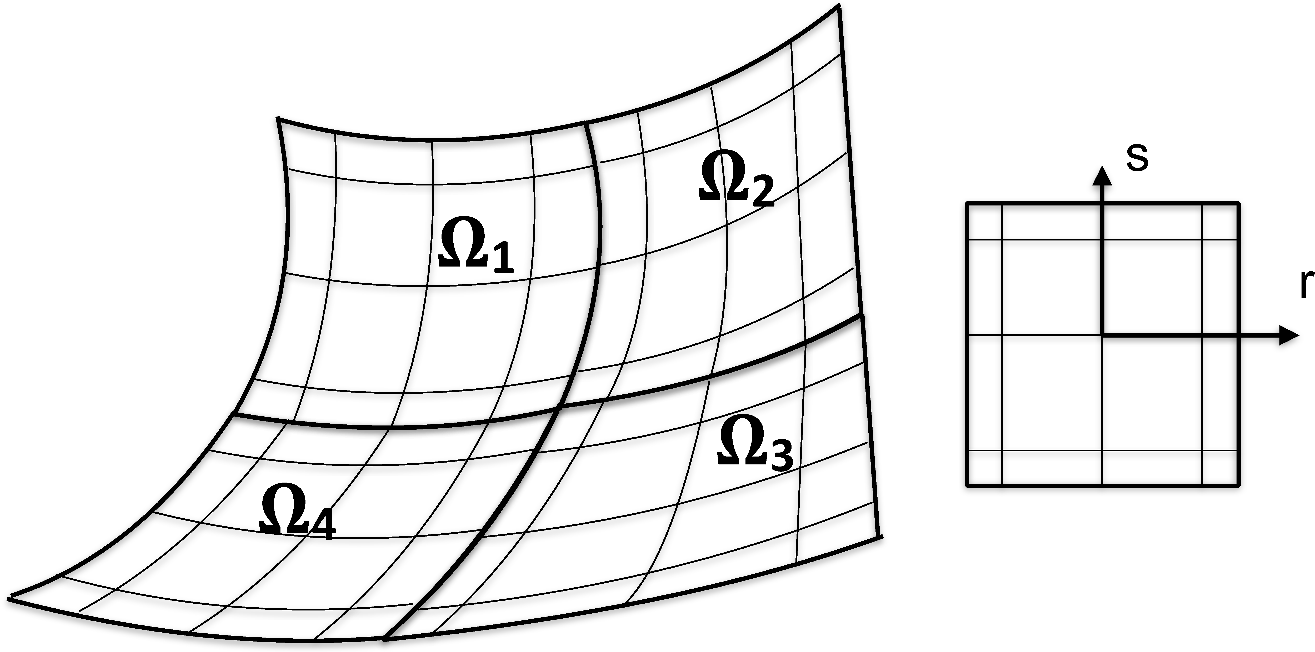
\includegraphics[width=8.0cm]{elements}
\caption{A schematic representation of spectral elements and the reference element in two dimensions.}
\label{elements}
\end{figure}

Figure~\ref{elements} also illustrates how a point $\bx\in\Omega_e$ is isoparametrically mapped to
$\mathbf{r}\equiv\left(r,s,t\right)^{\Txp}=\left(r_1,r_2,r_3\right)^{\Txp}$ in the reference element
$\Oh=[-1,1]^3$,
This transformation has, $\forall \mathbf{x}\in\Omega_e$,
Jacobian $J(\mathbf{x})\equiv|\partial \mathbf{x}/\partial \mathbf{r}|$ and
metrics $\partial r_i/\partial x_j$.

We integrate the right-hand-side (RHS) of Equation~\ref{dghweak} by parts a second time to get
the \textbf{``strong'' form} of the weighted residual statement,
\begin{equation}
\int_{\Omega_e} v(\bx) \pp{\bU(\bx)}{t}dV = 
\int_{\Omega_e} v \nabla \cdot \bH\, dV  
-\int_{\dO_e} v(\bx) \left(\bH-\bH^{\ast}\right) \cdot \bhn dA +
\int_{\Omega_e} \mathbf{R}(\bx) v(\bx) dV.
\label{dghstrong}
\end{equation}
The distinction between weak and strong forms is ultimately unimportant in DGSEM,
but strong form (Equation~\ref{dghstrong}) is clearer and more convenient.

\subsection{Quadrature and approximation}
All integrals in Equation~\ref{dghstrong} are now approximated by
\textbf{Gaussian quadrature}, as described in \S whatever of \cite{dfm02}.
We evaluate the solution $\bU$ and various functions of it (like fluxes $\bH$ and
source terms $\mathbf{R}$) on a grid of $N^3$ \textbf{Gaussian quadrature nodes}
within each element. This means:
\begin{enumerate}
\item The approximation space $\chi$ becomes $[\mathbb{P}^{N-1}]^3$, a Cartesian product of the space of all
polynomials of degree $N-1$.
\item The basis functions are a \textbf{nested tensor product} of the \textbf{interpolating Lagrange
polynomials} evaluated on $N^2$ lines of $N$ Gaussian quadrature nodes. This is
described in more detail in \S of \cite{dfm02}.
\item The discrete unknowns are the \textbf{nodal values} $\bU(x_i,y_j,z_k)$ at each of the $N^3$ Gaussian nodes in each element.
\end{enumerate}
Finally, within the family of Gaussian quadrature we specifically choose the
\textbf{Gauss-Legendre-Lobatto (GLL)} nodes. Formulas for $\omega$ and $\mathbf{r}$ may be found in Appendix of \cite{dfm02}.

Nodal values at grid points within a given element are arranged into
vectors lexicographically:
\begin{equation}
\mathbf{u}\equiv\left[\begin{array}{c} U(x_1,y_1,z_1) \\  U(x_2,y_1,z_1) \\ \vdots \\ U(x_N,y_N,z_N) \end{array}\right],
\mathbf{v}\equiv\left[\begin{array}{c} v(x_1,y_1,z_1) \\ v(x_2,y_1,z_1) \\  \vdots \\ v(x_N,y_N,z_N) \end{array}\right],
\mathbf{h}_1\equiv\left[\begin{array}{c} H_x(U(x_1,y_1,z_1))\\ H_x(U(x_2,y_1,z_1))\\   \vdots \\ H_x(U(x_N,y_N,z_N)) \end{array}\right],
\label{gridvects}
\end{equation}
with $u_l=U(x_i,y_j,z_k)$ when $l=i+N(j\!-\!1)+N^2(k\!-\!1)$.

These vectors may be catenated one element after the other into a vector $\buu_L$ of $N^3 K$ nodal
values for
the quadrature nodes in the entire mesh.

To assist notation for scalar multiplication, we introduce the diagonal matrix formed
from an arbitrary nodal vector $\mathbf{f}$
\begin{equation}
\mbox{diag}(\mathbf{f})\equiv \left[\begin{array}{cccc} f(x_1,y_1,z_1) & & & 0 \\
                                                        & \diagdown & & \\ 
                                                        & & f(x_i,y_j,z_k)  & \\
                                                        & & \diagdown & \\
                                                        & & & \\
                                                        0 & & & f(x_N,y_N,z_N)\end{array}\right].
\label{diagalot}
\end{equation}

Consider the left-hand-side of Equation~\ref{dghstrong}. Approximating everything with
the nodal representation on $N^3$ GLL points described above,
means our discrete equation becomes, at the top level,
\begin{equation}
\int_{\Omega_e} v(\bx) \pp{\bU(\bx)}{t}dV \approx \bv^{\Txp}\mathbf{B}\pp{\bu}{t} =
\mbox{RHS},
\label{firstdiscrete}
\end{equation}
where RHS is the right-hand-side of Equation~\ref{dghstrong}
evaluated at each GLL node. Bold-faced quantities are nodal vectors (Equation~\ref{gridvects}) including
the mass matrix $\mathbf{B}$,
\begin{equation}
\mathbf{B}\equiv \left[\begin{array}{ccc} \diagdown & & 0 \\ &  \omega_i\omega_j\omega_k J(\mathbf{x}(r_i,s_j,t_k)) &  \\  0 & & \diagdown \end{array}\right],
\label{masslex}
\end{equation}
where $\omega_i$ is the GLL quadrature weight associated with the $i$\nth quadrature
node,
and $J_e(\mathbf{x})$ is the Jacobian $J$ of the mesh transformation described
above at the GLL points within $\Omega_e$.

The Galerkin statement is enforced for all possible test functions in $\chi$ by
equating coefficients of the test function $\mathbf{v}$ on both sides of Equation~\ref{firstdiscrete}.
%\textbf{It suffices for me to state that
%any operation in the volume integral in Equation~\ref{dghstrong} using the transpose
%of a matrix or a Kronecker product labeled as a transpose is really being applied to the test functions.}
Further multiplication of Equation~\ref{firstdiscrete} by $\mathbf{B}^{-1}$ produces the semidiscrete method of lines
\begin{equation}
\pp{\bu}{t} =\mathbf{B}^{-1}\mbox{RHS}=I_{\mbox{vol}}-I_{\mbox{sfc}},
\label{dgsemifinal}
\end{equation}
which may be integrated in time to solve for the nodal values $\bu$ of the conserved variables.
Right-hand-side terms in Equation~\ref{dgsemifinal} are essentially the effects
contributions of individual GLL nodes to integrals (hence the ``I''
abbreviation). We describe those in the following section.

\section{Split forms of evaluating summation-by-parts operators\label{splitform}}
% MAKE SURE
%\bh and \bH are not confused
%\bh_m is used where appropriate for a nodal vector of a single unknown's flux
% H_m
We're solving a differential equation. We need to take derivatives of things
like $U$ and $\mathbf{H}$ approximated by polynomials on each element.
Finite differences are appropriate for computing derivatives of interpolating polynomials.
Algorithms are commonplace for finite differences on each of $N$ points expressed as
products between a $N\times N$ differentiation matrix $\mathcal{D}$ and a
vector of $N$ nodal values in one spatial dimension,
\begin{equation}
\mathcal{D}\bv \approx\left[\left.\dd{v}{r}\right|_{r_1},\, \cdots,\,\left.\dd{v}{r}\right|_{r_N} \right]^{\Txp}.
\label{diffmat1D}
\end{equation}
$\mathcal{D}$ is computed in Nek5000 using formulas derived in \cite[\S]{dfm02}.

Derivatives of $U$ for all $N^3$ GLL nodes in $\Omega_e$ in each of the three coordinate directions on
$\Oh$ are evaluated via the triple Kronecker product (see \cite[\S]{dfm02}) of $\mathcal{D}$ with
$\mathbf{I} \in\mathbb{R}^{N\times N}$:
\begin{equation}
\mathbf{D}_r=\mathbf{D}_{r_1}=\mathbf{I}  \otimes \mathbf{I} \otimes \mathcal{D}, \quad
\mathbf{D}_s=\mathbf{D}_{r_2}=\mathbf{I}  \otimes \mathcal{D}\otimes \mathbf{I} , \quad
\mathbf{D}_t=\mathbf{D}_{r_3}=\mathcal{D} \otimes \mathbf{I} \otimes \mathbf{I}.
\label{diffkron}
\end{equation}

On the GLL nodes, $\mathcal{D}$ has the \textbf{summation-by-parts property}:
\begin{equation}
\left(\mathbf{B}\mathcal{D}\right)^{Txp}+\mathbf{B}\mathcal{D}=\mbox{diag}\left(\left[-1,0,\dots,0,1\right]\right),
\label{SBP}
\end{equation}
which means that integration by parts in inner products like Equations~\ref{dghweak} and~\ref{dghstrong}
is done \emph{exactly} at the discrete level \emph{even if} 
the underlying quadrature is not itself exact.
Na{\"i}vely, we would write $I_{\mbox{vol}}$ in Equation~\ref{dgsemifinal} by
approximating the volume integral\footnote{The Einstein summation convention
applies to multiplication of derivatives in the direction $i$ on the GLL grid with flux in the
physical direction $j$.}
\begin{equation}
\sum_{e=1}^{nelt}\int_{\Omega_e} v \nabla \cdot \bH\, dV \approx
\bv^{\Txp}\mathbf{B}\mathbf{D}_i\left[\mbox{diag}\left(\frac{\partial r_i}{\partial x_j}\right)\bh_j\right],
\label{badvolint}
\end{equation}
where $\bh_j$ is the flux in the $x_j$ direction at the GLL nodes on all elements. We would then equate coefficients of $\bv$ and left multiply by
$\mathbf{B}^{-1}$ to get $I_{\mbox{vol}}$. However, it turns out\cite{CarpenterESSC} Equation~\ref{badvolint}
is itself further approximated by \textbf{a subcell flux difference}. Considering
a single GLL grid line on an undeformed element (such that $r=x_1$ for brevity, Fisher\cite{FisherJCP252}
proved\footnote{Cartesian indices in parentheses like ``$(i)$'' refer to the
$i^{\mbox{th}}$ element of an array and are \emph{not} subject to summation
convention.}
\begin{equation}
\left(\mathbf{D}_r\mathbf{h}_r\right)_{(ijk)}\approx
\frac{F_{(i+1,jk)}-F_{(ijk)}}{\omega_i}
\label{travis}
\end{equation}
to within the truncation error of the Lagrange polynomials on GLL nodes
with nodal values of fluxes $\bh$. Fisher introduced a \textbf{auxiliary flux function} $F$
that provided a way of enforcing bounds on fluxes \emph{even in the face of
quadrature errors in evaluating them.} The importance of this for stabilization
will be discussed in \S.

Finally, Fisher derived a \textbf{two-point split form} for Equation~\ref{travis}
that allowed (further) approximation of $F$ with \emph{yet another} flux function $F^{\#}$
\begin{equation}
\frac{F_{(i+1,jk)}-F_{(ijk)}}{\omega_i}\approx 2
\sum_{l=1}^N\mathcal{D}_{il}F^{\#}\left(\bu_{(ijk)},\bu_{(ljk)}\right),
\label{finally2pt}
\end{equation}
where $F^{\#}\left(\bU_a,\bU_b\right)$ is a flux function of two arguments instead of one!
At the very least, it must be consistent with the physical flux function.
%given conserved variable (numbered $m\in[1,5]$ below):
\begin{equation}
%F_m^{\#}\left(\bU,\bU\right)=H_m(\bU)
\bF^{\#}\left(\bU,\bU\right)=\bH(\bU)
\label{consistency}
\end{equation}
and symmetric in its two arguments.

So, to summarize, Equation~\ref{finally2pt} is, for system-dependent choices of
$\mathbf{F}^{\#}$ to be shown in \S, a \emph{stabilizing} way of approximately
evaluating the volume integral in Equation~\ref{dghstrong} for schemes based on
summation-by-parts (SBP) operators. Finite differences on GLL nodes in DGSEM are
SBP operators. While Equation~\ref{finally2pt} disrupts the matrix-vector
product $\mathbf{Du}$, it retains $N^4$ scaling in higher dimensions and promises
some unique stability properties on top of conservation and high-order accuracy\cite{walchidk}.
As a notational shorthand, we abbreviate Equation~\ref{finally2pt} as
\begin{equation}
\mathbb{D}(F^{\#})\equiv 2
\sum_{l=1}^N\mathcal{D}_{il}F^{\#}\left(\bu_{(ijk)},\bu_{(ljk)}\right),
\label{theotherd}
\end{equation}
where $F^{\#}\left(\bU_a,\bU_b\right)$ is a flux function of two arguments instead of one!
At the very least, it must be consistent with the physical flux function for a

Gassner, Winters and Kopriva\cite{splitformnodaldg} (and the works cited therein)
derive and explore several properties and features of these
``\textbf{two-point split forms}'' for the Euler equations. They transform them
to deformed spectral elements as follows.
Let indices \emph{i,j,k,l} denote individual GLL nodes within $\buu$ in three-dimensional storage or matrix elements.
First, fluxes must be transformed in a freestream-preserving way into the
\textbf{contravariant frame} aligned along the GLL grid within a given element.
Again, we subscript $\bH=\left(\bH_1,\bH_2,\bH_3\right)$ by the physical-space
direction $j\in[1,3]$. Again, we distinguish Cartesian tensor indices from GLL
nodes and matrix elements by writing, for example, the $x_2$-direction flux at
the $i^{\mbox{th}}$ GLL node as $H_2\left(\bU_{(i)}\right)$ and \emph{demanding
that summation convention apply} to the index on $H$ but \emph{NOT} to the
index on $\bU$!!!
Then, for a given conserved variable, the integrand in the volume integral in Equation~\ref{dghstrong} becomes
% DONT CRY. PiCK YOURSELF UP OFF HTE FLOOR. NOW
% ANSWER ONE QUESTION
% IS rx MULTIPLIED BY J IN THE 2-POINT CODE OR NOT?
\begin{equation}
\left[\mathbf{D}_r\mathbf{h}\right]_{(ijk)}\approx
\left[\mathbb{D}_r\left(F^{\#}\right)\right]_{(ijk)}\equiv
2\sum_{l=1}^N\mathcal{D}_{(il)}
\left\{\left\{J\mbox{diag}\left(\frac{\partial r_1}{\partial x_k}\right)\right\}\right\}_{((i,l)jk)}F^{\#}_k\left(\bU_{(ijk)},\bU_{(ljk)}\right),
\label{splitr}
\end{equation}
\begin{equation}
\left[\mathbf{D}_s\mathbf{h}\right]_{(ijk)}\approx
\left[\mathbb{D}_s\left(F^{\#}\right)\right]_{(ijk)}\equiv
2\sum_{l=1}^N\mathcal{D}_{(jl)}
\left\{\left\{J\mbox{diag}\left(\frac{\partial r_2}{\partial x_k}\right)\right\}\right\}_{(i(j,l)k)}F^{\#}_k\left(\bU_{(ijk)},\bU_{(ilk)}\right),
\label{splits}
\end{equation}
\begin{equation}
\left[\mathbf{D}_t\mathbf{h}\right]_{(ijk)}\approx
\left[\mathbb{D}_t\left(F^{\#}\right)\right]_{(ijk)}\equiv
2\sum_{l=1}^N\mathcal{D}_{(kl)}
\left\{\left\{J\mbox{diag}\left(\frac{\partial r_3}{\partial x_k}\right)\right\}\right\}_{(ij(k,l))}F^{\#}_k\left(\bU_{(ijk)},\bU_{(ijl)}\right),
\label{splitt}
\end{equation}
% DONT CRY. PiCK YOURSELF UP OFF HTE FLOOR. NOW
% ANSWER ONE QUESTION
% IS rx MULTIPLIED BY J IN THE 2-POINT CODE OR NOT?
where we have introduced notation for an \textbf{average} between two grid points
along a line of fixed $r$ in the grid on the reference element,
\begin{equation}
\left\{\left\{U\right\}\right\}_{((i,l)jk)}\equiv\frac{1}{2}\left(U_{(ijk)}+U_{(ljk)}\right),
\label{avgr}
\end{equation}
\begin{equation}
\left\{\left\{U\right\}\right\}_{(i(j,l)k)}\equiv\frac{1}{2}\left(U_{(ijk)}+U_{(ilk)}\right),
\label{avgs}
\end{equation}
\begin{equation}
\left\{\left\{U\right\}\right\}_{(ij(k,l))}\equiv\frac{1}{2}\left(U_{(ijk)}+U_{(ijl)}\right).
\label{avgt}
\end{equation}
These averages will be needed to define various flux functions of interest too. Equations~\ref{splitr} through~\ref{splitt} are applied component-wise to each of the conserved variables in
$\mathbf{H}$ (with correponding components in $\mathbf{F}$).

So, we have an elaborate way of writing the discrete approximation to the
volume integral on the right-hand-side of Equation~\ref{dgsemifinal}:
\begin{equation}
I_{\mbox{vol}}\equiv \mbox{diag}\left(\frac{1}{J}\right)\sum_{j=1}^3\mathbb{D}_j\bh
\label{shortvol}
\end{equation}
where $\mathbb{D}_j$ is defined by Equations~\ref{splitr} through~\ref{splitt}.

\subsection{A short note on strong form}
The extra discontinuous surface flux in Equation~\ref{dghstrong} is evaluated
on the fly by modifying the differentiation matrix $\mathcal{D}$. In the
code,
\begin{equation}
dstrong=\mathcal{D}-2\mbox{diag}\left(\left[-1/\omega_1,0,\dots,0,1/\omega_N\right]\right)\mathbb{D}
\label{dstrong}
\end{equation}
is enough to include the surface integral from integrating by parts twice. dstrong
is evaluated in chainrule\_metrics subroutine of intpdiff.
%LINK THAT

%The general flux function for all 5 governing equations is now noted 

\section{Surface integral terms}%\label{sfcmath}}\index{Surface\_math@{Surface\_math}}
%INDEX YOUR SHIT!!!
\begin{equation}
I_{\mbox{sfc}}=-\left(\sum_{f=1}^6
\mathbf{E}^{(f)\Txp}\mathbf{B}^{(f)}\left[\mbox{diag}\left(\bhn^{(f)}_j\right)\left(\bh_j-\bh^{\ast(f)}_j\right)\right]\right).
\label{isfc} % was dgweak
\end{equation}
where the ``face'' mass matrix $\mathbf{B}^{(f)}$ is
\begin{equation}
\mathbf{B}^{(f)}\equiv \left[\begin{array}{ccc} \diagdown & & 0 \\ &  \omega_i\omega_j J^{(f)}(\mathbf{x}(r_i,s_j)) &  \\  0 & & \diagdown \end{array}\right]\in\mathbb{R}^{N^2 \times N^2},
\label{massA}
\end{equation}
and we note that the vectors of nodal values $\bhn^{(f)}_j$ and $\bh^{(f)}_j$ in
\ref{isfc} have only $N^2$ elements since they correspond to GLL nodes on face $f$.
Crucially, we have also introduced the \emph{restriction operator} $\mathbf{E}^{(f)}\in\mathbb{R}^{N^2\times N^3}$ for the $f^{\mbox{th}}$ face in \ref{isfc}.
The restriction operator is defined as an indicator that is zero for all GLL nodes except those on the
element faces $\dO_e$, an operation easily expressed as Kronecker products (for example, in the
$r_1-$direction for $f=1$ at $r=r_1=-1$)
\begin{equation}
\bE^{(1)}=\bI\otimes \bI\otimes \mathcal{E}_1
\label{bigE1}
\end{equation}
of the $\bI\in\mathbb{R}^{N\times N}$ identity matrix with unit vectors $\mathcal{E}\in\mathbb{R}^N$
(in \ref{bigE1}, $\mathcal{E}_1\equiv\left(1,0,\dots, 0\right)^{\Txp}$).
Similar indicators may be built up in the $r_2$- and $r_3$-directions by following the ordering of
Kronecker products in \ref{diffkron}.
%Substituting \ref{isfc} into~\ref{sfcintcube} and applying the matrix identity $(\bA\bB)^{\Txp}=\bB^{\Txp}\bA^{\Txp}$ discretely represents the surface integral of the numerical flux on $\Oh$:
Applying the matrix identity $(\bA\bB)^{\Txp}=\bB^{\Txp}\bA^{\Txp}$ to Equation~\ref{isfc} discretely represents the surface integral of the numerical flux on $\Oh$:
\begin{equation}
\sum_{f=1}^6\iint\displaylimits_{-1}^1 v(\br) H^{\ast(f)}_j\hat{n}^{(f)}_j J^{(f)}\, dr \, ds=\sum_{f=1}^6
\bv^{\Txp}\mathbf{E}^{(f)\Txp}\mathbf{B}^{(f)}\left(\left[\mbox{diag}\left(\bhn^{(f)}_j\right)\bh^{\ast(f)}_j\right]\right).
\label{sfcintmatvect}
\end{equation}

\subsection{Surface flux functions}%\label{sfcmath}}\index{Surface\_math@{Surface\_math}}
%INDEX YOUR SHIT!!!
According to a vast body of literature not cited here, summation-by-parts (SBP)
operators need appropriate boundary treatment to behave well. These are
called \textbf{simultaneous approximation terms} (SAT), and the family of
methods that have nice conservation and stability properties always have these
two things together and are called ``SBP-SAT'' methods. For the purposes of
DGSEM, Gassner, Winters \& Kopriva \cite[Eq]{} recommend a numerical flux
function consisting of a symmetric function and an extra dissipative term:
\begin{equation}
\bH^{\ast}\left(\bU^-,\bU^+\right)=\mathbf{F}^{\#}\left(\bU^-,\bU^+\right)+\mathbf{F}_{\mbox{stab}}\left(\bU^-,\bU^+\right),
\label{numfluxfinally}
\end{equation}
where $\bH^{\ast}$ is the flux between neighboring elements
in Equation~\ref{dghstrong}. Gassner, Winters and Kopriva have indeed recycled
the same split-form flux function used in Equations~\ref{splitr} through~\ref{splitt},
but instead of evaluating it at two separate points, they evaluate it using the
two values present at each interface between elements.

SAT tend to be dissipative, and the dissipative nature of $\bH^{\ast}$ in
DG is needed in DGSEM as well. $\bF^{\#}$ is augmented with a stabilizing
flux $\bF_{\mbox{stab}}$. Examples of this will be given in \S.


\chapter{Time-marching and top-level assembly}
A parallel program like CMT-nek only fits
\textbf{nelt} elements on the memory available to a single MPI task. \textbf{lelt}
is the maximum number of elements that may be stored on a single MPI task. It is
set in the SIZE file. Quantities such as Equation~\ref{gridvects} and~\ref{diagalot}
are stored in multidimensional arrays to facilitate nested-tensor-product operations.
An example is the storage of the values of the $x$-coordinate at grid points in each element in
the mesh that lies on a given MPI task.
\begin{table}
\begin{tabular}{|c|c|c|c|}
\hline
Mathematical variable & variable in code & common & include file \\
$N$ & lx1=ly1 &  & SIZE \\
dimension $d$ & ldim &  & SIZE \\
\hline
grid coordinate of GLL nodes & variable in code & common & include file (core/)\\
\hline
$x$ & xm1(lx1,ly1,lz1,lelt) & /gxyz/ & GEOM \\
$y$ & ym1(lx1,ly1,lz1,lelt) & /gxyz/ & GEOM \\
$z$ & zm1(lx1,ly1,lz1,lelt) & /gxyz/ & GEOM \\
\hline
\end{tabular}
\caption{Declarations and locations for basic geometry}
\label{tab:xm1gridvect}
\end{table}

\textbf{Note on lz1}: The triple ``lx1,ly1,lz1'' is mandated for all declarations and loops intended
to cover or otherwise refer to the grid of $N^d$ quadrature nodes within an element. 
Although lx1, ly1 and lz1 are not
arbitrary, the limited rules surrounding their use does make it easier to reuse code
and share it between 2D and 3D cases. An important rule for such sharing is in
Table~\ref{tab:dimz}.
\begin{table}
\begin{tabular}{|c|c|c|}
\hline
case & value of ldim & value of lz1 \\
\hline
two-dimensional, $d=2$ & ldim=2 & lz1=1 \\
three-dimensional, $d=3$ & ldim=3 & lz1=lx1=ly1$=N$ \\
\hline
\end{tabular}
\caption{Problem dimensionality and how the SIZE file can take care of so many things}
\label{tab:dimz}
\end{table}

Table~\ref{tab:mass} shows where quadrature-related
quantities live (again, in core/, not core/cmt/)

\begin{table}
\begin{tabular}{|c|c|c|c|}
\hline
Mathematical variable & variable in code        & common & include file \\
\hline
$\mathbf{B}$          & bm1(lx1,ly1,lz1,lelt)   & /mass/ & MASS \\
$J$                   & jacm1(lx1,ly1,lz1,lelt) &  /giso1/ & GEOM \\
$r$, $s$ and $t$      & zgm1(lx1,3)             &  /gauss/ & WZ \\
$\omega_i$, $i=1,\dots,N$ & wxm1(lx1)           &  /gauss/ & WZ \\
\hline
\end{tabular}
\caption{Declarations and locations for quadrature}
\label{tab:mass}
\end{table}

\section{Data structure of surface quantities}\label{sfcdata}\index{Surface\_data@{Surface\_data}}
Surface terms and nodal vectors of surface quantities are stored in a different format from
the one introduced in Table~\ref{tab:soln} for general storage of variables on the whole mesh.
Every face point in every element, from an element-centered point of view (i.e., 
every element has is own copy of values at nodes lying on its 2*ldim faces), fits
in an array of size
\begin{verbatim}
nfq=lx1*lz1*2*ldim*nelt
\end{verbatim}%\label{nfq}
ordered according to:
\begin{verbatim}
dimension(lx1,lz1,2*ldim,lelt)
\end{verbatim}%\label{pileoffaces}
I call this a ``pile of faces.''
I also made a common block to store many of them, /CMTSURFLX/, that I had intended to be somewhat malleable.
Thus, quantities in it are very large 1D arrays, indexed by whole-number multiples of nfq, and
passed to different subroutines. \textbf{ONLY inside subroutines} are \textbf{dummy arguments} dimensioned
(lx1,lz1,2*ldim,lelt). 
Every face has lx1$\times$lz1 nodes on the face. This makes it suitable for both 2D (lz1=1) and 3D (lz1=lx1=ly1=$N$) meshes.
Every element has 2*ldim faces, and arrays in /CMTSURFLX/ (and in core commons like /GSURF/ and /FACEWZ/)
store nodal vectors on faces contiguously element by element.

Subroutines that index face nodes within arrays dimensioned (lx1,ly1,lz1,lelt) storing full fields
and copy such data into arrays dimensioned (lx1,lz1,2*ldim,lelt) are stored in face.f
(\S~\ref{face_8f}).

Each GLL node in each element making up
$\buu_L$, the union of $\bu$ for all $K$ elements, is integrated in time in this subroutine
via explicit time marching to discretizes the
the left-hand-side time derivative of Equation~\ref{dgsemifinal}.
We choose the third-order total-variation-diminishing\footnote{Equivalent to
the strong-stability-preserving explicit RK scheme at this order} Runge-Kutta scheme (TVDRK3) in low-storage form.
We advance from $t_n$ to $t_{n+1}=t_n+\Delta t$ via
\begin{align}
\buu_L^{(1)}&=\buu_L^{(n)}+\Delta t \mbox{RHS}(\buu_L^{(n)}), \nonumber \\
\buu_L^{(2)}&=\frac{3}{4}\buu_L^{(n)}+\frac{1}{4}\buu_L^{(1)}+\frac{1}{4}\Delta t\, \mbox{RHS}(\buu_L^{(1)}), \label{eq:rk3} \\
\buu_L^{(n+1)}&=\frac{1}{3}\buu_L^{(n)}+\frac{2}{3}\buu_L^{(2)}+\frac{2}{3}\Delta t\, \mbox{RHS}(\buu_L^{(2)}). \nonumber
\end{align}


\chapter{Governing equations and fluid properties}
We now divide the flux function $\mathbf{H}$ into
\begin{equation}
\bH=\bH_c(\bU)+\bH_d(\bU,\nabla \bU),
\label{convanddiff}
\end{equation}
where $\bH_c$ is the \textbf{convective flux} function and $\bH_d$ is the \textbf{diffusive flux} function.
The convective fluxes come from the Euler equations of gas dynamics and the diffusive
fluxes come from artificial viscosity used to capture shocks on spectral elements.
\section{Euler equations of gas dynamics\label{sec:gaseom}}
We now present the Euler equations of gas dynamics
In this section, bold-faced quantities are vectors in $\mathbb{R}^3$ except for the conserved variables
$\bU$,
\begin{equation}
  \mathbf{U}=\left[\begin{array}{l} \phi_g \rho \\ \phi_g \rho u \\ \phi_g \rho v \\ \phi_g \rho w \\ \phi_g \rho E \end{array}\right],
  \label{uvect}
\end{equation}
which live in $\mathbb{R}^5$. Conserved variables and their inviscid fluxes\footnote{\textcolor{red}{but not their viscous fluxes}}
are weighted by the \textbf{gas volume fraction} $\phi_g$. To more easily subscript flux vectors we write the $m$\nth component of $\bU$ as being governed by the
conservation law
\begin{equation}
%\pp{U_m}{t} + \divnce \bH_m=0,\, m=1,\dots,5.%R_m, I don't like having a period after an integer
\pp{U_m}{t} + \divnce \bH_m=R_m,\, m\in\left[1,5\right].%R_m,
\label{conslaw}
\end{equation}
The gas velocity $\mathbf{v}$ is % and spatial coordinate $\mathbf{x}$ are
\begin{equation}
\mathbf{v}=\left[\begin{array}{l} u \\ v \\ w \end{array}\right]=
\left[\begin{array}{l} v_1 \\ v_2 \\ v_3 \end{array}\right],%, \qvad
%\mathbf{x}=\left[\begin{array}{l} x \\ y \\ z \end{array}\right]=
%\left[\begin{array}{l} x_1 \\ x_2 \\ x_3 \end{array}\right],
\label{uxpedantic}
\end{equation}
and $\rho$ is the gas density, $E$ is the mass-specific total energy $e+\frac{1}{2}|\mathbf{v}|^2$ of
the gas, $e$ is the gas internal energy, and $p$ is the thermodynamic gas pressure.

$\bH_m(\bU,\nabla \bU) \mathbb{R}^{5\times 3}\rightarrow \mathbb{R}^3$
is the flux vector of equation~$m$. Like \ref{convanddiff},
$\bH_m$ is made up of a convective flux $\bH_{m,c}(\bU)$ and a
diffusive flux $\bH_{m,d}(\bU,\nabla \bU)$. We consider the convective
fluxes first. For gas density $\bH_{1,c}(\bU)$ is
\begin{equation}\label{convh1}
   \bH_{1,c}=\phi_g\rho \mathbf{v}= \left[U_2,U_3,U_4\right]^{\Txp}.
\end{equation}
For gas momentum $U_{2-4}$, the convective fluxes are
\begin{align}
   \bH_{2,c}=\phi_g\left[\begin{array}{l} \left(\rho u\right)u \!+\! p \\
                                               \left(\rho u\right)v \\
                                               \left(\rho u\right)w \end{array}\right],
   \bH_{3,c}=\phi_g\left[\begin{array}{l} \left(\rho v\right)u \\
                                               \left(\rho v\right)v \!+\! p \\
                                               \left(\rho v\right)w \end{array}\right], %\nonumber \\
   \bH_{4,c}=\phi_g\left[\begin{array}{l} \left(\rho w\right)u \\
                                               \left(\rho w\right)v \\
                                               \left(\rho w\right)w \!+\! p \end{array}\right],  \label{convh2to4}
\end{align}
and, for total energy $\rho E$,
\begin{equation} \label{convh5}
   \bH_{5,c}= \phi_g \mathbf{v}\left(\rho E +p\right).
\end{equation}

The system is closed by an equation of state,
\begin{equation}
\left[p,T\right]=\mbox{EOS}\left(\rho,e\right).
\label{eos}
\end{equation}
Internal energy per
unit mass $e=E-\frac{1}{2}|\mathbf{v}|^2$ is related to gas temperature $T$ by the intensive property $c_v$, the constant-volume specific heat, such that
\begin{equation}
   e=\int c_v(T)dT.
   \label{cvt}
\end{equation}
Generally, \ref{cvt} must be solved for temperature $T$ implicitly, iteratively,
or via tabulation.
For calorically perfect gases, $c_v$ is constant. For both thermally and
calorically perfect gases, pressure is obtained last via
\begin{equation}
p=\rho R T,
\label{eos_tpg}
\end{equation}
where the specific gas constant $R=\left(\gamma-1\right)c_v$ requires the specification
of $\gamma=c_p/c_v$, the ratio of constant-pressure specific heat $c_p$ to $c_v$. Finally, the sound
speed is
\begin{equation}
a=\sqrt{\frac{\gamma p}{\rho}}.%=\sqrt{\gamma RT}.
\label{asndtpg}
\end{equation}


Vectors of nodal values are usually stored consecutively in
multidimensional arrays whose ``outermost'' index is fixed for that particular quantity.
\textcolor{red}{As an exception, conserved variables are dimensioned element-outermost, and the second-to-last dimension
is fixed for a given conserved variable.} The indexing for this purpose is given in Table~\ref{tab:cvar}.

\begin{table}
\begin{tabular}{|c|c|}
\hline
conserved variable in \S\ref{sec:gaseom} & index in U(ix,iy,iz,:,e) \\
\hline
mass $\phi_g \rho$ & irg=1 \\
$x$-momentum $\phi_g \rho u$ & irpu=2 \\
$y$-momentum $\phi_g \rho v$ & irpv=3 \\
$z$-momentum $\phi_g \rho w$ & irpw=4 \\
total energy per unit mass, gas $\phi_g \rho E$  & irpe=5 \\
\hline
\end{tabular}
\caption{Declarations and locations for conserved variables (Equation~\ref{uvect}) in CMT-nek in U in /solnconsvar/ in CMTDATA. Indices are parameters at the end of CMTDATA.}
\label{tab:cvar}
\end{table}

Table~\ref{tab:soln} lays out where some of the physical variables are declared and stored. We recycle
many of nek5000's arrays, \textcolor{red}{with some abuse.} In the classic $P_NP_{N-2}$ spectral
element method, pressure is stored at nodal values on a separate mesh (m2=``mesh 2'') of Gauss-Legendre(GL) and not GLL quadrature nodes. \textcolor{red}{CMT-nek may need this mesh to follow Fisher \& Carpenter in a DGSEM formulation with the summation-by-parts property. For now,  however, pressure is not staggered.}
\textcolor{red}{CMT-nek must be run in the $P_N P_N$ mode with lx2=lx1, and using mesh-1 metrics for
everything, including pr, which is not correct for nek5000 in general.}
\begin{table}
\begin{tabular}{|c|c|c|c|c|}
\hline
primitive variable in \S\ref{sec:gaseom} & variable in code & outer index & common & include file \\
\hline
$x$-velocity $u$, Eq.~\ref{uxpedantic} & vx(lx1,ly1,lz1,lelt) & & /vptsol/ & core/SOLN \\
$y$-velocity $v$, Eq.~\ref{uxpedantic} & vy(lx1,ly1,lz1,lelt) & & /vptsol/ & core/SOLN \\
$z$-velocity $w$, Eq.~\ref{uxpedantic} & vz(lx1,ly1,lz1,lelt) & & /vptsol/ & core/SOLN \\
thermodynamic gas pressure $p$ & pr(lx2,ly2,lz2,lelv) & & /cbm2/ & core/SOLN \\
gas temperature $T$ & t (lx1,ly1,lz1,lelt,ldimt) & 1 & /vptsol/ & core/SOLN \\
gas density $\rho$ & vtrans(lx1,ly1,lz1,lelt,ldimt1) & irho & /vptsol/ & core/SOLN \\
mass-weighted specific heat $\rho c_p$ & vtrans(lx1,ly1,lz1,lelt,ldimt1) & icp & /vptsol/ & core/SOLN \\
mass-weighted specific heat $\rho c_v$ & vtrans(lx1,ly1,lz1,lelt,ldimt1) & icv & /vptsol/ & core/SOLN \\
isentropic sound speed $a$, Eq.~\ref{asndtpg}  & csound(lx1,ly1,lz1,lelt) & & /cmtgasprop/ & CMTDATA \\
\hline
\end{tabular}
\caption{Declarations and locations for CMT-nek primitive variables. Outer indices are parameters in CMTDATA}
\label{tab:soln}
\end{table}

Fluxes in the Euler equations (Equation~\ref{convh1} through~\ref{convh5}) are functions of
\textbf{primitive variables} (Table~\ref{tab:soln}) in addition to the primary unknowns, the conserved variables.
(Equation~\ref{uvect}).

\chapter{Right-hand-side evaluation: volume terms}
\section{Two-point flux functions}
Gaussian quadrature on $N$ GLL points exactly integrates a polynomial of order
${2(\!N\!-\!1\!)-1}$. However, nonlinear flux functions like
\ref{convh2to4} produce integrands that are rational functions of $\mathbf{U}$
since we are dividing by density to get velocity from momentum. Gaussian
quadrature at any order is not exact for rational integrands. %PROVE
Worse arithmetic than mere division is required by most state equations. 
integrated on only $N$ points. These errors tend to accumulate with time,
and something must be done to stabilize the scheme against their deleterious
effects.

The major motivation for \S\ref{splitform} is a robust stabilization scheme
for doing quadrature on these fluxes. Equation~\ref{finally2pt} has been
proven to guarantee that if the two-point form $\bF^{\#}$ conserves kinetic energy,
then a high-order SBP operator using it in Equations~\ref{splitr}
through~\ref{splitt} will do so exactly and discretely. %99% sure travis said this p.530
% of JCP 252
More importantly, if $\bF^{\#}$ is \textbf{entropy-stable} (provably increases
physical entropy or conserves it), then high-order SBP operators using it in
DGSEM will be discretely entropy-stable as well. A growing body of tests
\cite{WALCHCOMPARISONTODEAL} has shown that these discrete stability properties
are recovered without loss of formal order of accuracy in constructed solutions
and turbulent flows. Furthermore, these properties translate to better stability
at lower cost than in traditional
``overintegration\cite{KirbyKard}'' or ``dealiasing'' techniques.

We finally give some examples of the two-point flux functions that DGSEM depends on.
As usual, details and motivation may be found in Gassner, Winters and Kopriva\cite{}.
\subsection{Kennedy and Gruber}
The flux in Equation~(3.10) of Gassner, Winters \& Kopriva\cite{} is 
the kinetic-energy-preserving skew-symmetric split form of Kennedy \& Gruber\cite{kg}
reformulated for SBP operators in the form of Equation~\ref{finally2pt}. In
each coordinate direction this flux is, for all 5 conserved variables,
\begin{equation}
\bF_1^{\#}\left(\bu_{(ijk)},\bu_{(ljk)}\right),
\bF_2^{\#}\left(\bu_{(ijk)},\bu_{(ilk)}\right),
\bF_3^{\#}\left(\bu_{(ijk)},\bu_{(ijl)}\right),
\label{someargs}
\end{equation}
\begin{equation}
\bF_1^{\#}=\left[\begin{array}{c} \hat{\rho}\hat{u} \\
                               \hat{\rho}\hat{u}^2 + \hat{p} \\ 
                               \hat{\rho}\hat{u}\hat{v} \\ 
                               \hat{\rho}\hat{u}\hat{w} \\ 
                               \hat{u}\left(\hat{\rho}\hat{e} +\hat{p}\right)
              \end{array}\right], 
\bF_2^{\#}=\left[\begin{array}{c} \hat{\rho}\hat{v} \\
                               \hat{\rho}\hat{v}\hat{u} \\ 
                               \hat{\rho}\hat{v}^2 + \hat{p} \\ 
                               \hat{\rho}\hat{v}\hat{w} \\ 
                               \hat{v}\left(\hat{\rho}\hat{e} +\hat{p}\right)
              \end{array}\right], 
\bF_3^{\#}=\left[\begin{array}{c} \hat{\rho}\hat{w} \\
                               \hat{\rho}\hat{w}\hat{u} \\ 
                               \hat{\rho}\hat{w}\hat{v} \\ 
                               \hat{\rho}\hat{w}^2 + \hat{p} \\ 
                               \hat{w}\left(\hat{\rho}\hat{e} +\hat{p}\right)
              \end{array}\right], 
\label{kennedygruber}
\end{equation}
where the ``hat'' variables are actually function of the indicated quantity
at the two points upon which $\bF^{\#}_k$ acts. For the Kennedy-Gruber and other
energy-stable fluxes,
\begin{equation}
\hat{f}\left(\mathbf{f}_{(ijk)},\mathbf{f}_{(ljk)}\right)\equiv \left\{\left\{
f\right\}\right\}_{((i,l)jk)},
\label{ezhat}
\end{equation}
where Equation~\ref{avgr} defines the ``$\{\{\}\}$'' averaging operator.
Similar definitions exist for the grid lines in other directions on the reference
element. Thus, the Kennedy and Gruber flux is a \textbf{product of averages}
of quantities at the two points used to evaluate $\bF^{\#}$ in Equation~\ref{finally2pt}.


%\input{viscreg}
The volume integral term for the diffusive fluxes $\mbox{K}_{m,d}$ is, for the $m$\nth conserved variable,
\begin{equation}
\mbox{K}_{m,d}\equiv \mathbf{B}^{-1}\left(\mathbf{D}_{r_l}^{\Txp}
\left[\mbox{diag}\left(\pp{r_l}{x_i}\right)\mathbf{B}\left(\mathscr{A}_{mijL}
\left[\mbox{diag}\left(\pp{r_k}{x_j}\right)\mathbf{D}_{r_k} \mathbf{u}_L\right]\right)\right]\right),
\label{iku}
\end{equation}
where Einstein summation convention is used on all Roman subscripts. The ranges of these subscripts follow
their ordering in $\mathscr{A}_{mijL}$ (\ref{eq:vfjac,lazya}),  % must correctly couple all 5 governing equations
and $\bu_L$ refers to a nodal vector (\ref{gridvects}) of the $L$\nth conserved variable in
\ref{uvect}.

%--------------------------------
% INSERT FORMULATION THERE
%--------------------------------
\chapter{Module Index}
\section{Modules}
Here is a list of all modules\-:\begin{DoxyCompactList}
\item \contentsline{section}{Volume integral for inviscid fluxes}{\pageref{group__convhvol}}{}
\item \contentsline{section}{Surface integrals due to boundary conditions}{\pageref{group__bcond}}{}
\item \contentsline{section}{Volume integral for viscous fluxes}{\pageref{group__diffhvol}}{}
\item \contentsline{section}{Jacobians for viscous fluxes}{\pageref{group__vfjac}}{}
\item \contentsline{section}{Inviscid surface terms}{\pageref{group__isurf}}{}
\item \contentsline{section}{Viscous surface terms}{\pageref{group__vsurf}}{}
\item \contentsline{section}{Flux functions and wrappers}{\pageref{group__flux}}{}
\item \contentsline{section}{utility functions for manipulating face data}{\pageref{group__faceops}}{}
\item \contentsline{section}{structure for symmetric flux functions in split forms}{\pageref{group__twopoint}}{}
\item \contentsline{section}{flow field initialization routines}{\pageref{group__initialconds}}{}
\item \contentsline{section}{Thermodynamic state variables from conserved variables}{\pageref{group__state}}{}
\end{DoxyCompactList}

\chapter{File Index}
\section{File List}
Here is a list of all documented files with brief descriptions\-:\begin{DoxyCompactList}
\item\contentsline{section}{\hyperlink{bc_8f}{bc.\-f} \\*Boundary condition routines }{\pageref{bc_8f}}{}
\item\contentsline{section}{\hyperlink{diffusive__cmt_8f}{diffusive\-\_\-cmt.\-f} \\*Routines for diffusive fluxes. Some surface. Some volume. All pain. Jacobians and other factorizations }{\pageref{diffusive__cmt_8f}}{}
\item\contentsline{section}{\hyperlink{drive1__cmt_8f}{drive1\-\_\-cmt.\-f} \\*High-\/level driver for C\-M\-T-\/nek }{\pageref{drive1__cmt_8f}}{}
\item\contentsline{section}{\hyperlink{drive2__cmt_8f}{drive2\-\_\-cmt.\-f} \\*Mid-\/level initialization drivers. Not long for this world }{\pageref{drive2__cmt_8f}}{}
\item\contentsline{section}{\hyperlink{driver3__cmt_8f}{driver3\-\_\-cmt.\-f} \\*Routines for primitive variables, usr-\/file interfaces and properties. Also initializes flow field }{\pageref{driver3__cmt_8f}}{}
\item\contentsline{section}{\hyperlink{eqnsolver__cmt_8f}{eqnsolver\-\_\-cmt.\-f} \\*Routines for entire terms on R\-H\-S. Mostly volume integrals }{\pageref{eqnsolver__cmt_8f}}{}
\item\contentsline{section}{\hyperlink{face_8f}{face.\-f} \\*Low-\/level initialization drivers. Eventually to be superceded by nek5000 core D\-G handles and operators }{\pageref{face_8f}}{}
\item\contentsline{section}{\hyperlink{fluxfn_8f}{fluxfn.\-f} \\*Riemann solvers, other rocflu miscellany and two-\/point fluxes }{\pageref{fluxfn_8f}}{}
\item\contentsline{section}{\hyperlink{intpdiff_8f}{intpdiff.\-f} \\*Interpolation and differentiation routines not already provided by nek5000 }{\pageref{intpdiff_8f}}{}
\item\contentsline{section}{\hyperlink{outflow__bc_8f}{outflow\-\_\-bc.\-f} \\*Dirichlet states for outflow boundary conditions wrapper for other B\-C routines. Just one for now. More to come }{\pageref{outflow__bc_8f}}{}
\item\contentsline{section}{\hyperlink{step_8f}{step.\-f} \\*Time stepping and mesh spacing routines }{\pageref{step_8f}}{}
\item\contentsline{section}{\hyperlink{surface__fluxes_8f}{surface\-\_\-fluxes.\-f} \\*Routines for surface terms on R\-H\-S }{\pageref{surface__fluxes_8f}}{}
\item\contentsline{section}{\hyperlink{wall__bc_8f}{wall\-\_\-bc.\-f} \\*Dirichlet states for wall boundary conditions }{\pageref{wall__bc_8f}}{}
\end{DoxyCompactList}

\chapter{Module Documentation}
\hypertarget{group__convhvol}{\section{Volume integral for inviscid fluxes}
\label{group__convhvol}\index{Volume integral for inviscid fluxes@{Volume integral for inviscid fluxes}}
}
\subsection*{Functions/\-Subroutines}
\begin{DoxyCompactItemize}
\item 
subroutine \hyperlink{group__convhvol_ga77e7d7a46950fcbbf072e8e900cee272}{convective\-\_\-cmt} (e)
\begin{DoxyCompactList}\small\item\em Evaluates inviscid volume terms for all toteq equations in two-\/point split form (Equation~\ref{shortvol} and adds them to res1(\-:,\-:,\-:,e,\-:). \end{DoxyCompactList}\item 
subroutine \hyperlink{group__convhvol_ga72c1cbe51bc537e14ec8927e62f0e3f3}{fluxdiv\-\_\-2point\-\_\-noscr} (res, fcons, e, ja)
\begin{DoxyCompactList}\small\item\em Evaluates the two-\/point split form (Equations~\ref{splitr} through ~\ref{splitt}) of the volume integral $\int v \nabla\cdot\mathbf{H}^c dV$ and the discontinuous surface flux $\oint v \mathbf{H}^c\cdot\mathbf{n} dA$ for the inviscid flux function in a single element. \end{DoxyCompactList}\item 
subroutine \hyperlink{group__convhvol_gab4831bb28a78e1c8fd3ec09854bd15ad}{fluxdiv\-\_\-strong\-\_\-contra} (e)
\begin{DoxyCompactList}\small\item\em Computes $\int v \nabla\cdot\mathbf{H}^c dV$ in aliased strong form for element $e$, and increments res1 with it. \end{DoxyCompactList}\item 
subroutine \hyperlink{group__convhvol_gad9d70d83f1184d25495812d637698102}{evaluate\-\_\-aliased\-\_\-conv\-\_\-h} (e)
\begin{DoxyCompactList}\small\item\em Evaluates consistent (i.\-e. $F^{\#}(U_{i,j,k},U_{l,j,k})=H_{(eq),i},i=l$) flux function at all G\-L\-L nodes and stores it in convh. \end{DoxyCompactList}\item 
\hypertarget{group__convhvol_ga89ba8fe53f8afc523597773aca62a270}{subroutine \hyperlink{group__convhvol_ga89ba8fe53f8afc523597773aca62a270}{fluxdiv\-\_\-dealiased\-\_\-weak\-\_\-chain} (e)}\label{group__convhvol_ga89ba8fe53f8afc523597773aca62a270}

\begin{DoxyCompactList}\small\item\em $(\nabla v)\cdot \mathbf{H}^c=\mathcal{I}^{\intercal}\mathbf{D}^{\intercal}\cdots$ for equation eq, element e \end{DoxyCompactList}\item 
subroutine \hyperlink{group__convhvol_ga72103225babeca7679ef8b9a41d08f2e}{contravariant\-\_\-flux} (frst, fxyz, ja, nel)
\begin{DoxyCompactList}\small\item\em Transforms consistent (i.\-e. $F^{\#}(U_{i,j,k},U_{l,j,k})=H_{(eq),i},i=l$) flux for one conserved variable to the contravariant frame by contracting H\-\_\-i with J diag $\left(\partial r_j/\partial x_i\right)$. \end{DoxyCompactList}\end{DoxyCompactItemize}


\subsection{Detailed Description}


\subsection{Function/\-Subroutine Documentation}
\hypertarget{group__convhvol_ga72103225babeca7679ef8b9a41d08f2e}{\index{Volume integral for inviscid fluxes@{Volume integral for inviscid fluxes}!contravariant\-\_\-flux@{contravariant\-\_\-flux}}
\index{contravariant\-\_\-flux@{contravariant\-\_\-flux}!Volume integral for inviscid fluxes@{Volume integral for inviscid fluxes}}
\subsubsection[{contravariant\-\_\-flux}]{\setlength{\rightskip}{0pt plus 5cm}subroutine contravariant\-\_\-flux (
\begin{DoxyParamCaption}
\item[{real, dimension(nx1$\ast$ny1$\ast$nz1,ldim,nel)}]{frst, }
\item[{real, dimension(nx1$\ast$ny1$\ast$nz1,ldim,nel)}]{fxyz, }
\item[{real, dimension(nx1$\ast$ny1$\ast$nz1,ldim$\ast$ldim,nel)}]{ja, }
\item[{integer}]{nel}
\end{DoxyParamCaption}
)}}\label{group__convhvol_ga72103225babeca7679ef8b9a41d08f2e}


Transforms consistent (i.\-e. $F^{\#}(U_{i,j,k},U_{l,j,k})=H_{(eq),i},i=l$) flux for one conserved variable to the contravariant frame by contracting H\-\_\-i with J diag $\left(\partial r_j/\partial x_i\right)$. 


\begin{DoxyParams}{Parameters}
{\em ja} & Metrics for the nel elements (intent(in))\\
\hline
{\em frst} & Spatial vector of contravariant flux for one variable, nel elements (intent(out))\\
\hline
{\em fxyz} & Spatial vector of physical flux for one variable, nel elements (intent(in))\\
\hline
{\em nel} & Number of elements (intent(in)) \\
\hline
\end{DoxyParams}
\hypertarget{group__convhvol_ga77e7d7a46950fcbbf072e8e900cee272}{\index{Volume integral for inviscid fluxes@{Volume integral for inviscid fluxes}!convective\-\_\-cmt@{convective\-\_\-cmt}}
\index{convective\-\_\-cmt@{convective\-\_\-cmt}!Volume integral for inviscid fluxes@{Volume integral for inviscid fluxes}}
\subsubsection[{convective\-\_\-cmt}]{\setlength{\rightskip}{0pt plus 5cm}subroutine convective\-\_\-cmt (
\begin{DoxyParamCaption}
\item[{integer}]{e}
\end{DoxyParamCaption}
)}}\label{group__convhvol_ga77e7d7a46950fcbbf072e8e900cee272}


Evaluates inviscid volume terms for all toteq equations in two-\/point split form (Equation~\ref{shortvol} and adds them to res1(\-:,\-:,\-:,e,\-:). 


\begin{DoxyParams}{Parameters}
{\em e} & element e \\
\hline
\end{DoxyParams}
Consistent flux (i.\-e. $F^{\#}(U_{i,j,k},U_{l,j,k}),i=l$) is computed by evaluate\-\_\-aliased\-\_\-conv\-\_\-h and stored in convh for a single element.

Transform the consistent flux to the contravariant frame in the reference element.

Compute the flux divergence in 2-\/point form using the flux function defined in cmt\-\_\-usrflx and the consistent contravariant flux stored in convh. store it in totalh and add it to res1(\-:,\-:,\-:,e,\-:)

Here is the call graph for this function\-:
\nopagebreak
\begin{figure}[H]
\begin{center}
\leavevmode
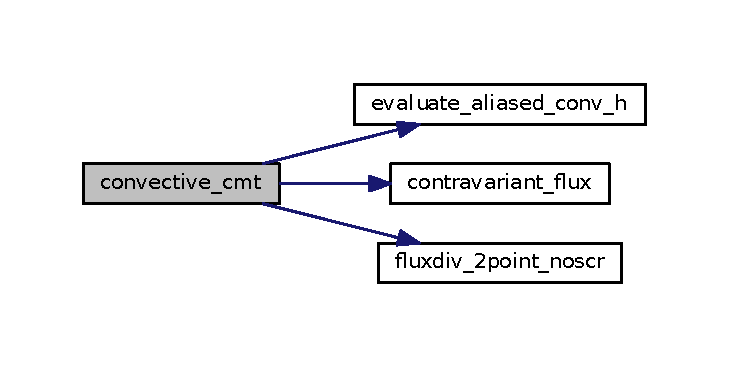
\includegraphics[width=350pt]{group__convhvol_ga77e7d7a46950fcbbf072e8e900cee272_cgraph}
\end{center}
\end{figure}


\hypertarget{group__convhvol_gad9d70d83f1184d25495812d637698102}{\index{Volume integral for inviscid fluxes@{Volume integral for inviscid fluxes}!evaluate\-\_\-aliased\-\_\-conv\-\_\-h@{evaluate\-\_\-aliased\-\_\-conv\-\_\-h}}
\index{evaluate\-\_\-aliased\-\_\-conv\-\_\-h@{evaluate\-\_\-aliased\-\_\-conv\-\_\-h}!Volume integral for inviscid fluxes@{Volume integral for inviscid fluxes}}
\subsubsection[{evaluate\-\_\-aliased\-\_\-conv\-\_\-h}]{\setlength{\rightskip}{0pt plus 5cm}subroutine evaluate\-\_\-aliased\-\_\-conv\-\_\-h (
\begin{DoxyParamCaption}
\item[{integer}]{e}
\end{DoxyParamCaption}
)}}\label{group__convhvol_gad9d70d83f1184d25495812d637698102}


Evaluates consistent (i.\-e. $F^{\#}(U_{i,j,k},U_{l,j,k})=H_{(eq),i},i=l$) flux function at all G\-L\-L nodes and stores it in convh. 


\begin{DoxyParams}{Parameters}
{\em e} & integer index of the element (intent(in)) \\
\hline
\end{DoxyParams}
\hypertarget{group__convhvol_ga72c1cbe51bc537e14ec8927e62f0e3f3}{\index{Volume integral for inviscid fluxes@{Volume integral for inviscid fluxes}!fluxdiv\-\_\-2point\-\_\-noscr@{fluxdiv\-\_\-2point\-\_\-noscr}}
\index{fluxdiv\-\_\-2point\-\_\-noscr@{fluxdiv\-\_\-2point\-\_\-noscr}!Volume integral for inviscid fluxes@{Volume integral for inviscid fluxes}}
\subsubsection[{fluxdiv\-\_\-2point\-\_\-noscr}]{\setlength{\rightskip}{0pt plus 5cm}subroutine fluxdiv\-\_\-2point\-\_\-noscr (
\begin{DoxyParamCaption}
\item[{real, dimension(lx1,ly1,lz1,lelt,toteq)}]{res, }
\item[{real, dimension(lx1,ly1,lz1,3,toteq)}]{fcons, }
\item[{integer}]{e, }
\item[{real, dimension(lx1,ly1,lz1,ldim,ldim)}]{ja}
\end{DoxyParamCaption}
)}}\label{group__convhvol_ga72c1cbe51bc537e14ec8927e62f0e3f3}


Evaluates the two-\/point split form (Equations~\ref{splitr} through ~\ref{splitt}) of the volume integral $\int v \nabla\cdot\mathbf{H}^c dV$ and the discontinuous surface flux $\oint v \mathbf{H}^c\cdot\mathbf{n} dA$ for the inviscid flux function in a single element. 


\begin{DoxyParams}{Parameters}
{\em res} & R\-H\-S for all equations, all elements (intent(inout))\\
\hline
{\em ja} & Metrics for the e'th elements (intent(in))\\
\hline
{\em fcons} & Consistent contravariant flux $Jdiag\left(\partial r_i/\partial x_k\right) \bH_k$ (intent(in)) \\
\hline
\end{DoxyParams}
Both $\int v \nabla\cdot\mathbf{H}^c dV$ and flux $\oint v \mathbf{H}^c\cdot\mathbf{n} dA$ for the inviscid flux are added to res1 for the element $e$. The volume integrand is approximated by $\sum D_{il} F^{\#}(z_{i,j,k},z_{l,j,k})$ in each of the ndim directions of the reference element. The two-\/point flux function $F^{\#}(z_1,z_2)$ is taken from \hyperlink{fluxfn_8f}{fluxfn.\-f} and specified in the usr file in cmt\-\_\-usr2pt.

The parameter vector $z$ is computed from primitive variables in element $e$ of S\-O\-L\-N and stored one element at a time in /scrns/ zaux according to cmt\-\_\-usrz. $U$ is transposed and stored for element $e$ in ut.\hypertarget{group__convhvol_gab4831bb28a78e1c8fd3ec09854bd15ad}{\index{Volume integral for inviscid fluxes@{Volume integral for inviscid fluxes}!fluxdiv\-\_\-strong\-\_\-contra@{fluxdiv\-\_\-strong\-\_\-contra}}
\index{fluxdiv\-\_\-strong\-\_\-contra@{fluxdiv\-\_\-strong\-\_\-contra}!Volume integral for inviscid fluxes@{Volume integral for inviscid fluxes}}
\subsubsection[{fluxdiv\-\_\-strong\-\_\-contra}]{\setlength{\rightskip}{0pt plus 5cm}subroutine fluxdiv\-\_\-strong\-\_\-contra (
\begin{DoxyParamCaption}
\item[{integer}]{e}
\end{DoxyParamCaption}
)}}\label{group__convhvol_gab4831bb28a78e1c8fd3ec09854bd15ad}


Computes $\int v \nabla\cdot\mathbf{H}^c dV$ in aliased strong form for element $e$, and increments res1 with it. 


\begin{DoxyParams}{Parameters}
{\em e} & integer index of the element (intent(in)) \\
\hline
\end{DoxyParams}

\hypertarget{group__bcond}{\section{Surface integrals due to boundary conditions}
\label{group__bcond}\index{Surface integrals due to boundary conditions@{Surface integrals due to boundary conditions}}
}
\subsection*{Functions/\-Subroutines}
\begin{DoxyCompactItemize}
\item 
\hypertarget{group__bcond_ga45475eec850fc7ef33c51a25b4f86602}{subroutine \hyperlink{group__bcond_ga45475eec850fc7ef33c51a25b4f86602}{inviscidbc} (flux)}\label{group__bcond_ga45475eec850fc7ef33c51a25b4f86602}

\begin{DoxyCompactList}\small\item\em Determining rind state for Dirichlet boundary conditions. \end{DoxyCompactList}\item 
\hypertarget{group__bcond_ga917af547cc29afcf40e2b54c6a97c90d}{subroutine \hyperlink{group__bcond_ga917af547cc29afcf40e2b54c6a97c90d}{bcmask\-\_\-cmt} (bmsk)}\label{group__bcond_ga917af547cc29afcf40e2b54c6a97c90d}

\begin{DoxyCompactList}\small\item\em Mask to make sure Fsharp doesn't clobber boundary faces, where gs\-\_\-op is null This routine intents to take a real array for all face points, bmask, and only zero out faces on boundaries. It is thus not limited to an array only of indicators. \end{DoxyCompactList}\item 
\hypertarget{group__bcond_ga73b8f242bb8ea95b0c7baf512eeac825}{subroutine \hyperlink{group__bcond_ga73b8f242bb8ea95b0c7baf512eeac825}{bcflux} (flux, \hyperlink{group__vfjac_ga9087d56c6c467d3ffeb9aa6be3f43e82}{agradu}, qminus)}\label{group__bcond_ga73b8f242bb8ea95b0c7baf512eeac825}

\begin{DoxyCompactList}\small\item\em Determining I\-G\-U contribution to boundary flux. 0 for artificial viscosity, and strictly interior for physical viscosity. \end{DoxyCompactList}\item 
\hypertarget{group__bcond_ga9a5825c588243a1c261d107376f5a873}{subroutine \hyperlink{group__bcond_ga9a5825c588243a1c261d107376f5a873}{a5adiabatic\-\_\-wall} (eflx, f, e, d\-U, wstate)}\label{group__bcond_ga9a5825c588243a1c261d107376f5a873}

\begin{DoxyCompactList}\small\item\em computes boundary flux for adiabatic wall in igu \end{DoxyCompactList}\item 
subroutine \hyperlink{group__bcond_ga224b6cf6476419f057df67c7a0d05504}{a51duadia} (flux, f, ie, d\-U, wstate)
\begin{DoxyCompactList}\small\item\em same as A51 for volume flux (x-\/direction viscous flux of energy, but \end{DoxyCompactList}\item 
subroutine \hyperlink{group__bcond_gaaaddd14c010da1bce6192846a45b63f2}{a52duadia} (flux, f, ie, d\-U, wstate)
\begin{DoxyCompactList}\small\item\em same as A51 for volume flux (y-\/direction viscous flux of energy, but \end{DoxyCompactList}\item 
subroutine \hyperlink{group__bcond_ga4311cb4d64847bc8b17c653ca9185866}{a53duadia} (flux, f, ie, d\-U, wstate)
\begin{DoxyCompactList}\small\item\em same as A51 for volume flux (z-\/direction viscous flux of energy, but \end{DoxyCompactList}\item 
subroutine \hyperlink{group__bcond_ga01708cdee955465babb7a371d4e5effa}{imqqtu\-\_\-dirichlet} (umubc, wminus, wplus)
\begin{DoxyCompactList}\small\item\em $\left(\mathbf{I}-1/2QQ^T\right)\mathbf{U}\rightarrow\mathbf{U}^--\mathbf{U}^D$ on Dirichlet boundaries. Currently only modifies $\mathbf{U}^+$ in the case of walls. \end{DoxyCompactList}\end{DoxyCompactItemize}


\subsection{Detailed Description}


\subsection{Function/\-Subroutine Documentation}
\hypertarget{group__bcond_ga224b6cf6476419f057df67c7a0d05504}{\index{Surface integrals due to boundary conditions@{Surface integrals due to boundary conditions}!a51duadia@{a51duadia}}
\index{a51duadia@{a51duadia}!Surface integrals due to boundary conditions@{Surface integrals due to boundary conditions}}
\subsubsection[{a51duadia}]{\setlength{\rightskip}{0pt plus 5cm}subroutine a51duadia (
\begin{DoxyParamCaption}
\item[{real, dimension  (lx1$\ast$ly1$\ast$lz1)}]{flux, }
\item[{integer}]{f, }
\item[{}]{ie, }
\item[{real, dimension    (lx1$\ast$lz1,2$\ast$ldim,nelt,toteq,3)}]{d\-U, }
\item[{real, dimension(lx1$\ast$lz1,2$\ast$ldim,nelt,nqq)}]{wstate}
\end{DoxyParamCaption}
)}}\label{group__bcond_ga224b6cf6476419f057df67c7a0d05504}


same as A51 for volume flux (x-\/direction viscous flux of energy, but 


\begin{DoxyEnumerate}
\item uses wstate for contiguous storage of data on faces.
\item locally sets K=0 to prevent heat transfer through adiabatic walls 
\end{DoxyEnumerate}\hypertarget{group__bcond_gaaaddd14c010da1bce6192846a45b63f2}{\index{Surface integrals due to boundary conditions@{Surface integrals due to boundary conditions}!a52duadia@{a52duadia}}
\index{a52duadia@{a52duadia}!Surface integrals due to boundary conditions@{Surface integrals due to boundary conditions}}
\subsubsection[{a52duadia}]{\setlength{\rightskip}{0pt plus 5cm}subroutine a52duadia (
\begin{DoxyParamCaption}
\item[{real, dimension  (lx1$\ast$ly1$\ast$lz1)}]{flux, }
\item[{integer}]{f, }
\item[{}]{ie, }
\item[{real, dimension    (lx1$\ast$lz1,2$\ast$ldim,nelt,toteq,3)}]{d\-U, }
\item[{real, dimension(lx1$\ast$lz1,2$\ast$ldim,nelt,nqq)}]{wstate}
\end{DoxyParamCaption}
)}}\label{group__bcond_gaaaddd14c010da1bce6192846a45b63f2}


same as A51 for volume flux (y-\/direction viscous flux of energy, but 


\begin{DoxyEnumerate}
\item uses wstate for contiguous storage of data on faces.
\item locally sets K=0 to prevent heat transfer through adiabatic walls 
\end{DoxyEnumerate}\hypertarget{group__bcond_ga4311cb4d64847bc8b17c653ca9185866}{\index{Surface integrals due to boundary conditions@{Surface integrals due to boundary conditions}!a53duadia@{a53duadia}}
\index{a53duadia@{a53duadia}!Surface integrals due to boundary conditions@{Surface integrals due to boundary conditions}}
\subsubsection[{a53duadia}]{\setlength{\rightskip}{0pt plus 5cm}subroutine a53duadia (
\begin{DoxyParamCaption}
\item[{real, dimension  (lx1$\ast$ly1$\ast$lz1)}]{flux, }
\item[{integer}]{f, }
\item[{}]{ie, }
\item[{real, dimension    (lx1$\ast$lz1,2$\ast$ldim,nelt,toteq,3)}]{d\-U, }
\item[{real, dimension(lx1$\ast$lz1,2$\ast$ldim,nelt,nqq)}]{wstate}
\end{DoxyParamCaption}
)}}\label{group__bcond_ga4311cb4d64847bc8b17c653ca9185866}


same as A51 for volume flux (z-\/direction viscous flux of energy, but 


\begin{DoxyEnumerate}
\item uses wstate for contiguous storage of data on faces.
\item locally sets K=0 to prevent heat transfer through adiabatic walls 
\end{DoxyEnumerate}\hypertarget{group__bcond_ga01708cdee955465babb7a371d4e5effa}{\index{Surface integrals due to boundary conditions@{Surface integrals due to boundary conditions}!imqqtu\-\_\-dirichlet@{imqqtu\-\_\-dirichlet}}
\index{imqqtu\-\_\-dirichlet@{imqqtu\-\_\-dirichlet}!Surface integrals due to boundary conditions@{Surface integrals due to boundary conditions}}
\subsubsection[{imqqtu\-\_\-dirichlet}]{\setlength{\rightskip}{0pt plus 5cm}subroutine imqqtu\-\_\-dirichlet (
\begin{DoxyParamCaption}
\item[{real, dimension (lx1$\ast$lz1,2$\ast$ldim,nelt,toteq)}]{umubc, }
\item[{real, dimension(lx1$\ast$lz1,2$\ast$ldim,nelt,nqq)}]{wminus, }
\item[{real, dimension (lx1$\ast$lz1,2$\ast$ldim,nelt,nqq)}]{wplus}
\end{DoxyParamCaption}
)}}\label{group__bcond_ga01708cdee955465babb7a371d4e5effa}


$\left(\mathbf{I}-1/2QQ^T\right)\mathbf{U}\rightarrow\mathbf{U}^--\mathbf{U}^D$ on Dirichlet boundaries. Currently only modifies $\mathbf{U}^+$ in the case of walls. 


\begin{DoxyParams}{Parameters}
{\em umubc} & $\mathbf{U}^--\mathbf{U}^D$ (intent(out))\\
\hline
{\em wminus} & interior values of primitive variables on boundary faces (intent(in))\\
\hline
{\em wplus} & exterior values of primitive variables on faces with Dirichlet B\-C. Filled with desired boundary condition values (intent(inout)) on entry, but modified for adiabatic walls. \\
\hline
\end{DoxyParams}

\hypertarget{group__diffhvol}{\section{Volume integral for viscous fluxes}
\label{group__diffhvol}\index{Volume integral for viscous fluxes@{Volume integral for viscous fluxes}}
}
\subsection*{Functions/\-Subroutines}
\begin{DoxyCompactItemize}
\item 
subroutine \hyperlink{group__diffhvol_ga90ef567419c8aa503af50a7e747c884e}{half\-\_\-iku\-\_\-cmt} (res, diffh, e)
\begin{DoxyCompactList}\small\item\em Compute the integrand $\mathbf{D}^{T}\mathbf{H}^d$ of the weak-\/form volume integral and store it in res1 one element per call. \end{DoxyCompactList}\item 
subroutine \hyperlink{group__diffhvol_ga6d611a250fb98acf77e8a3880c0e608d}{viscous\-\_\-cmt} (e, eq)
\begin{DoxyCompactList}\small\item\em Volume integral for diffusive terms. \end{DoxyCompactList}\end{DoxyCompactItemize}


\subsection{Detailed Description}


\subsection{Function/\-Subroutine Documentation}
\hypertarget{group__diffhvol_ga90ef567419c8aa503af50a7e747c884e}{\index{Volume integral for viscous fluxes@{Volume integral for viscous fluxes}!half\-\_\-iku\-\_\-cmt@{half\-\_\-iku\-\_\-cmt}}
\index{half\-\_\-iku\-\_\-cmt@{half\-\_\-iku\-\_\-cmt}!Volume integral for viscous fluxes@{Volume integral for viscous fluxes}}
\subsubsection[{half\-\_\-iku\-\_\-cmt}]{\setlength{\rightskip}{0pt plus 5cm}subroutine half\-\_\-iku\-\_\-cmt (
\begin{DoxyParamCaption}
\item[{real, dimension(lx1,ly1,lz1)}]{res, }
\item[{real, dimension(lx1$\ast$ly1$\ast$lz1,ldim)}]{diffh, }
\item[{integer}]{e}
\end{DoxyParamCaption}
)}}\label{group__diffhvol_ga90ef567419c8aa503af50a7e747c884e}


Compute the integrand $\mathbf{D}^{T}\mathbf{H}^d$ of the weak-\/form volume integral and store it in res1 one element per call. 


\begin{DoxyParams}{Parameters}
{\em e} & index of element under consideration (intent(in))\\
\hline
{\em res} & res+= $\mathbf{D}^{T}\mathbf{H}^{(d)}$. Actual argument is a single element of res1 for a single equation (intent(inout))\\
\hline
{\em diffh} & viscous flux $\mathbf{H}^{(d)}$ for a single element and single equation. Overwritten (intent(inout)) \\
\hline
\end{DoxyParams}
$\mathbf{M}\mathbf{H}^d$ in diffh

$\mathbf{D}^{T}\mathbf{M}\mathbf{H}^d$ in rscr for element $e$.

$\mathbf{M}^{-1}\mathbf{D}^{T}\mathbf{M}\mathbf{H}^d$ in rscr for element $e$.

add rscr to res\hypertarget{group__diffhvol_ga6d611a250fb98acf77e8a3880c0e608d}{\index{Volume integral for viscous fluxes@{Volume integral for viscous fluxes}!viscous\-\_\-cmt@{viscous\-\_\-cmt}}
\index{viscous\-\_\-cmt@{viscous\-\_\-cmt}!Volume integral for viscous fluxes@{Volume integral for viscous fluxes}}
\subsubsection[{viscous\-\_\-cmt}]{\setlength{\rightskip}{0pt plus 5cm}subroutine viscous\-\_\-cmt (
\begin{DoxyParamCaption}
\item[{integer}]{e, }
\item[{integer}]{eq}
\end{DoxyParamCaption}
)}}\label{group__diffhvol_ga6d611a250fb98acf77e8a3880c0e608d}


Volume integral for diffusive terms. 

Compute $\mathbf{H}^d=A\nabla U$ and store it in diffh for element $e$.

Store faces of $\mathbf{H}^d$ in /\-C\-M\-T\-S\-U\-R\-F\-L\-X/ for $\mathbf{I}_{GU}$ or B\-R1.

Compute the integrand $\mathbf{D}^{T}\mathbf{H}^d$ of the weak-\/form volume integral and store it in res1.

Here is the call graph for this function\-:\nopagebreak
\begin{figure}[H]
\begin{center}
\leavevmode
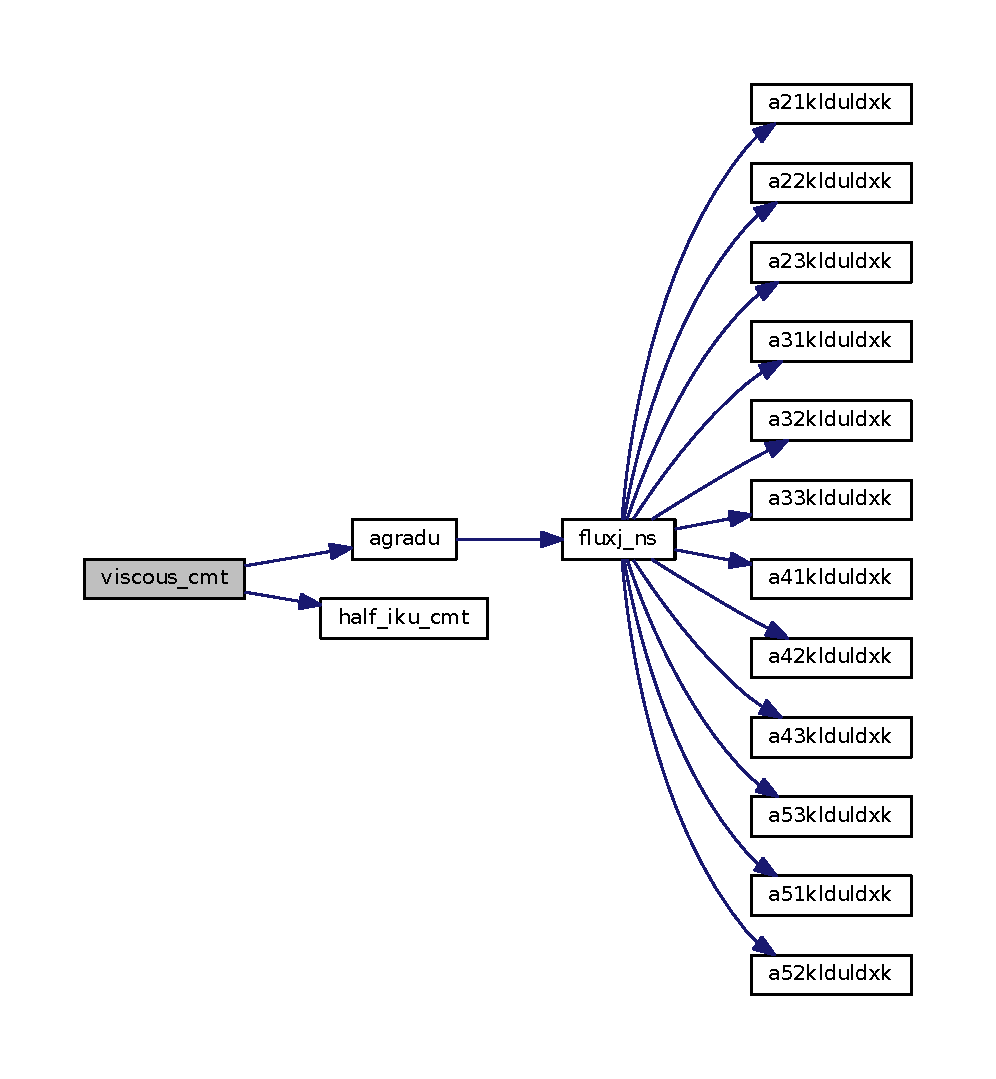
\includegraphics[width=350pt]{group__diffhvol_ga6d611a250fb98acf77e8a3880c0e608d_cgraph}
\end{center}
\end{figure}



\hypertarget{group__vfjac}{\section{Jacobians for viscous fluxes}
\label{group__vfjac}\index{Jacobians for viscous fluxes@{Jacobians for viscous fluxes}}
}
\subsection*{Functions/\-Subroutines}
\begin{DoxyCompactItemize}
\item 
subroutine \hyperlink{group__vfjac_ga9087d56c6c467d3ffeb9aa6be3f43e82}{agradu} (flux, du, e, eq)
\begin{DoxyCompactList}\small\item\em Transforms the gradients of conserved variables $\nabla \mathbf{U}$ to the viscous flux $\mathbf{H}^{(d)}$ in a single element for a single equation. Particular choice of viscous stress tensor is currently hardcoded for Navier-\/\-Stokes. \end{DoxyCompactList}\item 
subroutine \hyperlink{group__vfjac_ga2c0d85531a9af69b9d464571ca530e5d}{fluxj\-\_\-ns} (flux, gradu, e, eq)
\begin{DoxyCompactList}\small\item\em $ \tau_{ij}=2 \mu\sigma_{ij} + \lambda \Delta \delta_{ij}$ Navier-\/\-Stokes. uservp provides properties stored in S\-O\-L\-N. Implemented via maxima-\/generated code. \end{DoxyCompactList}\item 
subroutine \hyperlink{group__vfjac_ga15f8f8f0e3d305dc065f004aa09de57c}{compute\-\_\-transport\-\_\-props}
\begin{DoxyCompactList}\small\item\em Fill vdiff with transport properties. Hardcoded indices for Navier-\/\-Stokes Used for both artificial and physical viscosities. \end{DoxyCompactList}\item 
\hypertarget{group__vfjac_ga34cccfbb67ddce8c68e7f2742a94af96}{subroutine \hyperlink{group__vfjac_ga34cccfbb67ddce8c68e7f2742a94af96}{a51klduldxk} (flux, d\-U, ie)}\label{group__vfjac_ga34cccfbb67ddce8c68e7f2742a94af96}

\begin{DoxyCompactList}\small\item\em W\-R\-I\-T\-E O\-U\-T N\-O\-T\-A\-T\-I\-O\-N. \end{DoxyCompactList}\item 
\hypertarget{group__vfjac_gad8d6f5b90772f9f1082fba425cece421}{subroutine \hyperlink{group__vfjac_gad8d6f5b90772f9f1082fba425cece421}{a52klduldxk} (flux, d\-U, ie)}\label{group__vfjac_gad8d6f5b90772f9f1082fba425cece421}

\begin{DoxyCompactList}\small\item\em W\-R\-I\-T\-E O\-U\-T N\-O\-T\-A\-T\-I\-O\-N. \end{DoxyCompactList}\item 
\hypertarget{group__vfjac_ga68680b2ed51dce76ed38535fee8c7f63}{subroutine \hyperlink{group__vfjac_ga68680b2ed51dce76ed38535fee8c7f63}{a53klduldxk} (flux, d\-U, ie)}\label{group__vfjac_ga68680b2ed51dce76ed38535fee8c7f63}

\begin{DoxyCompactList}\small\item\em W\-R\-I\-T\-E O\-U\-T N\-O\-T\-A\-T\-I\-O\-N. \end{DoxyCompactList}\item 
\hypertarget{group__vfjac_ga7818a3a1981f80b10cfc4f1d93d5babc}{subroutine \hyperlink{group__vfjac_ga7818a3a1981f80b10cfc4f1d93d5babc}{a21klduldxk} (flux, d\-U, ie)}\label{group__vfjac_ga7818a3a1981f80b10cfc4f1d93d5babc}

\begin{DoxyCompactList}\small\item\em W\-R\-I\-T\-E O\-U\-T N\-O\-T\-A\-T\-I\-O\-N. \end{DoxyCompactList}\item 
\hypertarget{group__vfjac_ga608f83273074946557a9015117c11670}{subroutine \hyperlink{group__vfjac_ga608f83273074946557a9015117c11670}{a22klduldxk} (flux, d\-U, ie)}\label{group__vfjac_ga608f83273074946557a9015117c11670}

\begin{DoxyCompactList}\small\item\em W\-R\-I\-T\-E O\-U\-T N\-O\-T\-A\-T\-I\-O\-N. \end{DoxyCompactList}\item 
\hypertarget{group__vfjac_ga9271a9b027c374b2b2fba0f7f0e00a1e}{subroutine \hyperlink{group__vfjac_ga9271a9b027c374b2b2fba0f7f0e00a1e}{a23klduldxk} (flux, d\-U, ie)}\label{group__vfjac_ga9271a9b027c374b2b2fba0f7f0e00a1e}

\begin{DoxyCompactList}\small\item\em W\-R\-I\-T\-E O\-U\-T N\-O\-T\-A\-T\-I\-O\-N. \end{DoxyCompactList}\item 
\hypertarget{group__vfjac_ga3485906a061442ec51929856cc8f4d4a}{subroutine \hyperlink{group__vfjac_ga3485906a061442ec51929856cc8f4d4a}{a31klduldxk} (flux, d\-U, ie)}\label{group__vfjac_ga3485906a061442ec51929856cc8f4d4a}

\begin{DoxyCompactList}\small\item\em W\-R\-I\-T\-E O\-U\-T N\-O\-T\-A\-T\-I\-O\-N. \end{DoxyCompactList}\item 
\hypertarget{group__vfjac_ga2a280e4b1d5fbba00356ca9120709fa0}{subroutine \hyperlink{group__vfjac_ga2a280e4b1d5fbba00356ca9120709fa0}{a32klduldxk} (flux, d\-U, ie)}\label{group__vfjac_ga2a280e4b1d5fbba00356ca9120709fa0}

\begin{DoxyCompactList}\small\item\em W\-R\-I\-T\-E O\-U\-T N\-O\-T\-A\-T\-I\-O\-N. \end{DoxyCompactList}\item 
\hypertarget{group__vfjac_ga4b542714fa89c4288fa5846a11cc28b1}{subroutine \hyperlink{group__vfjac_ga4b542714fa89c4288fa5846a11cc28b1}{a33klduldxk} (flux, d\-U, ie)}\label{group__vfjac_ga4b542714fa89c4288fa5846a11cc28b1}

\begin{DoxyCompactList}\small\item\em W\-R\-I\-T\-E O\-U\-T N\-O\-T\-A\-T\-I\-O\-N. \end{DoxyCompactList}\item 
\hypertarget{group__vfjac_ga8b5ee49aa820086e3596a1a91e9dc799}{subroutine \hyperlink{group__vfjac_ga8b5ee49aa820086e3596a1a91e9dc799}{a41klduldxk} (flux, d\-U, ie)}\label{group__vfjac_ga8b5ee49aa820086e3596a1a91e9dc799}

\begin{DoxyCompactList}\small\item\em W\-R\-I\-T\-E O\-U\-T N\-O\-T\-A\-T\-I\-O\-N. \end{DoxyCompactList}\item 
\hypertarget{group__vfjac_ga7cf0c00202b223c51bed9c61c7937bc6}{subroutine \hyperlink{group__vfjac_ga7cf0c00202b223c51bed9c61c7937bc6}{a42klduldxk} (flux, d\-U, ie)}\label{group__vfjac_ga7cf0c00202b223c51bed9c61c7937bc6}

\begin{DoxyCompactList}\small\item\em W\-R\-I\-T\-E O\-U\-T N\-O\-T\-A\-T\-I\-O\-N. \end{DoxyCompactList}\item 
\hypertarget{group__vfjac_ga7d4c71aaaae94de9cd5f41a93836699a}{subroutine \hyperlink{group__vfjac_ga7d4c71aaaae94de9cd5f41a93836699a}{a43klduldxk} (flux, d\-U, ie)}\label{group__vfjac_ga7d4c71aaaae94de9cd5f41a93836699a}

\begin{DoxyCompactList}\small\item\em W\-R\-I\-T\-E O\-U\-T N\-O\-T\-A\-T\-I\-O\-N. \end{DoxyCompactList}\end{DoxyCompactItemize}


\subsection{Detailed Description}


\subsection{Function/\-Subroutine Documentation}
\hypertarget{group__vfjac_ga9087d56c6c467d3ffeb9aa6be3f43e82}{\index{Jacobians for viscous fluxes@{Jacobians for viscous fluxes}!agradu@{agradu}}
\index{agradu@{agradu}!Jacobians for viscous fluxes@{Jacobians for viscous fluxes}}
\subsubsection[{agradu}]{\setlength{\rightskip}{0pt plus 5cm}subroutine agradu (
\begin{DoxyParamCaption}
\item[{real, dimension(lx1$\ast$ly1$\ast$lz1,ldim)}]{flux, }
\item[{real, dimension(lx1$\ast$ly1$\ast$lz1,3,toteq)}]{du, }
\item[{integer}]{e, }
\item[{integer}]{eq}
\end{DoxyParamCaption}
)}}\label{group__vfjac_ga9087d56c6c467d3ffeb9aa6be3f43e82}


Transforms the gradients of conserved variables $\nabla \mathbf{U}$ to the viscous flux $\mathbf{H}^{(d)}$ in a single element for a single equation. Particular choice of viscous stress tensor is currently hardcoded for Navier-\/\-Stokes. 


\begin{DoxyParams}{Parameters}
{\em e} & index of element for primitive variables within different flux jacobians (intent(in))\\
\hline
{\em eq} & index of conserved variable whose viscous flux is being computed. (intent(in))\\
\hline
{\em du} & gradient of conserved variables $\partial U_i/\partial x_j$ (intent(in))\\
\hline
{\em flux} & flux = $\mathbf{H}^{(d)}=\mathscr{A}\nabla \mathbf{U}$ (intent(out)) \\
\hline
\end{DoxyParams}


Here is the call graph for this function\-:\nopagebreak
\begin{figure}[H]
\begin{center}
\leavevmode
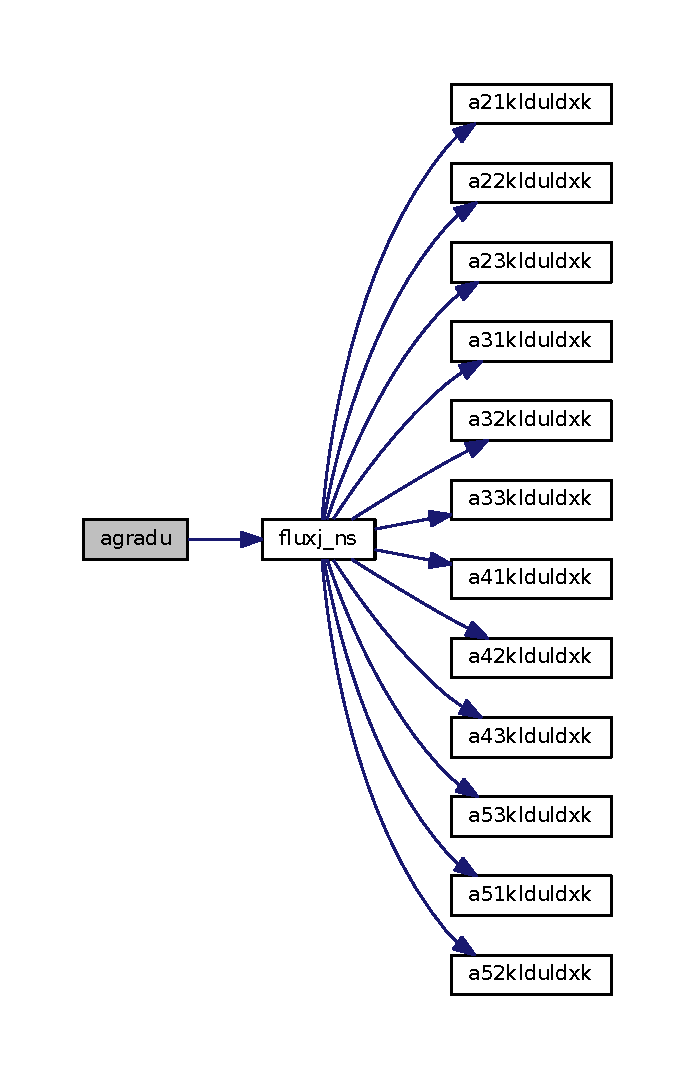
\includegraphics[width=334pt]{group__vfjac_ga9087d56c6c467d3ffeb9aa6be3f43e82_cgraph}
\end{center}
\end{figure}


\hypertarget{group__vfjac_ga15f8f8f0e3d305dc065f004aa09de57c}{\index{Jacobians for viscous fluxes@{Jacobians for viscous fluxes}!compute\-\_\-transport\-\_\-props@{compute\-\_\-transport\-\_\-props}}
\index{compute\-\_\-transport\-\_\-props@{compute\-\_\-transport\-\_\-props}!Jacobians for viscous fluxes@{Jacobians for viscous fluxes}}
\subsubsection[{compute\-\_\-transport\-\_\-props}]{\setlength{\rightskip}{0pt plus 5cm}subroutine compute\-\_\-transport\-\_\-props (
\begin{DoxyParamCaption}
{}
\end{DoxyParamCaption}
)}}\label{group__vfjac_ga15f8f8f0e3d305dc065f004aa09de57c}


Fill vdiff with transport properties. Hardcoded indices for Navier-\/\-Stokes Used for both artificial and physical viscosities. 

Indexes the element inside S\-O\-L\-N (intent(in))

Here is the call graph for this function\-:\nopagebreak
\begin{figure}[H]
\begin{center}
\leavevmode
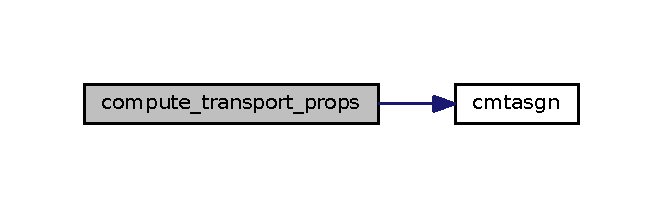
\includegraphics[width=318pt]{group__vfjac_ga15f8f8f0e3d305dc065f004aa09de57c_cgraph}
\end{center}
\end{figure}


\hypertarget{group__vfjac_ga2c0d85531a9af69b9d464571ca530e5d}{\index{Jacobians for viscous fluxes@{Jacobians for viscous fluxes}!fluxj\-\_\-ns@{fluxj\-\_\-ns}}
\index{fluxj\-\_\-ns@{fluxj\-\_\-ns}!Jacobians for viscous fluxes@{Jacobians for viscous fluxes}}
\subsubsection[{fluxj\-\_\-ns}]{\setlength{\rightskip}{0pt plus 5cm}subroutine fluxj\-\_\-ns (
\begin{DoxyParamCaption}
\item[{real, dimension(lx1$\ast$ly1$\ast$lz1,ldim)}]{flux, }
\item[{real, dimension(lx1$\ast$ly1$\ast$lz1,3,toteq)}]{gradu, }
\item[{integer}]{e, }
\item[{integer}]{eq}
\end{DoxyParamCaption}
)}}\label{group__vfjac_ga2c0d85531a9af69b9d464571ca530e5d}


$ \tau_{ij}=2 \mu\sigma_{ij} + \lambda \Delta \delta_{ij}$ Navier-\/\-Stokes. uservp provides properties stored in S\-O\-L\-N. Implemented via maxima-\/generated code. 


\begin{DoxyParams}{Parameters}
{\em e} & index of element under consideration (intent(in))\\
\hline
{\em eq} & index of conserved variable whose viscous flux is being computed. (intent(in))\\
\hline
{\em flux} & flux = $\mathbf{H}^{(d)}=\mathscr{A}\nabla \mathbf{U}$ (intent(out))\\
\hline
{\em gradu} & gradient of conserved variables $\nabla \mathbf{U}$ (intent(in)) \\
\hline
\end{DoxyParams}


Here is the call graph for this function\-:\nopagebreak
\begin{figure}[H]
\begin{center}
\leavevmode
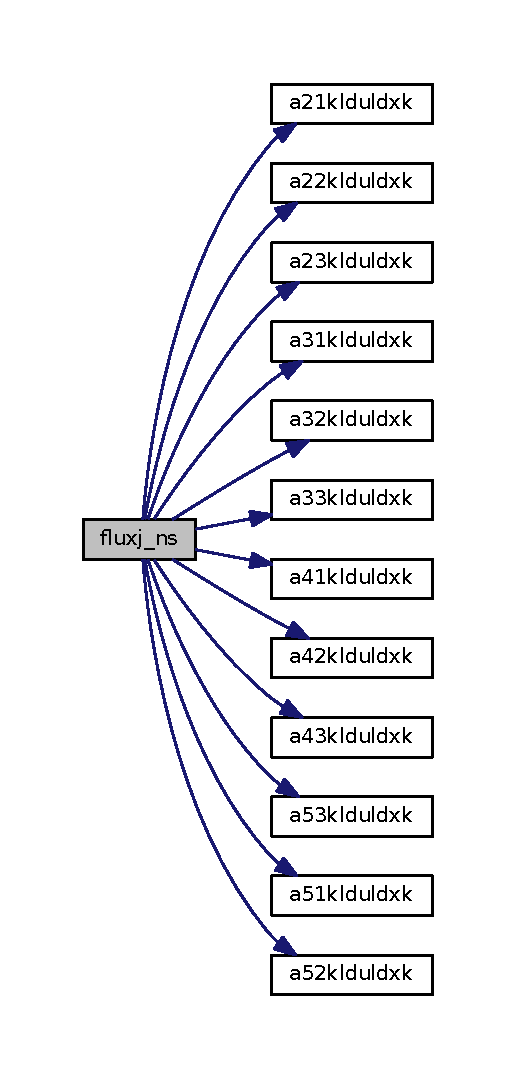
\includegraphics[width=248pt]{group__vfjac_ga2c0d85531a9af69b9d464571ca530e5d_cgraph}
\end{center}
\end{figure}



\hypertarget{group__isurf}{\section{Inviscid surface terms}
\label{group__isurf}\index{Inviscid surface terms@{Inviscid surface terms}}
}
\subsection*{Functions/\-Subroutines}
\begin{DoxyCompactItemize}
\item 
\hypertarget{group__isurf_ga2b8162e02f3f2266c59f717fa1363226}{subroutine \hyperlink{group__isurf_ga2b8162e02f3f2266c59f717fa1363226}{ausm\-\_\-fluxfunction} (ntot, nx, ny, nz, nm, fs, rl, ul, vl, wl, pl, al, tl, rr, ur, vr, wr, pr, ar, tr, flx, el, er)}\label{group__isurf_ga2b8162e02f3f2266c59f717fa1363226}

\begin{DoxyCompactList}\small\item\em Computes inviscid numerical surface flux from A\-U\-S\-M+ Riemann solver. \end{DoxyCompactList}\item 
subroutine \hyperlink{group__isurf_ga15e4fb7f0dbe0767ef81c6b291f611cb}{inflow\-\_\-df} (f, e, wm, wp, um, up, nvar)
\begin{DoxyCompactList}\small\item\em more conventional Dolejsi \& Feistauer (2015) Section 8.\-3.\-2.\-2 ``physical'' boundary conditions. Also encountered in Hartmann \& Houston (2006). A poor default. \end{DoxyCompactList}\item 
subroutine \hyperlink{group__isurf_ga0293ec162f23a55a9e89cf0797cbf2b2}{outflow\-\_\-df} (f, e, wm, wp, um, up, nvar)
\begin{DoxyCompactList}\small\item\em Dolejsi \& Feistauer (2015) Section 8.\-3.\-2.\-2. Very rudimentary ``physical'' boundary conditions. Also encountered in Hartmann \& Houston (2006). A poor default. \end{DoxyCompactList}\item 
\hypertarget{group__isurf_gaecf15d43e4c71d130e4ef9e4a6a7821a}{subroutine \hyperlink{group__isurf_gaecf15d43e4c71d130e4ef9e4a6a7821a}{fillujumpu}}\label{group__isurf_gaecf15d43e4c71d130e4ef9e4a6a7821a}

\begin{DoxyCompactList}\small\item\em overwrite beginning of /\-C\-M\-T\-S\-U\-R\-F\-L\-X/ with $-[[\mathbf{U}]]$ for flux of auxiliary variable in the viscous flux of Bassi and Rebay computed in br1auxflux. \end{DoxyCompactList}\item 
subroutine \hyperlink{group__isurf_ga0013a607a259d0c07734b1816f8c9f60}{fluxes\-\_\-full\-\_\-field\-\_\-kg}
\begin{DoxyCompactList}\small\item\em Restrict and copy face data and compute inviscid numerical flux $\oint \mathbf{H}^{c\ast}\cdot\mathbf{n}dA$ on face points. This particular wrapper is for the symmetric flux of Kennedy and Gruber. \end{DoxyCompactList}\item 
subroutine \hyperlink{group__isurf_ga272adf58402c1bfb170c8667bf6be790}{faceu} (ivar, yourface)
\begin{DoxyCompactList}\small\item\em Restrict and copy face data for conserved variables $U_{\mbox{ivar}}$. Wraps full2face\-\_\-cmt for each element; a single call to full2face with $U$ will not work because element varies with the outermost index of the u array. \end{DoxyCompactList}\item 
subroutine \hyperlink{group__isurf_gae375bb9d6acee4eff74aa072206109a2}{fillq} (jvar, field, wminus, yourface)
\begin{DoxyCompactList}\small\item\em Restrict and copy face data for one full field and store it in index jvar in wminus. \end{DoxyCompactList}\item 
subroutine \hyperlink{group__isurf_ga317b9a948c8717ad9c64e0fae72c8641}{dg\-\_\-face\-\_\-avg} (mine, nf, nstate, handle)
\begin{DoxyCompactList}\small\item\em Overwrite values stored at points on faces with the average with its values in the neighboring face without duplication. Replaces $mine$ with $\{\{mine\}\}$. \end{DoxyCompactList}\item 
subroutine \hyperlink{group__isurf_ga53412d5d95cd62ca86dd08374a330b02}{face\-\_\-state\-\_\-commo} (mine, yours, nf, nstate, handle)
\begin{DoxyCompactList}\small\item\em Sends face values $v^-$ stored in ``mine'' to the neighbor that shares that face and copies the neighbor's values $v^+$ at each face into ``yours.''. \end{DoxyCompactList}\item 
subroutine \hyperlink{group__isurf_gaf55d5b18c1b922832898c46176f13386}{avg\-\_\-and\-\_\-jump} (avg, jump, scratch, nf, nstate, handle)
\begin{DoxyCompactList}\small\item\em Overwrites $w^-$ at interior face points stored in avg with $\{\{w\}\}$. jump gets filled with $[[w]]$. \end{DoxyCompactList}\end{DoxyCompactItemize}


\subsection{Detailed Description}


\subsection{Function/\-Subroutine Documentation}
\hypertarget{group__isurf_gaf55d5b18c1b922832898c46176f13386}{\index{Inviscid surface terms@{Inviscid surface terms}!avg\-\_\-and\-\_\-jump@{avg\-\_\-and\-\_\-jump}}
\index{avg\-\_\-and\-\_\-jump@{avg\-\_\-and\-\_\-jump}!Inviscid surface terms@{Inviscid surface terms}}
\subsubsection[{avg\-\_\-and\-\_\-jump}]{\setlength{\rightskip}{0pt plus 5cm}subroutine avg\-\_\-and\-\_\-jump (
\begin{DoxyParamCaption}
\item[{real, dimension($\ast$)}]{avg, }
\item[{real, dimension($\ast$)}]{jump, }
\item[{real, dimension($\ast$)}]{scratch, }
\item[{integer}]{nf, }
\item[{integer}]{nstate, }
\item[{integer}]{handle}
\end{DoxyParamCaption}
)}}\label{group__isurf_gaf55d5b18c1b922832898c46176f13386}


Overwrites $w^-$ at interior face points stored in avg with $\{\{w\}\}$. jump gets filled with $[[w]]$. 


\begin{DoxyParams}{Parameters}
{\em handle} & integer handle for gs\-\_\-op. needs to be set by fgslib\-\_\-gs\-\_\-setup call in setup\-\_\-cmt\-\_\-gs call (intent(in))\\
\hline
{\em nf} & Total number of face points on all faces in the domain. (intent(in), but should always be lx1$\ast$lz1$\ast$2$\ast$ldim$\ast$nelt)\\
\hline
{\em nstate} & Number of distinct fields whose copies are to be transfered between neighboring elements (intent(in))\\
\hline
{\em avg} & Real buffer (intent(inout)) $w^-$ on input, $\{\{w\}\}$ on output\\
\hline
{\em jump} & Real buffer (intent(out)) $w^-$ on input, $[[w]]$ on output\\
\hline
{\em scratch} & Real scratch (intent(out)) \\
\hline
\end{DoxyParams}
\hypertarget{group__isurf_ga317b9a948c8717ad9c64e0fae72c8641}{\index{Inviscid surface terms@{Inviscid surface terms}!dg\-\_\-face\-\_\-avg@{dg\-\_\-face\-\_\-avg}}
\index{dg\-\_\-face\-\_\-avg@{dg\-\_\-face\-\_\-avg}!Inviscid surface terms@{Inviscid surface terms}}
\subsubsection[{dg\-\_\-face\-\_\-avg}]{\setlength{\rightskip}{0pt plus 5cm}subroutine dg\-\_\-face\-\_\-avg (
\begin{DoxyParamCaption}
\item[{real, dimension($\ast$)}]{mine, }
\item[{integer}]{nf, }
\item[{integer}]{nstate, }
\item[{integer}]{handle}
\end{DoxyParamCaption}
)}}\label{group__isurf_ga317b9a948c8717ad9c64e0fae72c8641}


Overwrite values stored at points on faces with the average with its values in the neighboring face without duplication. Replaces $mine$ with $\{\{mine\}\}$. 


\begin{DoxyParams}{Parameters}
{\em handle} & integer handle for gs\-\_\-op. needs to be set by fgslib\-\_\-gs\-\_\-setup call in setup\-\_\-cmt\-\_\-gs call (intent(in))\\
\hline
{\em nf} & Total number of face points on all faces in the domain. (intent(in), but should always be lx1$\ast$lz1$\ast$2$\ast$ldim$\ast$nelt)\\
\hline
{\em nstate} & Number of distinct fields whose averages between neighboring elements are to be computed and stored at face points (intent(in))\\
\hline
{\em mine} & Buffer, but should be some large array within /\-C\-M\-T\-S\-U\-R\-F\-L\-X/ (real, intent(inout)) \\
\hline
\end{DoxyParams}
\hypertarget{group__isurf_ga53412d5d95cd62ca86dd08374a330b02}{\index{Inviscid surface terms@{Inviscid surface terms}!face\-\_\-state\-\_\-commo@{face\-\_\-state\-\_\-commo}}
\index{face\-\_\-state\-\_\-commo@{face\-\_\-state\-\_\-commo}!Inviscid surface terms@{Inviscid surface terms}}
\subsubsection[{face\-\_\-state\-\_\-commo}]{\setlength{\rightskip}{0pt plus 5cm}subroutine face\-\_\-state\-\_\-commo (
\begin{DoxyParamCaption}
\item[{real, dimension($\ast$)}]{mine, }
\item[{real, dimension($\ast$)}]{yours, }
\item[{integer}]{nf, }
\item[{integer}]{nstate, }
\item[{integer}]{handle}
\end{DoxyParamCaption}
)}}\label{group__isurf_ga53412d5d95cd62ca86dd08374a330b02}


Sends face values $v^-$ stored in ``mine'' to the neighbor that shares that face and copies the neighbor's values $v^+$ at each face into ``yours.''. 


\begin{DoxyParams}{Parameters}
{\em handle} & integer handle for gs\-\_\-op. needs to be set by fgslib\-\_\-gs\-\_\-setup call in setup\-\_\-cmt\-\_\-gs call (intent(in))\\
\hline
{\em nf} & Total number of face points on all faces in the domain. (intent(in), but should always be lx1$\ast$lz1$\ast$2$\ast$ldim$\ast$nelt)\\
\hline
{\em nstate} & Number of distinct fields whose copies are to be transfered between neighboring elements (intent(in))\\
\hline
{\em mine} & Buffer storing interior states $v^-$ in /\-C\-M\-T\-S\-U\-R\-F\-L\-X/ (real, intent(in))\\
\hline
{\em yours} & Buffer storing exterior/neighbor states $v^+$ in /\-C\-M\-T\-S\-U\-R\-F\-L\-X/ (real, intent(out)) \\
\hline
\end{DoxyParams}
\hypertarget{group__isurf_ga272adf58402c1bfb170c8667bf6be790}{\index{Inviscid surface terms@{Inviscid surface terms}!faceu@{faceu}}
\index{faceu@{faceu}!Inviscid surface terms@{Inviscid surface terms}}
\subsubsection[{faceu}]{\setlength{\rightskip}{0pt plus 5cm}subroutine faceu (
\begin{DoxyParamCaption}
\item[{integer}]{ivar, }
\item[{real, dimension(lx1,lz1,2$\ast$ldim,nelt)}]{yourface}
\end{DoxyParamCaption}
)}}\label{group__isurf_ga272adf58402c1bfb170c8667bf6be790}


Restrict and copy face data for conserved variables $U_{\mbox{ivar}}$. Wraps full2face\-\_\-cmt for each element; a single call to full2face with $U$ will not work because element varies with the outermost index of the u array. 


\begin{DoxyParams}{Parameters}
{\em ivar} & index of variable within U. ivar=1 for $\phi\rho$, ivar=2-\/4 for $\phi\rho u_i$, etc.\\
\hline
{\em yourface} & contiguous pile of faces for the $ivar^{th}$ conserved variable. (dimension(lx1,lz1,2$\ast$ldim,nelt), intent(out)) \\
\hline
\end{DoxyParams}
\hypertarget{group__isurf_gae375bb9d6acee4eff74aa072206109a2}{\index{Inviscid surface terms@{Inviscid surface terms}!fillq@{fillq}}
\index{fillq@{fillq}!Inviscid surface terms@{Inviscid surface terms}}
\subsubsection[{fillq}]{\setlength{\rightskip}{0pt plus 5cm}subroutine fillq (
\begin{DoxyParamCaption}
\item[{integer}]{jvar, }
\item[{real, dimension(lx1,ly1,lz1,nelt)}]{field, }
\item[{real, dimension(lx1$\ast$lz1$\ast$2$\ast$ldim$\ast$nelt,$\ast$)}]{wminus, }
\item[{real, dimension(lx1$\ast$lz1$\ast$2$\ast$ldim$\ast$nelt)}]{yourface}
\end{DoxyParamCaption}
)}}\label{group__isurf_gae375bb9d6acee4eff74aa072206109a2}


Restrict and copy face data for one full field and store it in index jvar in wminus. 


\begin{DoxyParams}{Parameters}
{\em jvar} & index within wminus where field array at points lying on faces will be stored (intent(in))\\
\hline
{\em field} & full array of values at each G\-L\-L point in all elements (intent(in), dimension(lx1,ly1,lz1,nelt))\\
\hline
{\em wminus} & contiguous storage for multiple fields at all G\-L\-L nodes lying on faces of each element (intent(out), dimension(lx1$\ast$lz1$\ast$2$\ast$ldim$\ast$nelt,$\ast$))\\
\hline
{\em yourface} & contiguous scratch array for a single field at all G\-L\-L nodes lying on faces of each element (intent(out), dimension(lx1$\ast$lz1$\ast$2$\ast$ldim$\ast$nelt)) \\
\hline
\end{DoxyParams}
\hypertarget{group__isurf_ga0013a607a259d0c07734b1816f8c9f60}{\index{Inviscid surface terms@{Inviscid surface terms}!fluxes\-\_\-full\-\_\-field\-\_\-kg@{fluxes\-\_\-full\-\_\-field\-\_\-kg}}
\index{fluxes\-\_\-full\-\_\-field\-\_\-kg@{fluxes\-\_\-full\-\_\-field\-\_\-kg}!Inviscid surface terms@{Inviscid surface terms}}
\subsubsection[{fluxes\-\_\-full\-\_\-field\-\_\-kg}]{\setlength{\rightskip}{0pt plus 5cm}subroutine fluxes\-\_\-full\-\_\-field\-\_\-kg (
\begin{DoxyParamCaption}
{}
\end{DoxyParamCaption}
)}}\label{group__isurf_ga0013a607a259d0c07734b1816f8c9f60}


Restrict and copy face data and compute inviscid numerical flux $\oint \mathbf{H}^{c\ast}\cdot\mathbf{n}dA$ on face points. This particular wrapper is for the symmetric flux of Kennedy and Gruber. 

\char`\"{}heresize\char`\"{} and \char`\"{}hdsize\char`\"{} come from a failed attempt at managing memory in C\-M\-T\-S\-U\-R\-F\-L\-X by redeclaration that was abandoned before the two-\/point split form. They need to be taken care of in C\-M\-T\-S\-I\-Z\-E and consistent with the desired subroutine

duplicate one conserved variable (from neighboring elements) at a time for jumps in L\-L\-F

store it before phi, which lives at jph=nqq

Stabilization first. Local Lax Friedrichs for equations 1 through 4 (mass \& momentum)

O\-N\-L\-Y needed by Kennedy-\/\-Gruber (2008) as written. This is done in fstab for Chandrashekar (2013), but overwrites jsnd for K\-G and friends.

$\mathbf{q}^- \rightarrow \mathbf{z}^-$. Kennedy-\/\-Gruber, Pirozzoli, and most energy-\/ conserving fluxes have $\mathbf{z}=\mathbf{q}$, so I just divide total energy by $U_1$ here since Kennedy-\/\-Gruber needs $E$.

$\mathbf{z}^- \rightarrow \hat{z}^-$, which is $\{\{\mathbf{z}\}\}$ for Kennedy-\/\-Gruber, Pirozzoli, and some parts of other energy-\/conserving fluxes.

$\hat{z} \rightarrow F^{\#}$. Some parameter-\/vector stuff can go here too as long as it's all local to a given element.

Now do all fluxes for all boundaries, both $F^{\#}$ and stabilized

Here is the call graph for this function\-:\nopagebreak
\begin{figure}[H]
\begin{center}
\leavevmode
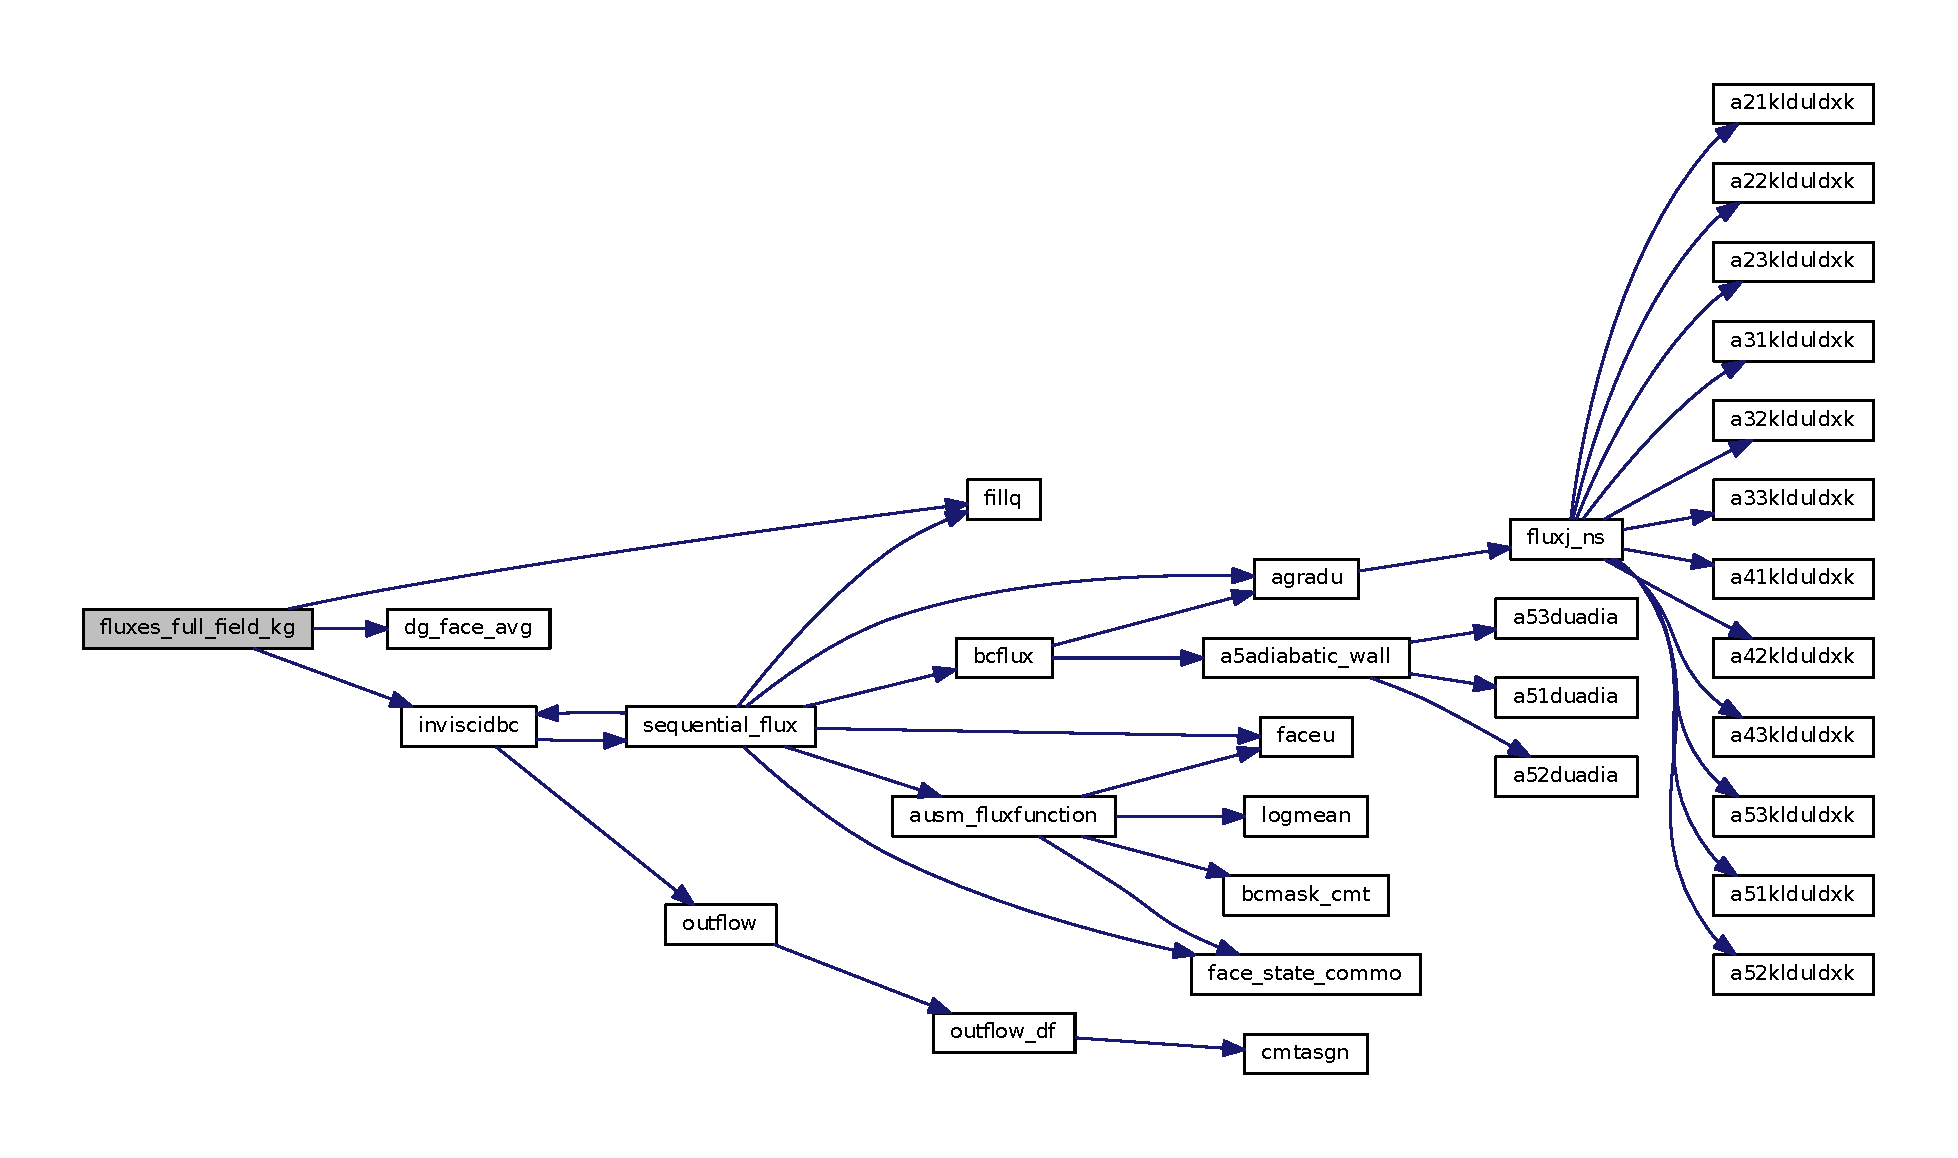
\includegraphics[width=350pt]{group__isurf_ga0013a607a259d0c07734b1816f8c9f60_cgraph}
\end{center}
\end{figure}


\hypertarget{group__isurf_ga15e4fb7f0dbe0767ef81c6b291f611cb}{\index{Inviscid surface terms@{Inviscid surface terms}!inflow\-\_\-df@{inflow\-\_\-df}}
\index{inflow\-\_\-df@{inflow\-\_\-df}!Inviscid surface terms@{Inviscid surface terms}}
\subsubsection[{inflow\-\_\-df}]{\setlength{\rightskip}{0pt plus 5cm}subroutine inflow\-\_\-df (
\begin{DoxyParamCaption}
\item[{integer}]{f, }
\item[{integer}]{e, }
\item[{real, dimension(nvar,lx1$\ast$lz1)}]{wm, }
\item[{real, dimension(nvar,lx1$\ast$lz1)}]{wp, }
\item[{real, dimension(toteq,lx1$\ast$lz1)}]{um, }
\item[{real, dimension(toteq,lx1$\ast$lz1)}]{up, }
\item[{integer}]{nvar}
\end{DoxyParamCaption}
)}}\label{group__isurf_ga15e4fb7f0dbe0767ef81c6b291f611cb}


more conventional Dolejsi \& Feistauer (2015) Section 8.\-3.\-2.\-2 ``physical'' boundary conditions. Also encountered in Hartmann \& Houston (2006). A poor default. 


\begin{DoxyParams}{Parameters}
{\em f} & face index from 1 to 2$\ast$ldim\\
\hline
{\em e} & element index\\
\hline
{\em nvar} & number of primitive variables\\
\hline
{\em wm} & primitive variables from flow solution (dimension(nvar,lx1$\ast$lz1),intent(in))\\
\hline
{\em wp} & external dirichlet state's primitive variables (dimension(nvar,lx1$\ast$lz1),intent(out))\\
\hline
{\em um} & conserved variables from flow solution (dimension(toteq,lx1$\ast$lz1),intent(in))\\
\hline
{\em up} & external dirichlet state's conserved variables (dimension(toteq,lx1$\ast$lz1),intent(out)) \\
\hline
\end{DoxyParams}


Here is the call graph for this function\-:\nopagebreak
\begin{figure}[H]
\begin{center}
\leavevmode
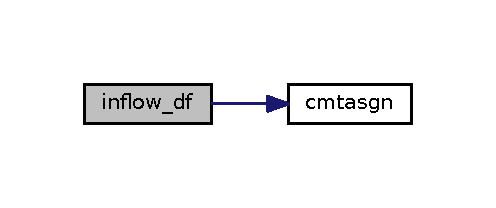
\includegraphics[width=238pt]{group__isurf_ga15e4fb7f0dbe0767ef81c6b291f611cb_cgraph}
\end{center}
\end{figure}


\hypertarget{group__isurf_ga0293ec162f23a55a9e89cf0797cbf2b2}{\index{Inviscid surface terms@{Inviscid surface terms}!outflow\-\_\-df@{outflow\-\_\-df}}
\index{outflow\-\_\-df@{outflow\-\_\-df}!Inviscid surface terms@{Inviscid surface terms}}
\subsubsection[{outflow\-\_\-df}]{\setlength{\rightskip}{0pt plus 5cm}subroutine outflow\-\_\-df (
\begin{DoxyParamCaption}
\item[{integer}]{f, }
\item[{integer}]{e, }
\item[{real, dimension(nvar,lx1$\ast$lz1)}]{wm, }
\item[{real, dimension(nvar,lx1$\ast$lz1)}]{wp, }
\item[{real, dimension(toteq,lx1$\ast$lz1)}]{um, }
\item[{real, dimension(toteq,lx1$\ast$lz1)}]{up, }
\item[{integer}]{nvar}
\end{DoxyParamCaption}
)}}\label{group__isurf_ga0293ec162f23a55a9e89cf0797cbf2b2}


Dolejsi \& Feistauer (2015) Section 8.\-3.\-2.\-2. Very rudimentary ``physical'' boundary conditions. Also encountered in Hartmann \& Houston (2006). A poor default. 


\begin{DoxyParams}{Parameters}
{\em f} & face index from 1 to 2$\ast$ldim\\
\hline
{\em e} & element index\\
\hline
{\em nvar} & number of primitive variables\\
\hline
{\em wm} & primitive variables from flow solution (dimension(nvar,lx1$\ast$lz1),intent(in))\\
\hline
{\em wp} & external dirichlet state's primitive variables (dimension(nvar,lx1$\ast$lz1),intent(out))\\
\hline
{\em um} & conserved variables from flow solution (dimension(toteq,lx1$\ast$lz1),intent(in))\\
\hline
{\em up} & external dirichlet state's conserved variables (dimension(toteq,lx1$\ast$lz1),intent(out)) \\
\hline
\end{DoxyParams}


Here is the call graph for this function\-:\nopagebreak
\begin{figure}[H]
\begin{center}
\leavevmode
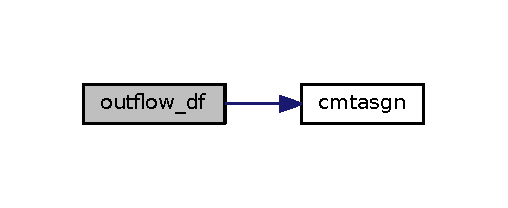
\includegraphics[width=244pt]{group__isurf_ga0293ec162f23a55a9e89cf0797cbf2b2_cgraph}
\end{center}
\end{figure}



\hypertarget{group__vsurf}{\section{Viscous surface terms}
\label{group__vsurf}\index{Viscous surface terms@{Viscous surface terms}}
}
\subsection*{Functions/\-Subroutines}
\begin{DoxyCompactItemize}
\item 
subroutine \hyperlink{group__vsurf_gac863c5b9f5cfae59ded7447a0c5e6d93}{br1auxflux} (e, flux, ujump)
\begin{DoxyCompactList}\small\item\em add B\-R1 auxiliary flux $\frac{1}{2}\left(\mathbf{U}^+-\mathbf{U}^-\right)$ to the gradient for a single element \end{DoxyCompactList}\item 
subroutine \hyperlink{group__vsurf_ga57cdf5eb9ed721fdf3cd454454b47122}{imqqtu} (ummcu, uminus, uplus)
\begin{DoxyCompactList}\small\item\em ummcu = $\mathbf{U}^--\{\{\mathbf{U}\}\}$ \end{DoxyCompactList}\item 
subroutine \hyperlink{group__vsurf_ga98d826061a0ffb225d37cb73b86a9475}{igtu\-\_\-cmt} (qminus, ummcu, hface)
\begin{DoxyCompactList}\small\item\em Computes $G^T U$, the volume integral of $[[u]]\cdot\{\{\nabla v\}\}$, and increments res1 with it. \end{DoxyCompactList}\end{DoxyCompactItemize}


\subsection{Detailed Description}


\subsection{Function/\-Subroutine Documentation}
\hypertarget{group__vsurf_gac863c5b9f5cfae59ded7447a0c5e6d93}{\index{Viscous surface terms@{Viscous surface terms}!br1auxflux@{br1auxflux}}
\index{br1auxflux@{br1auxflux}!Viscous surface terms@{Viscous surface terms}}
\subsubsection[{br1auxflux}]{\setlength{\rightskip}{0pt plus 5cm}subroutine br1auxflux (
\begin{DoxyParamCaption}
\item[{integer}]{e, }
\item[{real, dimension(lx1$\ast$ly1$\ast$lz1,ldim)}]{flux, }
\item[{real, dimension(lx1$\ast$lz1$\ast$2$\ast$ldim,nelt)}]{ujump}
\end{DoxyParamCaption}
)}}\label{group__vsurf_gac863c5b9f5cfae59ded7447a0c5e6d93}


add B\-R1 auxiliary flux $\frac{1}{2}\left(\mathbf{U}^+-\mathbf{U}^-\right)$ to the gradient for a single element 


\begin{DoxyParams}{Parameters}
{\em e} & Indexes the element inside ujump, G\-E\-O\-M and D\-G (intent(in))\\
\hline
{\em ujump} & Jump in a single conserved variable $\left[\left[U\right]\right]$ on all faces of all elements (intent(in))\\
\hline
{\em flux} & On entry\-: gradient $\partial U_i^{-}/\partial x_k$ of a single conserved variable. On exit\-: all three components of auxiliary variable $\mathbf{S}$ of a single conserved variable. (intent(inout)) \\
\hline
\end{DoxyParams}
\hypertarget{group__vsurf_ga98d826061a0ffb225d37cb73b86a9475}{\index{Viscous surface terms@{Viscous surface terms}!igtu\-\_\-cmt@{igtu\-\_\-cmt}}
\index{igtu\-\_\-cmt@{igtu\-\_\-cmt}!Viscous surface terms@{Viscous surface terms}}
\subsubsection[{igtu\-\_\-cmt}]{\setlength{\rightskip}{0pt plus 5cm}subroutine igtu\-\_\-cmt (
\begin{DoxyParamCaption}
\item[{real, dimension(lx1$\ast$lz1,2$\ast$ldim,nelt,$\ast$)}]{qminus, }
\item[{real, dimension(lx1$\ast$lz1$\ast$2$\ast$ldim,nelt,toteq)}]{ummcu, }
\item[{real, dimension(lx1$\ast$lz1$\ast$2$\ast$ldim$\ast$nelt,toteq,3)}]{hface}
\end{DoxyParamCaption}
)}}\label{group__vsurf_ga98d826061a0ffb225d37cb73b86a9475}


Computes $G^T U$, the volume integral of $[[u]]\cdot\{\{\nabla v\}\}$, and increments res1 with it. 


\begin{DoxyParams}{Parameters}
{\em qminus} & qminus contains values of state variables indexed by j$\ast$ at each element's own face points ummcu contains $U-\{\{U\}\}$ \\
\hline
\end{DoxyParams}
Symmetric interior penalty method (S\-I\-P) and Baumann-\/\-Oden have opposite signs for this term. The sign is H\-A\-R\-D\-C\-O\-D\-E\-D here.

gradm1\-\_\-t uses /ctmp1/

Here is the call graph for this function\-:\nopagebreak
\begin{figure}[H]
\begin{center}
\leavevmode
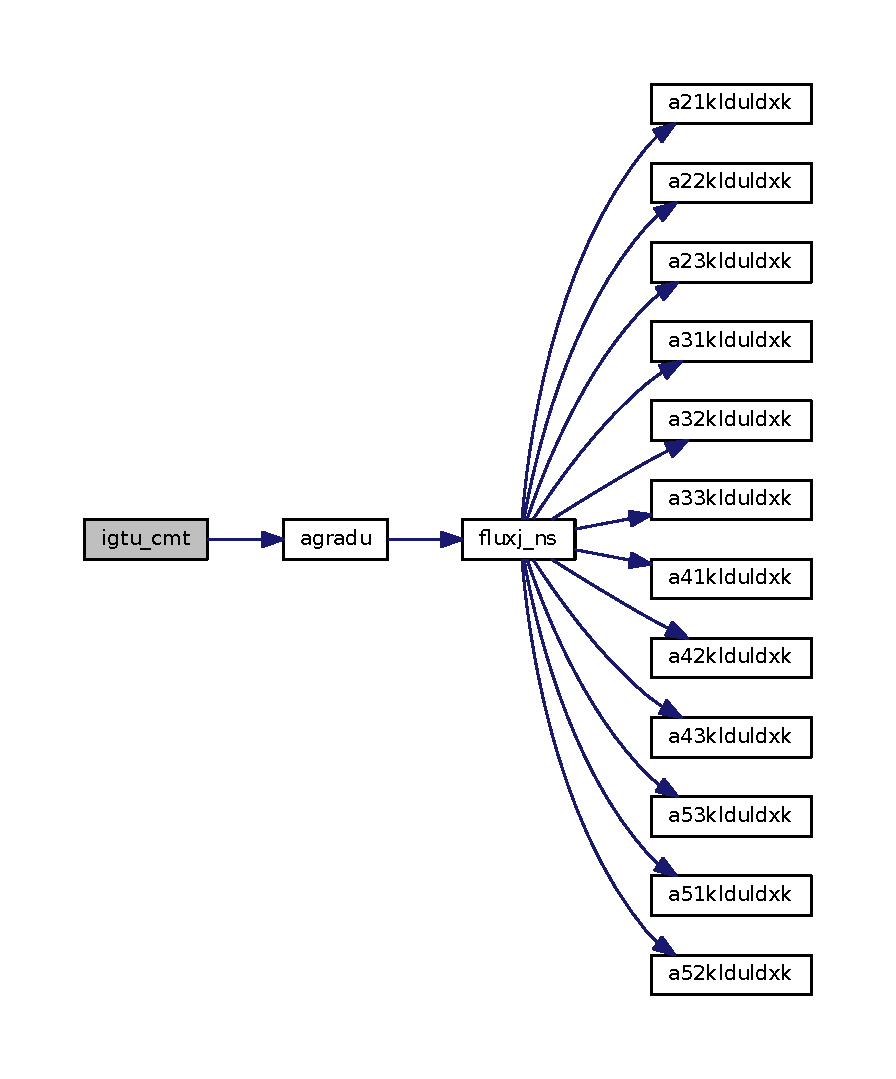
\includegraphics[width=350pt]{group__vsurf_ga98d826061a0ffb225d37cb73b86a9475_cgraph}
\end{center}
\end{figure}


\hypertarget{group__vsurf_ga57cdf5eb9ed721fdf3cd454454b47122}{\index{Viscous surface terms@{Viscous surface terms}!imqqtu@{imqqtu}}
\index{imqqtu@{imqqtu}!Viscous surface terms@{Viscous surface terms}}
\subsubsection[{imqqtu}]{\setlength{\rightskip}{0pt plus 5cm}subroutine imqqtu (
\begin{DoxyParamCaption}
\item[{real, dimension (lx1$\ast$lz1$\ast$2$\ast$ldim$\ast$nelt,toteq)}]{ummcu, }
\item[{real, dimension(lx1$\ast$lz1$\ast$2$\ast$ldim$\ast$nelt,toteq)}]{uminus, }
\item[{real, dimension (lx1$\ast$lz1$\ast$2$\ast$ldim$\ast$nelt,toteq)}]{uplus}
\end{DoxyParamCaption}
)}}\label{group__vsurf_ga57cdf5eb9ed721fdf3cd454454b47122}


ummcu = $\mathbf{U}^--\{\{\mathbf{U}\}\}$ 


\begin{DoxyParams}{Parameters}
{\em ummcu} & ummcu = $\mathbf{U}^--\{\{\mathbf{U}\}\}$ for all faces (intent(out))\\
\hline
{\em uminus} & $\mathbf{U}^-$ for all faces on all elements (intent(in))\\
\hline
{\em uplus} & Neighbor values $\mathbf{U}^+$ for all faces on all elements (intent(in)) \\
\hline
\end{DoxyParams}

\hypertarget{group__flux}{\section{Flux functions and wrappers}
\label{group__flux}\index{Flux functions and wrappers@{Flux functions and wrappers}}
}
\begin{DoxyCompactItemize}
\item 
subroutine \hyperlink{group__flux_ga4498a8903b8de21f2c0afd0d34c5e00c}{sequential\-\_\-flux} (flux, wminus, wplus, uminus, uplus, jaminus, japlus, fluxfunction, nstate, npt)
\begin{DoxyCompactList}\small\item\em Calls two-\/point external fluxfunction $F^{\#}(U^-,U^+)$ at npt points Mostly intended to allow quantity-\/innermost volume flux functions to be used where needed for surface fluxes at boundary points, after $\ast$bc routines provide Dirichlet ``rind'' states in wplus and uplus. \end{DoxyCompactList}\item 
\hypertarget{group__flux_ga07b6f239f6de61d489a639234c55dac3}{subroutine {\bfseries inviscidflux} (wminus, wplus, flux, nstate, nflux)}\label{group__flux_ga07b6f239f6de61d489a639234c55dac3}

\item 
\hypertarget{group__flux_ga799332814e9d69e56ae5cc53dd448ebc}{subroutine {\bfseries surface\-\_\-integral\-\_\-full} (vol, flux)}\label{group__flux_ga799332814e9d69e56ae5cc53dd448ebc}

\item 
\hypertarget{group__flux_ga88fa0428bc395bf4e785ac7c484fc587}{subroutine {\bfseries diffh2graduf} (e, eq, graduf)}\label{group__flux_ga88fa0428bc395bf4e785ac7c484fc587}

\item 
\hypertarget{group__flux_ga41a0b6638f2086e785a2eee46c838140}{subroutine {\bfseries diffh2face} (e, eq, diffhf)}\label{group__flux_ga41a0b6638f2086e785a2eee46c838140}

\item 
\hypertarget{group__flux_ga28b5864db9a8cc5516dff0524e5281dd}{subroutine {\bfseries igu\-\_\-cmt} (flxscr, gdudxk, wminus)}\label{group__flux_ga28b5864db9a8cc5516dff0524e5281dd}

\item 
\hypertarget{group__flux_ga9e1df29c0b6ddab6d384439c68f98361}{subroutine {\bfseries igu\-\_\-dirichlet} (flux, \hyperlink{group__vfjac_ga9087d56c6c467d3ffeb9aa6be3f43e82}{agradu})}\label{group__flux_ga9e1df29c0b6ddab6d384439c68f98361}

\item 
\hypertarget{group__flux_ga549c3560ff566ecc4ebe5a26cd8d7434}{subroutine {\bfseries br1primary} (flux, gdudxk)}\label{group__flux_ga549c3560ff566ecc4ebe5a26cd8d7434}

\item 
\hypertarget{group__flux_gaf5460e23edcfc140cce7884a9e3ebdac}{subroutine {\bfseries agradu\-\_\-normal\-\_\-flux} (flux, graduf)}\label{group__flux_gaf5460e23edcfc140cce7884a9e3ebdac}

\item 
\hypertarget{group__flux_gaf39815444396f97adffa0273bf02d6e5}{subroutine {\bfseries br1bc} (flux)}\label{group__flux_gaf39815444396f97adffa0273bf02d6e5}

\item 
\hypertarget{group__flux_gad4b2470bb6d756ae16a22aa09bff20cd}{subroutine {\bfseries bcflux\-\_\-br1} (flux, f, e)}\label{group__flux_gad4b2470bb6d756ae16a22aa09bff20cd}

\item 
\hypertarget{group__flux_gadcea35e25dbe44ed6a9f9816974a8dc7}{subroutine {\bfseries strong\-\_\-sfc\-\_\-flux} (flux, vflx, e, eq)}\label{group__flux_gadcea35e25dbe44ed6a9f9816974a8dc7}

\item 
\hypertarget{group__flux_ga565a7f26aa4697a900499931ca224e37}{subroutine {\bfseries fluxes\-\_\-full\-\_\-field\-\_\-chold}}\label{group__flux_ga565a7f26aa4697a900499931ca224e37}

\item 
\hypertarget{group__flux_gade9f72409b237ebd1810b9d856f2c0d2}{subroutine {\bfseries fluxes\-\_\-full\-\_\-field\-\_\-old}}\label{group__flux_gade9f72409b237ebd1810b9d856f2c0d2}

\item 
\hypertarget{group__flux_gae3c480e559a6d01be27381e8517a210d}{subroutine {\bfseries inviscidfluxrot} (wminus, wplus, flux, nstate, nflux)}\label{group__flux_gae3c480e559a6d01be27381e8517a210d}

\item 
subroutine \hyperlink{group__flux_gab4541d3a9fc0c10583e47fa4b6cc9f2d}{gtu\-\_\-wrapper} (fatface)
\end{DoxyCompactItemize}


\subsection{Detailed Description}


\subsection{Function/\-Subroutine Documentation}
\hypertarget{group__flux_gab4541d3a9fc0c10583e47fa4b6cc9f2d}{\index{Flux functions and wrappers@{Flux functions and wrappers}!gtu\-\_\-wrapper@{gtu\-\_\-wrapper}}
\index{gtu\-\_\-wrapper@{gtu\-\_\-wrapper}!Flux functions and wrappers@{Flux functions and wrappers}}
\subsubsection[{gtu\-\_\-wrapper}]{\setlength{\rightskip}{0pt plus 5cm}subroutine gtu\-\_\-wrapper (
\begin{DoxyParamCaption}
\item[{real, dimension($\ast$)}]{fatface}
\end{DoxyParamCaption}
)}}\label{group__flux_gab4541d3a9fc0c10583e47fa4b6cc9f2d}
res1+= $\int_{\Gamma} \{\{\mathbf{A}^{\intercal}\nabla v\}\} \cdot \left[\mathbf{U}\right] dA$

res1+= $\int \left(\nabla v\right) \cdot \left(\mathbf{H}^c+\mathbf{H}^d\right)dV$ for each equation (inner), one element at a time (outer) 

Here is the call graph for this function\-:\nopagebreak
\begin{figure}[H]
\begin{center}
\leavevmode
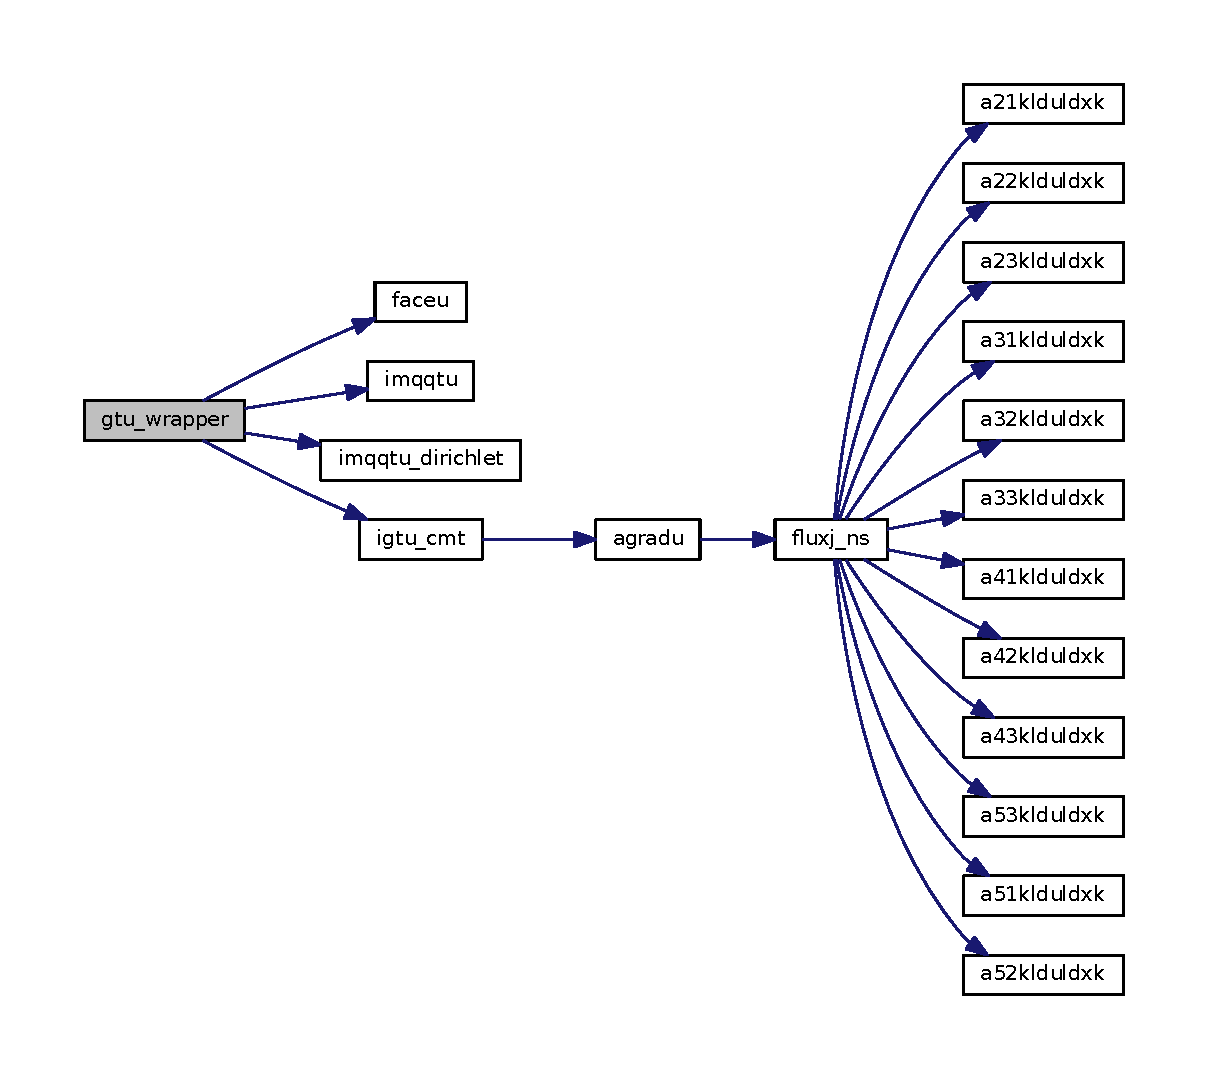
\includegraphics[width=350pt]{group__flux_gab4541d3a9fc0c10583e47fa4b6cc9f2d_cgraph}
\end{center}
\end{figure}


\hypertarget{group__flux_ga4498a8903b8de21f2c0afd0d34c5e00c}{\index{Flux functions and wrappers@{Flux functions and wrappers}!sequential\-\_\-flux@{sequential\-\_\-flux}}
\index{sequential\-\_\-flux@{sequential\-\_\-flux}!Flux functions and wrappers@{Flux functions and wrappers}}
\subsubsection[{sequential\-\_\-flux}]{\setlength{\rightskip}{0pt plus 5cm}subroutine sequential\-\_\-flux (
\begin{DoxyParamCaption}
\item[{real, dimension(toteq,npt)}]{flux, }
\item[{real, dimension(nstate,npt)}]{wminus, }
\item[{real, dimension(nstate,npt)}]{wplus, }
\item[{real, dimension(toteq,npt)}]{uminus, }
\item[{real, dimension(toteq,npt)}]{uplus, }
\item[{real, dimension(3,npt)}]{jaminus, }
\item[{real, dimension(3,npt)}]{japlus, }
\item[{external}]{fluxfunction, }
\item[{}]{nstate, }
\item[{}]{npt}
\end{DoxyParamCaption}
)}}\label{group__flux_ga4498a8903b8de21f2c0afd0d34c5e00c}


Calls two-\/point external fluxfunction $F^{\#}(U^-,U^+)$ at npt points Mostly intended to allow quantity-\/innermost volume flux functions to be used where needed for surface fluxes at boundary points, after $\ast$bc routines provide Dirichlet ``rind'' states in wplus and uplus. 


\begin{DoxyParams}{Parameters}
{\em flux} & Real (intent(out)) $F^{\#}(U^-,U^+)$ on output\\
\hline
{\em wminus} & Real (intent(in)) Primitive variables at one point. Usually $w^-$ at interior nodes\\
\hline
{\em wplus} & Real (intent(in)) Primitive variables at the other point. Usually $w^+$ at rind state or nodes of neighboring element\\
\hline
{\em jaminus} & Real (intent(in)) Mesh metrics at one point.\\
\hline
{\em japlus} & Real (intent(in)) Mesh metrics at the other point.\\
\hline
{\em uminus} & Real (intent(in)) Conserved variables one point. Usually $U^-$ at interior nodes.\\
\hline
{\em uplus} & Real (intent(in)) Conserved variables at the other point. Usually $U^+$ at rind state or nodes of neighboring element \\
\hline
\end{DoxyParams}
External subroutine for $F^{\#}$. See \hyperlink{fluxfn_8f}{fluxfn.\-f} 

Here is the call graph for this function\-:\nopagebreak
\begin{figure}[H]
\begin{center}
\leavevmode
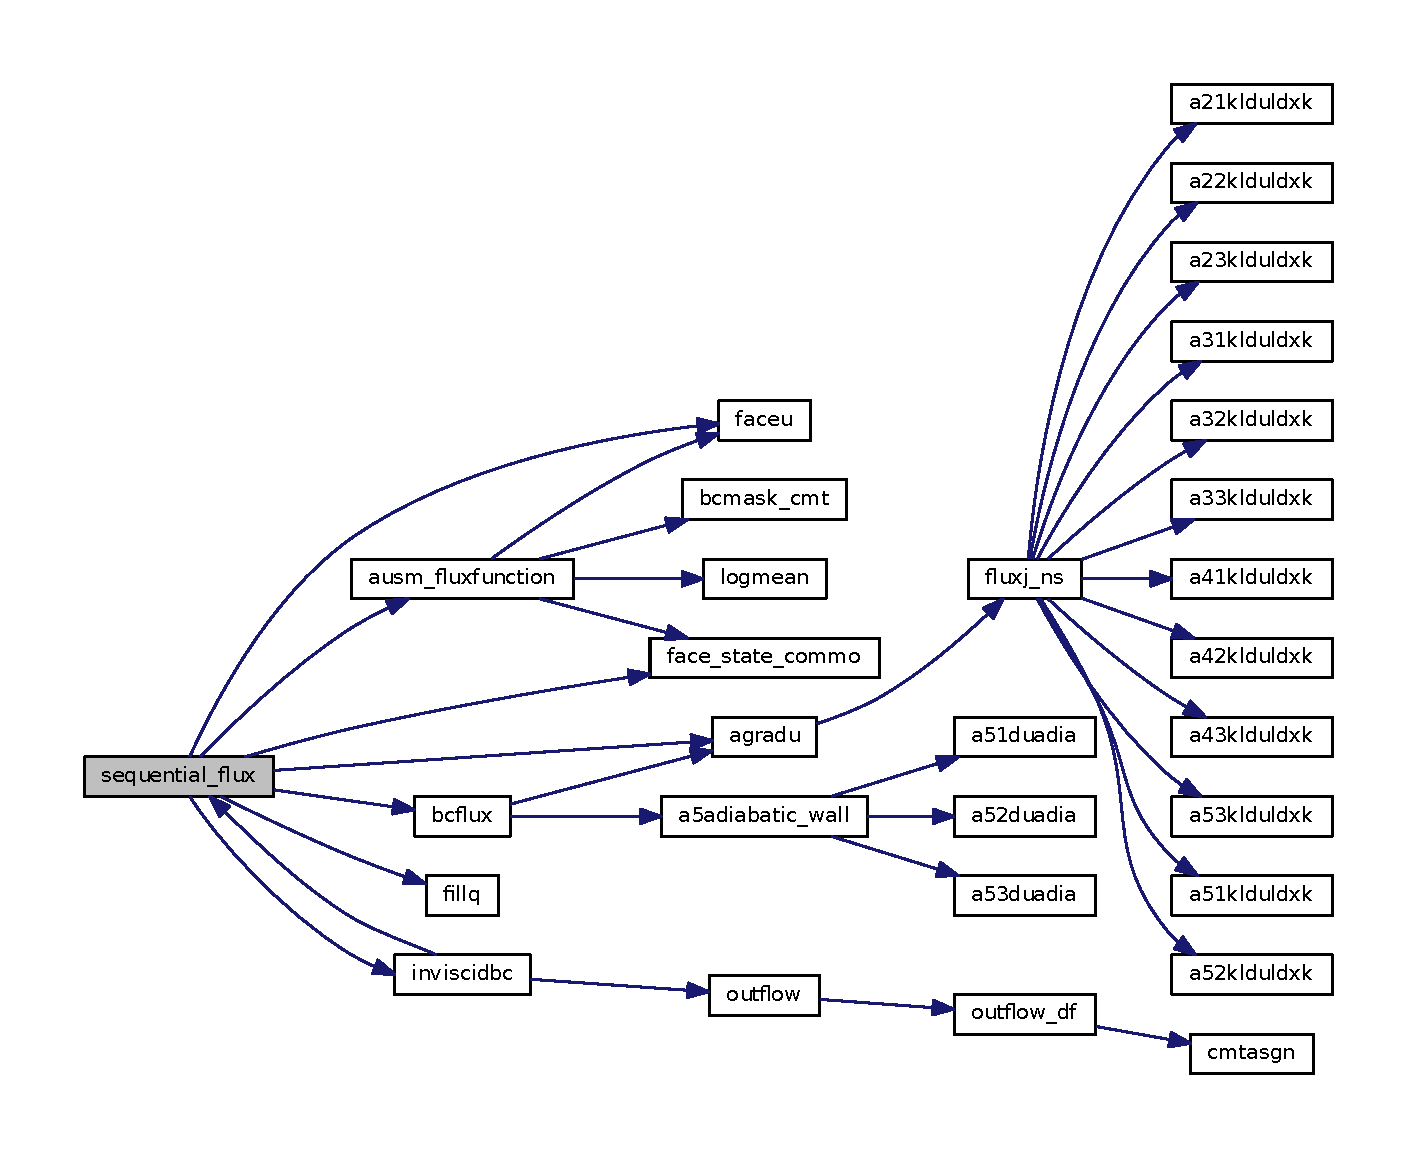
\includegraphics[width=350pt]{group__flux_ga4498a8903b8de21f2c0afd0d34c5e00c_cgraph}
\end{center}
\end{figure}



\hypertarget{group__faceops}{\section{utility functions for manipulating face data}
\label{group__faceops}\index{utility functions for manipulating face data@{utility functions for manipulating face data}}
}

\hypertarget{group__twopoint}{\section{structure for symmetric flux functions in split forms}
\label{group__twopoint}\index{structure for symmetric flux functions in split forms@{structure for symmetric flux functions in split forms}}
}

\hypertarget{group__initialconds}{\section{flow field initialization routines}
\label{group__initialconds}\index{flow field initialization routines@{flow field initialization routines}}
}
\subsection*{Functions/\-Subroutines}
\begin{DoxyCompactItemize}
\item 
\hypertarget{group__initialconds_ga0427858fb7b0c582bcd5ff776de86a09}{subroutine \hyperlink{group__initialconds_ga0427858fb7b0c582bcd5ff776de86a09}{cmtasgn} (ix, iy, iz, e)}\label{group__initialconds_ga0427858fb7b0c582bcd5ff776de86a09}

\begin{DoxyCompactList}\small\item\em Fill /\-N\-E\-K\-U\-S\-E/ and /\-N\-E\-K\-U\-S\-C\-M\-T/ common blocks from a single G\-L\-L node extends nekasgn to C\-M\-T-\/nek without affecting core routines. \end{DoxyCompactList}\item 
subroutine \hyperlink{group__initialconds_ga1be8524b895b1b95b04e8707aa0ba4ae}{cmt\-\_\-ics}
\begin{DoxyCompactList}\small\item\em set initial values of conserved variables in U for C\-M\-T-\/nek \end{DoxyCompactList}\item 
subroutine \hyperlink{group__initialconds_ga3e2114ab9f0c76a032cd4d0f708bdc24}{cmtuic}
\begin{DoxyCompactList}\small\item\em Fresh initialization of conserved variables from useric. \end{DoxyCompactList}\end{DoxyCompactItemize}


\subsection{Detailed Description}


\subsection{Function/\-Subroutine Documentation}
\hypertarget{group__initialconds_ga1be8524b895b1b95b04e8707aa0ba4ae}{\index{flow field initialization routines@{flow field initialization routines}!cmt\-\_\-ics@{cmt\-\_\-ics}}
\index{cmt\-\_\-ics@{cmt\-\_\-ics}!flow field initialization routines@{flow field initialization routines}}
\subsubsection[{cmt\-\_\-ics}]{\setlength{\rightskip}{0pt plus 5cm}subroutine cmt\-\_\-ics (
\begin{DoxyParamCaption}
{}
\end{DoxyParamCaption}
)}}\label{group__initialconds_ga1be8524b895b1b95b04e8707aa0ba4ae}


set initial values of conserved variables in U for C\-M\-T-\/nek 

Over-\/engineered duplicate of setics in core nek5000. Calls cmtuic for a fresh start or my\-\_\-full\-\_\-restart for restart. cmtuic actually initializes the flow field through cmt-\/nek's own dedicated calls to useric. logs min and max of primitive variables as a sanity check in diagnostic I/\-O labeled \char`\"{}\-Cuvwpt,\char`\"{} etc. 

Here is the call graph for this function\-:\nopagebreak
\begin{figure}[H]
\begin{center}
\leavevmode
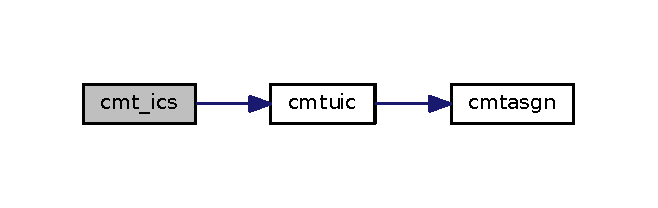
\includegraphics[width=316pt]{group__initialconds_ga1be8524b895b1b95b04e8707aa0ba4ae_cgraph}
\end{center}
\end{figure}


\hypertarget{group__initialconds_ga3e2114ab9f0c76a032cd4d0f708bdc24}{\index{flow field initialization routines@{flow field initialization routines}!cmtuic@{cmtuic}}
\index{cmtuic@{cmtuic}!flow field initialization routines@{flow field initialization routines}}
\subsubsection[{cmtuic}]{\setlength{\rightskip}{0pt plus 5cm}subroutine cmtuic (
\begin{DoxyParamCaption}
{}
\end{DoxyParamCaption}
)}}\label{group__initialconds_ga3e2114ab9f0c76a032cd4d0f708bdc24}


Fresh initialization of conserved variables from useric. 

Calls cmtasgn to interface with userbc, forms conserved variables from scalar primitive variables one grid point at a time, and fills U completely. 

Here is the call graph for this function\-:\nopagebreak
\begin{figure}[H]
\begin{center}
\leavevmode
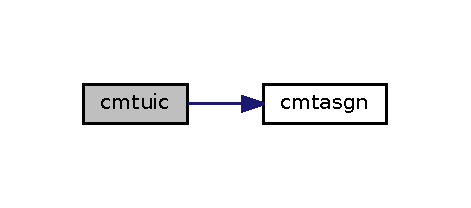
\includegraphics[width=226pt]{group__initialconds_ga3e2114ab9f0c76a032cd4d0f708bdc24_cgraph}
\end{center}
\end{figure}



\hypertarget{group__state}{\section{Thermodynamic state variables from conserved variables}
\label{group__state}\index{Thermodynamic state variables from conserved variables@{Thermodynamic state variables from conserved variables}}
}
\subsection*{Functions/\-Subroutines}
\begin{DoxyCompactItemize}
\item 
subroutine \hyperlink{group__state_ga150496cc6bdf94171d8f6822cd697145}{compute\-\_\-primitive\-\_\-vars} (ilim)
\begin{DoxyCompactList}\small\item\em Compute primitive variables (velocity, thermodynamic state) from conserved unknowns U and store them in S\-O\-L\-N and C\-M\-T\-D\-A\-T\-A. \end{DoxyCompactList}\item 
subroutine \hyperlink{group__state_ga91fd597ad604e7412e8d78a79beefe34}{tdstate} (e, energy)
\begin{DoxyCompactList}\small\item\em calls cmt\-\_\-user\-E\-O\-S in the usr file. Compute thermodynamic state for element e from internal energy and density. \end{DoxyCompactList}\item 
\hypertarget{group__state_ga9e9e837579897a93f40aae1fe6060255}{subroutine \hyperlink{group__state_ga9e9e837579897a93f40aae1fe6060255}{poscheck} (ifail, what)}\label{group__state_ga9e9e837579897a93f40aae1fe6060255}

\begin{DoxyCompactList}\small\item\em if positive posflags, write failure message and exit \end{DoxyCompactList}\end{DoxyCompactItemize}


\subsection{Detailed Description}


\subsection{Function/\-Subroutine Documentation}
\hypertarget{group__state_ga150496cc6bdf94171d8f6822cd697145}{\index{Thermodynamic state variables from conserved variables@{Thermodynamic state variables from conserved variables}!compute\-\_\-primitive\-\_\-vars@{compute\-\_\-primitive\-\_\-vars}}
\index{compute\-\_\-primitive\-\_\-vars@{compute\-\_\-primitive\-\_\-vars}!Thermodynamic state variables from conserved variables@{Thermodynamic state variables from conserved variables}}
\subsubsection[{compute\-\_\-primitive\-\_\-vars}]{\setlength{\rightskip}{0pt plus 5cm}subroutine compute\-\_\-primitive\-\_\-vars (
\begin{DoxyParamCaption}
\item[{integer}]{ilim}
\end{DoxyParamCaption}
)}}\label{group__state_ga150496cc6bdf94171d8f6822cd697145}


Compute primitive variables (velocity, thermodynamic state) from conserved unknowns U and store them in S\-O\-L\-N and C\-M\-T\-D\-A\-T\-A. 


\begin{DoxyParams}{Parameters}
{\em ilim} & ilim is a flag for positivity checks. ilim==0 means {\ttfamily do not perform positivity checks.'' ilim !=0 means}perform positivity checks and exit with a diagnostic dump if density, energy or temperature fall to zero or below at any G\-L\-L node.'' \\
\hline
\end{DoxyParams}
Flags for density, energy and temperature positivity

Density positivity check.

Divide momentum by density to get velocity

Compute kinetic energy using vdot2/3

Compute internal energy. First, subtract volume-\/fraction-\/weighted kinetic energy from total energy.

Then, divide internal energy by density.

Compute density by dividing U1 by gas volume fraction. store in vtrans(\-:,jrho)

Check positivity of internal energy.

Compute thermodynamic state variables cv, T and p. Check temperature positivity using ifailt in /posflags/

call poscheck for each of the posflags and exit if ilim!=0 and any posflag$>$0. Nonzero posflags are set to the global element number where the first positivity failure on each M\-P\-I task was encountered.

Here is the call graph for this function\-:\nopagebreak
\begin{figure}[H]
\begin{center}
\leavevmode
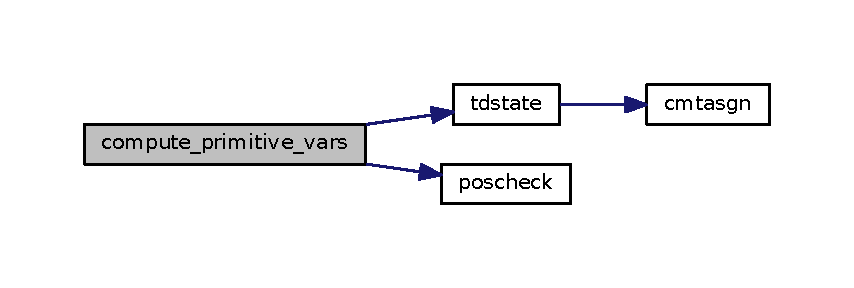
\includegraphics[width=350pt]{group__state_ga150496cc6bdf94171d8f6822cd697145_cgraph}
\end{center}
\end{figure}


\hypertarget{group__state_ga91fd597ad604e7412e8d78a79beefe34}{\index{Thermodynamic state variables from conserved variables@{Thermodynamic state variables from conserved variables}!tdstate@{tdstate}}
\index{tdstate@{tdstate}!Thermodynamic state variables from conserved variables@{Thermodynamic state variables from conserved variables}}
\subsubsection[{tdstate}]{\setlength{\rightskip}{0pt plus 5cm}subroutine tdstate (
\begin{DoxyParamCaption}
\item[{integer}]{e, }
\item[{real, dimension(lx1,ly1,lz1)}]{energy}
\end{DoxyParamCaption}
)}}\label{group__state_ga91fd597ad604e7412e8d78a79beefe34}


calls cmt\-\_\-user\-E\-O\-S in the usr file. Compute thermodynamic state for element e from internal energy and density. 

loop over G\-L\-L nodes in element e. Fill /\-N\-E\-K\-U\-S\-E/ and /nekuscmt/ by nekasgn and cmtasgn calls, respectively.

Compute thermodynamic state from scalars declared in /\-N\-E\-K\-U\-S\-E/ and /nekuscmt/ store state variables in temp,cv,cp,pres and asnd

Check temperature positivity

Fill S\-O\-L\-N and C\-M\-T\-D\-A\-T\-A arrays one G\-L\-L node at a time from scalars in /\-N\-E\-K\-U\-S\-E/ and /nekuscmt/

Here is the call graph for this function\-:\nopagebreak
\begin{figure}[H]
\begin{center}
\leavevmode
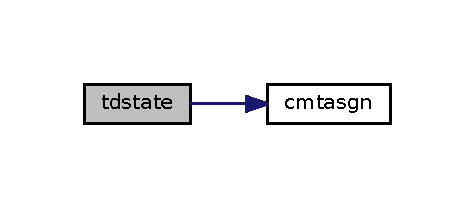
\includegraphics[width=228pt]{group__state_ga91fd597ad604e7412e8d78a79beefe34_cgraph}
\end{center}
\end{figure}



\chapter{File Documentation}
\hypertarget{bc_8f}{\section{bc.\-f File Reference}
\label{bc_8f}\index{bc.\-f@{bc.\-f}}
}


Boundary condition routines.  


\subsection*{Functions/\-Subroutines}
\begin{DoxyCompactItemize}
\item 
\hypertarget{group__bcond_ga45475eec850fc7ef33c51a25b4f86602}{subroutine \hyperlink{group__bcond_ga45475eec850fc7ef33c51a25b4f86602}{inviscidbc} (flux)}\label{group__bcond_ga45475eec850fc7ef33c51a25b4f86602}

\begin{DoxyCompactList}\small\item\em Determining rind state for Dirichlet boundary conditions. \end{DoxyCompactList}\item 
\hypertarget{group__bcond_ga917af547cc29afcf40e2b54c6a97c90d}{subroutine \hyperlink{group__bcond_ga917af547cc29afcf40e2b54c6a97c90d}{bcmask\-\_\-cmt} (bmsk)}\label{group__bcond_ga917af547cc29afcf40e2b54c6a97c90d}

\begin{DoxyCompactList}\small\item\em Mask to make sure Fsharp doesn't clobber boundary faces, where gs\-\_\-op is null This routine intents to take a real array for all face points, bmask, and only zero out faces on boundaries. It is thus not limited to an array only of indicators. \end{DoxyCompactList}\item 
\hypertarget{group__bcond_ga73b8f242bb8ea95b0c7baf512eeac825}{subroutine \hyperlink{group__bcond_ga73b8f242bb8ea95b0c7baf512eeac825}{bcflux} (flux, \hyperlink{group__vfjac_ga9087d56c6c467d3ffeb9aa6be3f43e82}{agradu}, qminus)}\label{group__bcond_ga73b8f242bb8ea95b0c7baf512eeac825}

\begin{DoxyCompactList}\small\item\em Determining I\-G\-U contribution to boundary flux. 0 for artificial viscosity, and strictly interior for physical viscosity. \end{DoxyCompactList}\item 
\hypertarget{group__bcond_ga9a5825c588243a1c261d107376f5a873}{subroutine \hyperlink{group__bcond_ga9a5825c588243a1c261d107376f5a873}{a5adiabatic\-\_\-wall} (eflx, f, e, d\-U, wstate)}\label{group__bcond_ga9a5825c588243a1c261d107376f5a873}

\begin{DoxyCompactList}\small\item\em computes boundary flux for adiabatic wall in igu \end{DoxyCompactList}\item 
subroutine \hyperlink{group__bcond_ga224b6cf6476419f057df67c7a0d05504}{a51duadia} (flux, f, ie, d\-U, wstate)
\begin{DoxyCompactList}\small\item\em same as A51 for volume flux (x-\/direction viscous flux of energy, but \end{DoxyCompactList}\item 
subroutine \hyperlink{group__bcond_gaaaddd14c010da1bce6192846a45b63f2}{a52duadia} (flux, f, ie, d\-U, wstate)
\begin{DoxyCompactList}\small\item\em same as A51 for volume flux (y-\/direction viscous flux of energy, but \end{DoxyCompactList}\item 
subroutine \hyperlink{group__bcond_ga4311cb4d64847bc8b17c653ca9185866}{a53duadia} (flux, f, ie, d\-U, wstate)
\begin{DoxyCompactList}\small\item\em same as A51 for volume flux (z-\/direction viscous flux of energy, but \end{DoxyCompactList}\end{DoxyCompactItemize}


\subsection{Detailed Description}
Boundary condition routines. 
\hypertarget{diffusive__cmt_8f}{\section{diffusive\-\_\-cmt.\-f File Reference}
\label{diffusive__cmt_8f}\index{diffusive\-\_\-cmt.\-f@{diffusive\-\_\-cmt.\-f}}
}


routines for diffusive fluxes. Some surface. Some volume. All pain. Jacobians and other factorizations.  


\subsection*{Functions/\-Subroutines}
\begin{DoxyCompactItemize}
\item 
subroutine \hyperlink{group__vsurf_gac863c5b9f5cfae59ded7447a0c5e6d93}{br1auxflux} (e, flux, ujump)
\begin{DoxyCompactList}\small\item\em add B\-R1 auxiliary flux $\frac{1}{2}\left(\mathbf{U}^+-\mathbf{U}^-\right)$ to the gradient for a single element \end{DoxyCompactList}\item 
subroutine \hyperlink{group__vsurf_ga57cdf5eb9ed721fdf3cd454454b47122}{imqqtu} (ummcu, uminus, uplus)
\begin{DoxyCompactList}\small\item\em ummcu = $\mathbf{U}^--\{\{\mathbf{U}\}\}$ \end{DoxyCompactList}\item 
subroutine \hyperlink{group__bcond_ga01708cdee955465babb7a371d4e5effa}{imqqtu\-\_\-dirichlet} (umubc, wminus, wplus)
\begin{DoxyCompactList}\small\item\em $\left(\mathbf{I}-1/2QQ^T\right)\mathbf{U}\rightarrow\mathbf{U}^--\mathbf{U}^D$ on Dirichlet boundaries. Currently only modifies $\mathbf{U}^+$ in the case of walls. \end{DoxyCompactList}\item 
subroutine \hyperlink{group__vfjac_ga9087d56c6c467d3ffeb9aa6be3f43e82}{agradu} (flux, du, e, eq)
\begin{DoxyCompactList}\small\item\em Transforms the gradients of conserved variables $\nabla \mathbf{U}$ to the viscous flux $\mathbf{H}^{(d)}$ in a single element for a single equation. Particular choice of viscous stress tensor is currently hardcoded for Navier-\/\-Stokes. \end{DoxyCompactList}\item 
subroutine \hyperlink{group__vfjac_ga2c0d85531a9af69b9d464571ca530e5d}{fluxj\-\_\-ns} (flux, gradu, e, eq)
\begin{DoxyCompactList}\small\item\em $ \tau_{ij}=2 \mu\sigma_{ij} + \lambda \Delta \delta_{ij}$ Navier-\/\-Stokes. uservp provides properties stored in S\-O\-L\-N. Implemented via maxima-\/generated code. \end{DoxyCompactList}\item 
\hypertarget{diffusive__cmt_8f_a1c3683ff121ed541c445d78e7d86e85b}{subroutine \hyperlink{diffusive__cmt_8f_a1c3683ff121ed541c445d78e7d86e85b}{fluxj\-\_\-evm} (flux, du, e, eq)}\label{diffusive__cmt_8f_a1c3683ff121ed541c445d78e7d86e85b}

\begin{DoxyCompactList}\small\item\em viscous flux jacobian for entropy viscosity Euler regularization of Guermond and Popov (2014) S\-I\-A\-M J\-A\-M 74(2) that do N\-O\-T overlap with the compressible Navier-\/\-Stokes equations (N\-S). \end{DoxyCompactList}\item 
subroutine \hyperlink{group__diffhvol_ga90ef567419c8aa503af50a7e747c884e}{half\-\_\-iku\-\_\-cmt} (res, diffh, e)
\begin{DoxyCompactList}\small\item\em Compute the integrand $\mathbf{D}^{T}\mathbf{H}^d$ of the weak-\/form volume integral and store it in res1 one element per call. \end{DoxyCompactList}\item 
subroutine \hyperlink{group__vfjac_ga15f8f8f0e3d305dc065f004aa09de57c}{compute\-\_\-transport\-\_\-props}
\begin{DoxyCompactList}\small\item\em Fill vdiff with transport properties. Hardcoded indices for Navier-\/\-Stokes Used for both artificial and physical viscosities. \end{DoxyCompactList}\item 
\hypertarget{group__vfjac_ga34cccfbb67ddce8c68e7f2742a94af96}{subroutine \hyperlink{group__vfjac_ga34cccfbb67ddce8c68e7f2742a94af96}{a51klduldxk} (flux, d\-U, ie)}\label{group__vfjac_ga34cccfbb67ddce8c68e7f2742a94af96}

\begin{DoxyCompactList}\small\item\em W\-R\-I\-T\-E O\-U\-T N\-O\-T\-A\-T\-I\-O\-N. \end{DoxyCompactList}\item 
\hypertarget{group__vfjac_gad8d6f5b90772f9f1082fba425cece421}{subroutine \hyperlink{group__vfjac_gad8d6f5b90772f9f1082fba425cece421}{a52klduldxk} (flux, d\-U, ie)}\label{group__vfjac_gad8d6f5b90772f9f1082fba425cece421}

\begin{DoxyCompactList}\small\item\em W\-R\-I\-T\-E O\-U\-T N\-O\-T\-A\-T\-I\-O\-N. \end{DoxyCompactList}\item 
\hypertarget{group__vfjac_ga68680b2ed51dce76ed38535fee8c7f63}{subroutine \hyperlink{group__vfjac_ga68680b2ed51dce76ed38535fee8c7f63}{a53klduldxk} (flux, d\-U, ie)}\label{group__vfjac_ga68680b2ed51dce76ed38535fee8c7f63}

\begin{DoxyCompactList}\small\item\em W\-R\-I\-T\-E O\-U\-T N\-O\-T\-A\-T\-I\-O\-N. \end{DoxyCompactList}\item 
\hypertarget{group__vfjac_ga7818a3a1981f80b10cfc4f1d93d5babc}{subroutine \hyperlink{group__vfjac_ga7818a3a1981f80b10cfc4f1d93d5babc}{a21klduldxk} (flux, d\-U, ie)}\label{group__vfjac_ga7818a3a1981f80b10cfc4f1d93d5babc}

\begin{DoxyCompactList}\small\item\em W\-R\-I\-T\-E O\-U\-T N\-O\-T\-A\-T\-I\-O\-N. \end{DoxyCompactList}\item 
\hypertarget{group__vfjac_ga608f83273074946557a9015117c11670}{subroutine \hyperlink{group__vfjac_ga608f83273074946557a9015117c11670}{a22klduldxk} (flux, d\-U, ie)}\label{group__vfjac_ga608f83273074946557a9015117c11670}

\begin{DoxyCompactList}\small\item\em W\-R\-I\-T\-E O\-U\-T N\-O\-T\-A\-T\-I\-O\-N. \end{DoxyCompactList}\item 
\hypertarget{group__vfjac_ga9271a9b027c374b2b2fba0f7f0e00a1e}{subroutine \hyperlink{group__vfjac_ga9271a9b027c374b2b2fba0f7f0e00a1e}{a23klduldxk} (flux, d\-U, ie)}\label{group__vfjac_ga9271a9b027c374b2b2fba0f7f0e00a1e}

\begin{DoxyCompactList}\small\item\em W\-R\-I\-T\-E O\-U\-T N\-O\-T\-A\-T\-I\-O\-N. \end{DoxyCompactList}\item 
\hypertarget{group__vfjac_ga3485906a061442ec51929856cc8f4d4a}{subroutine \hyperlink{group__vfjac_ga3485906a061442ec51929856cc8f4d4a}{a31klduldxk} (flux, d\-U, ie)}\label{group__vfjac_ga3485906a061442ec51929856cc8f4d4a}

\begin{DoxyCompactList}\small\item\em W\-R\-I\-T\-E O\-U\-T N\-O\-T\-A\-T\-I\-O\-N. \end{DoxyCompactList}\item 
\hypertarget{group__vfjac_ga2a280e4b1d5fbba00356ca9120709fa0}{subroutine \hyperlink{group__vfjac_ga2a280e4b1d5fbba00356ca9120709fa0}{a32klduldxk} (flux, d\-U, ie)}\label{group__vfjac_ga2a280e4b1d5fbba00356ca9120709fa0}

\begin{DoxyCompactList}\small\item\em W\-R\-I\-T\-E O\-U\-T N\-O\-T\-A\-T\-I\-O\-N. \end{DoxyCompactList}\item 
\hypertarget{group__vfjac_ga4b542714fa89c4288fa5846a11cc28b1}{subroutine \hyperlink{group__vfjac_ga4b542714fa89c4288fa5846a11cc28b1}{a33klduldxk} (flux, d\-U, ie)}\label{group__vfjac_ga4b542714fa89c4288fa5846a11cc28b1}

\begin{DoxyCompactList}\small\item\em W\-R\-I\-T\-E O\-U\-T N\-O\-T\-A\-T\-I\-O\-N. \end{DoxyCompactList}\item 
\hypertarget{group__vfjac_ga8b5ee49aa820086e3596a1a91e9dc799}{subroutine \hyperlink{group__vfjac_ga8b5ee49aa820086e3596a1a91e9dc799}{a41klduldxk} (flux, d\-U, ie)}\label{group__vfjac_ga8b5ee49aa820086e3596a1a91e9dc799}

\begin{DoxyCompactList}\small\item\em W\-R\-I\-T\-E O\-U\-T N\-O\-T\-A\-T\-I\-O\-N. \end{DoxyCompactList}\item 
\hypertarget{group__vfjac_ga7cf0c00202b223c51bed9c61c7937bc6}{subroutine \hyperlink{group__vfjac_ga7cf0c00202b223c51bed9c61c7937bc6}{a42klduldxk} (flux, d\-U, ie)}\label{group__vfjac_ga7cf0c00202b223c51bed9c61c7937bc6}

\begin{DoxyCompactList}\small\item\em W\-R\-I\-T\-E O\-U\-T N\-O\-T\-A\-T\-I\-O\-N. \end{DoxyCompactList}\item 
\hypertarget{group__vfjac_ga7d4c71aaaae94de9cd5f41a93836699a}{subroutine \hyperlink{group__vfjac_ga7d4c71aaaae94de9cd5f41a93836699a}{a43klduldxk} (flux, d\-U, ie)}\label{group__vfjac_ga7d4c71aaaae94de9cd5f41a93836699a}

\begin{DoxyCompactList}\small\item\em W\-R\-I\-T\-E O\-U\-T N\-O\-T\-A\-T\-I\-O\-N. \end{DoxyCompactList}\end{DoxyCompactItemize}


\subsection{Detailed Description}
routines for diffusive fluxes. Some surface. Some volume. All pain. Jacobians and other factorizations. 
\hypertarget{drive1__cmt_8f}{\section{drive1\-\_\-cmt.\-f File Reference}
\label{drive1__cmt_8f}\index{drive1\-\_\-cmt.\-f@{drive1\-\_\-cmt.\-f}}
}


high-\/level driver for C\-M\-T-\/nek  


\subsection*{Functions/\-Subroutines}
\begin{DoxyCompactItemize}
\item 
subroutine \hyperlink{drive1__cmt_8f_af21718debad3a2fefd68afcc5991813a}{cmt\-\_\-nek\-\_\-advance}
\begin{DoxyCompactList}\small\item\em Branch from subroutine nek\-\_\-advance in core/drive1.\-f Advance C\-M\-T-\/nek one time step within nek5000 time loop. \end{DoxyCompactList}\item 
subroutine \hyperlink{drive1__cmt_8f_a001e854c71bfa7c25b504caaa09b7681}{compute\-\_\-rhs\-\_\-and\-\_\-dt}
\begin{DoxyCompactList}\small\item\em Compute right-\/hand-\/side of the semidiscrete conservation law Store it in res1. \end{DoxyCompactList}\item 
\hypertarget{drive1__cmt_8f_a682c25d68683aaedd6aa5c7e7cd166ed}{subroutine \hyperlink{drive1__cmt_8f_a682c25d68683aaedd6aa5c7e7cd166ed}{set\-\_\-tstep\-\_\-coef}}\label{drive1__cmt_8f_a682c25d68683aaedd6aa5c7e7cd166ed}

\begin{DoxyCompactList}\small\item\em Compute coefficients for Runge-\/\-Kutta stages {\bfseries [T\-V\-D\-R\-K]}\}. \end{DoxyCompactList}\item 
\hypertarget{drive1__cmt_8f_a0a2e4794cb7239611d23502b7c312feb}{subroutine \hyperlink{drive1__cmt_8f_a0a2e4794cb7239611d23502b7c312feb}{cmt\-\_\-flow\-\_\-ics}}\label{drive1__cmt_8f_a0a2e4794cb7239611d23502b7c312feb}

\begin{DoxyCompactList}\small\item\em This subroutine must only be called after a restart. It copies arrays that nek5000 reads from S\-L\-N files into their corresponding slots in C\-M\-T\-D\-A\-T\-A. vx stores U(\-:,2,\-:), x-\/momentum. vy stores U(\-:,3,\-:), y-\/momentum. vz stores U(\-:,4,\-:), z-\/momentum. pr stores U(\-:,1,\-:), fluid density The T array stores U(\-:,5,\-:), fluid total energy. \end{DoxyCompactList}\item 
\hypertarget{drive1__cmt_8f_a2d3a6bf3ca463bb62525dd09836d5c43}{subroutine {\bfseries print\-\_\-cmt\-\_\-timers}}\label{drive1__cmt_8f_a2d3a6bf3ca463bb62525dd09836d5c43}

\item 
\hypertarget{drive1__cmt_8f_ad434a1c79e4501bf2b0464edc2636e4b}{subroutine {\bfseries init\-\_\-cmt\-\_\-timers}}\label{drive1__cmt_8f_ad434a1c79e4501bf2b0464edc2636e4b}

\end{DoxyCompactItemize}


\subsection{Detailed Description}
high-\/level driver for C\-M\-T-\/nek 

\subsection{Function/\-Subroutine Documentation}
\hypertarget{drive1__cmt_8f_af21718debad3a2fefd68afcc5991813a}{\index{drive1\-\_\-cmt.\-f@{drive1\-\_\-cmt.\-f}!cmt\-\_\-nek\-\_\-advance@{cmt\-\_\-nek\-\_\-advance}}
\index{cmt\-\_\-nek\-\_\-advance@{cmt\-\_\-nek\-\_\-advance}!drive1_cmt.f@{drive1\-\_\-cmt.\-f}}
\subsubsection[{cmt\-\_\-nek\-\_\-advance}]{\setlength{\rightskip}{0pt plus 5cm}subroutine cmt\-\_\-nek\-\_\-advance (
\begin{DoxyParamCaption}
{}
\end{DoxyParamCaption}
)}}\label{drive1__cmt_8f_af21718debad3a2fefd68afcc5991813a}


Branch from subroutine nek\-\_\-advance in core/drive1.\-f Advance C\-M\-T-\/nek one time step within nek5000 time loop. 

Initialization calls

Runge-\/\-Kutta loop 

Here is the call graph for this function\-:\nopagebreak
\begin{figure}[H]
\begin{center}
\leavevmode
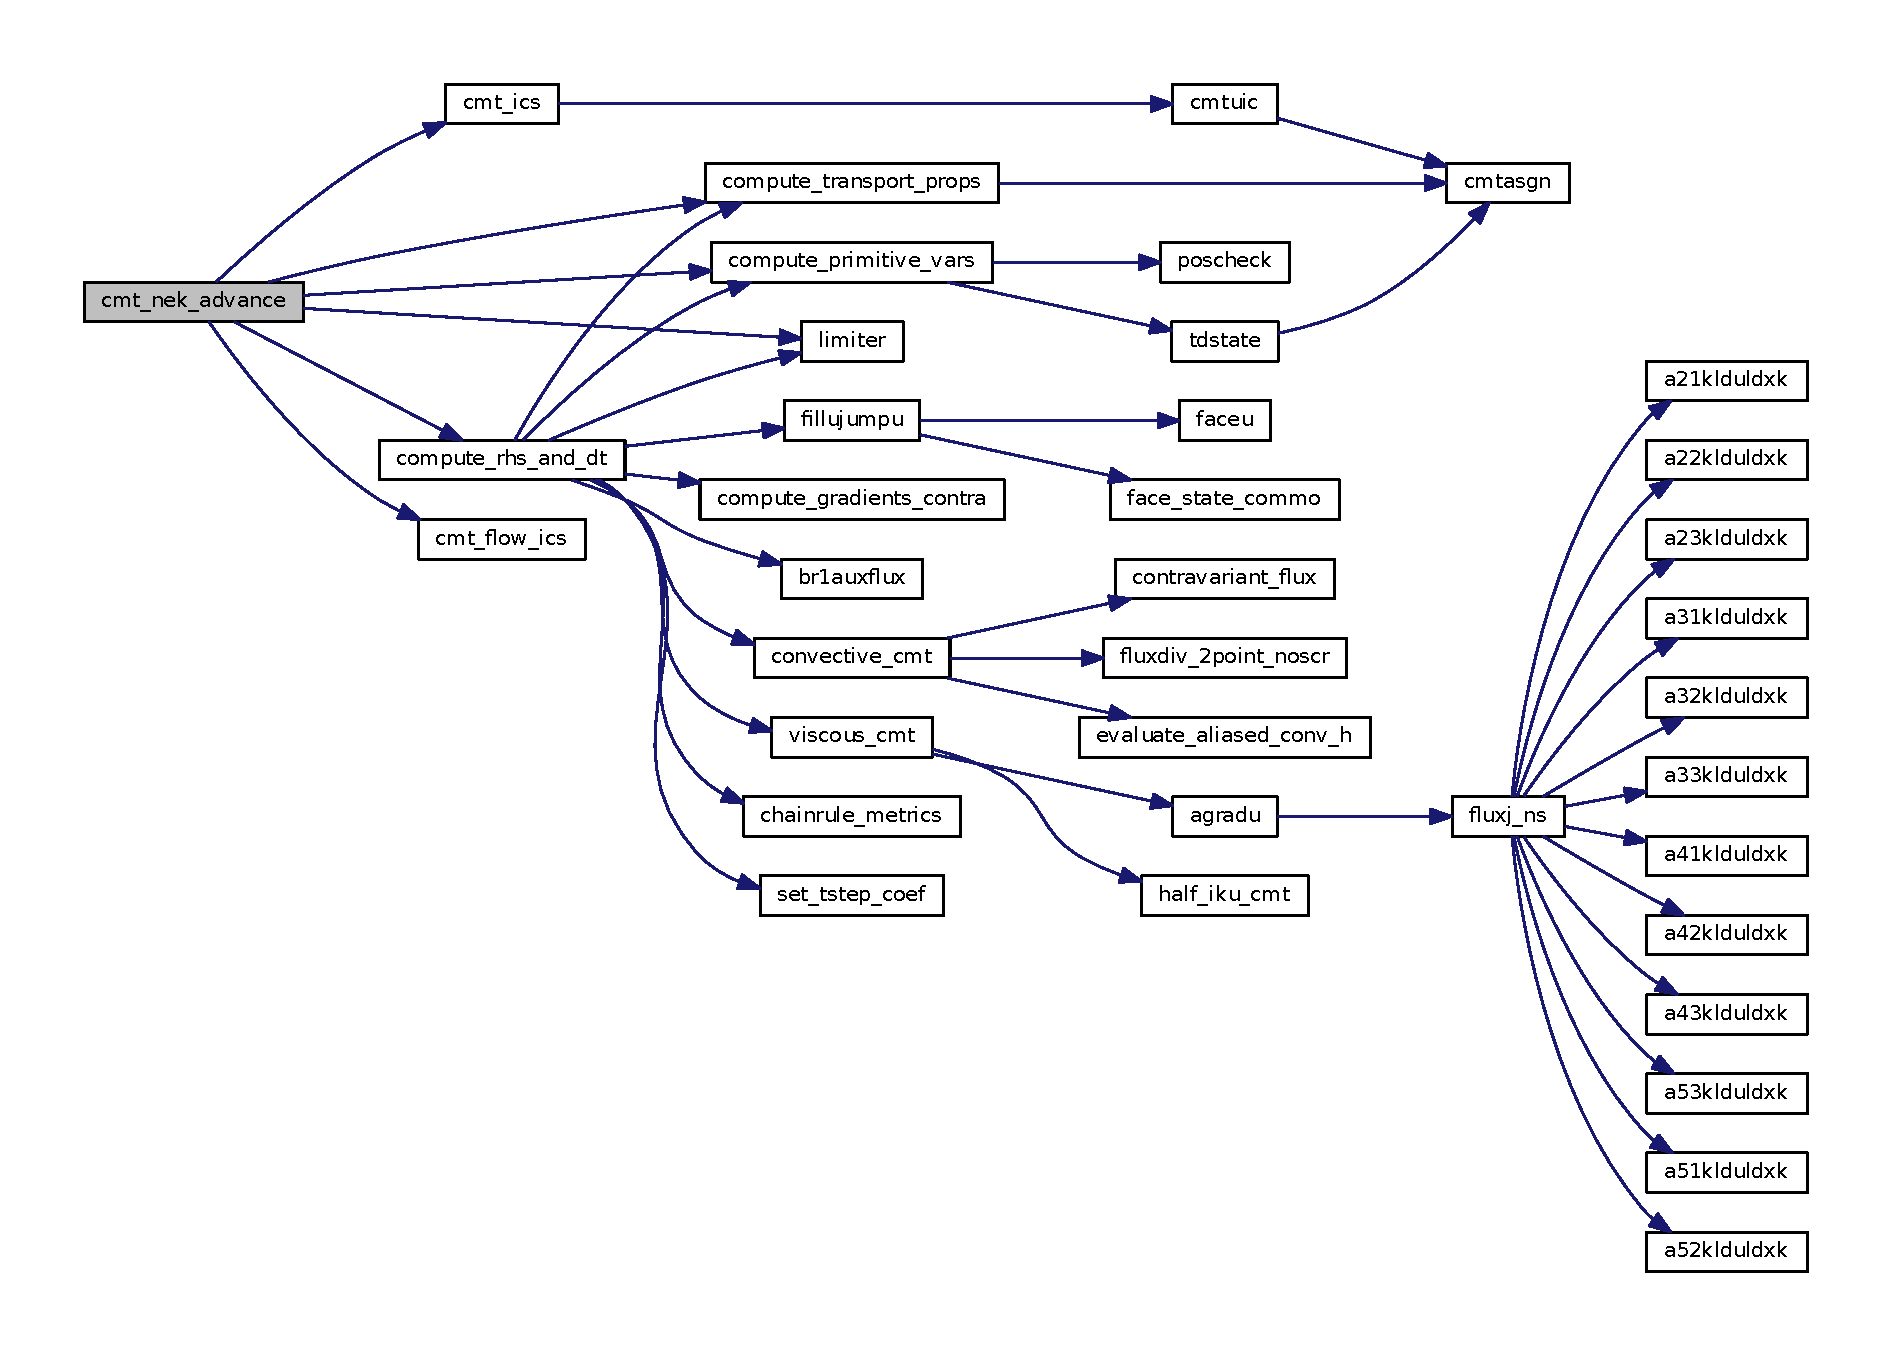
\includegraphics[width=350pt]{drive1__cmt_8f_af21718debad3a2fefd68afcc5991813a_cgraph}
\end{center}
\end{figure}


\hypertarget{drive1__cmt_8f_a001e854c71bfa7c25b504caaa09b7681}{\index{drive1\-\_\-cmt.\-f@{drive1\-\_\-cmt.\-f}!compute\-\_\-rhs\-\_\-and\-\_\-dt@{compute\-\_\-rhs\-\_\-and\-\_\-dt}}
\index{compute\-\_\-rhs\-\_\-and\-\_\-dt@{compute\-\_\-rhs\-\_\-and\-\_\-dt}!drive1_cmt.f@{drive1\-\_\-cmt.\-f}}
\subsubsection[{compute\-\_\-rhs\-\_\-and\-\_\-dt}]{\setlength{\rightskip}{0pt plus 5cm}subroutine compute\-\_\-rhs\-\_\-and\-\_\-dt (
\begin{DoxyParamCaption}
{}
\end{DoxyParamCaption}
)}}\label{drive1__cmt_8f_a001e854c71bfa7c25b504caaa09b7681}


Compute right-\/hand-\/side of the semidiscrete conservation law Store it in res1. 

Restrict via $\mathbf{E}$ to get primitive and conserved variables on interior faces $\mathbf{U}^-$ and neighbor faces $\mathbf{U}^+$; store in C\-M\-T\-S\-U\-R\-F\-L\-X

res1+= $\oint \mathbf{H}^{c\ast}\cdot\mathbf{n}dA$ on face points

res1+= $\int_{\Gamma} \{\{\mathbf{A}\nabla \mathbf{U}\}\} \cdot \left[v\right] dA$ 

Here is the call graph for this function\-:\nopagebreak
\begin{figure}[H]
\begin{center}
\leavevmode
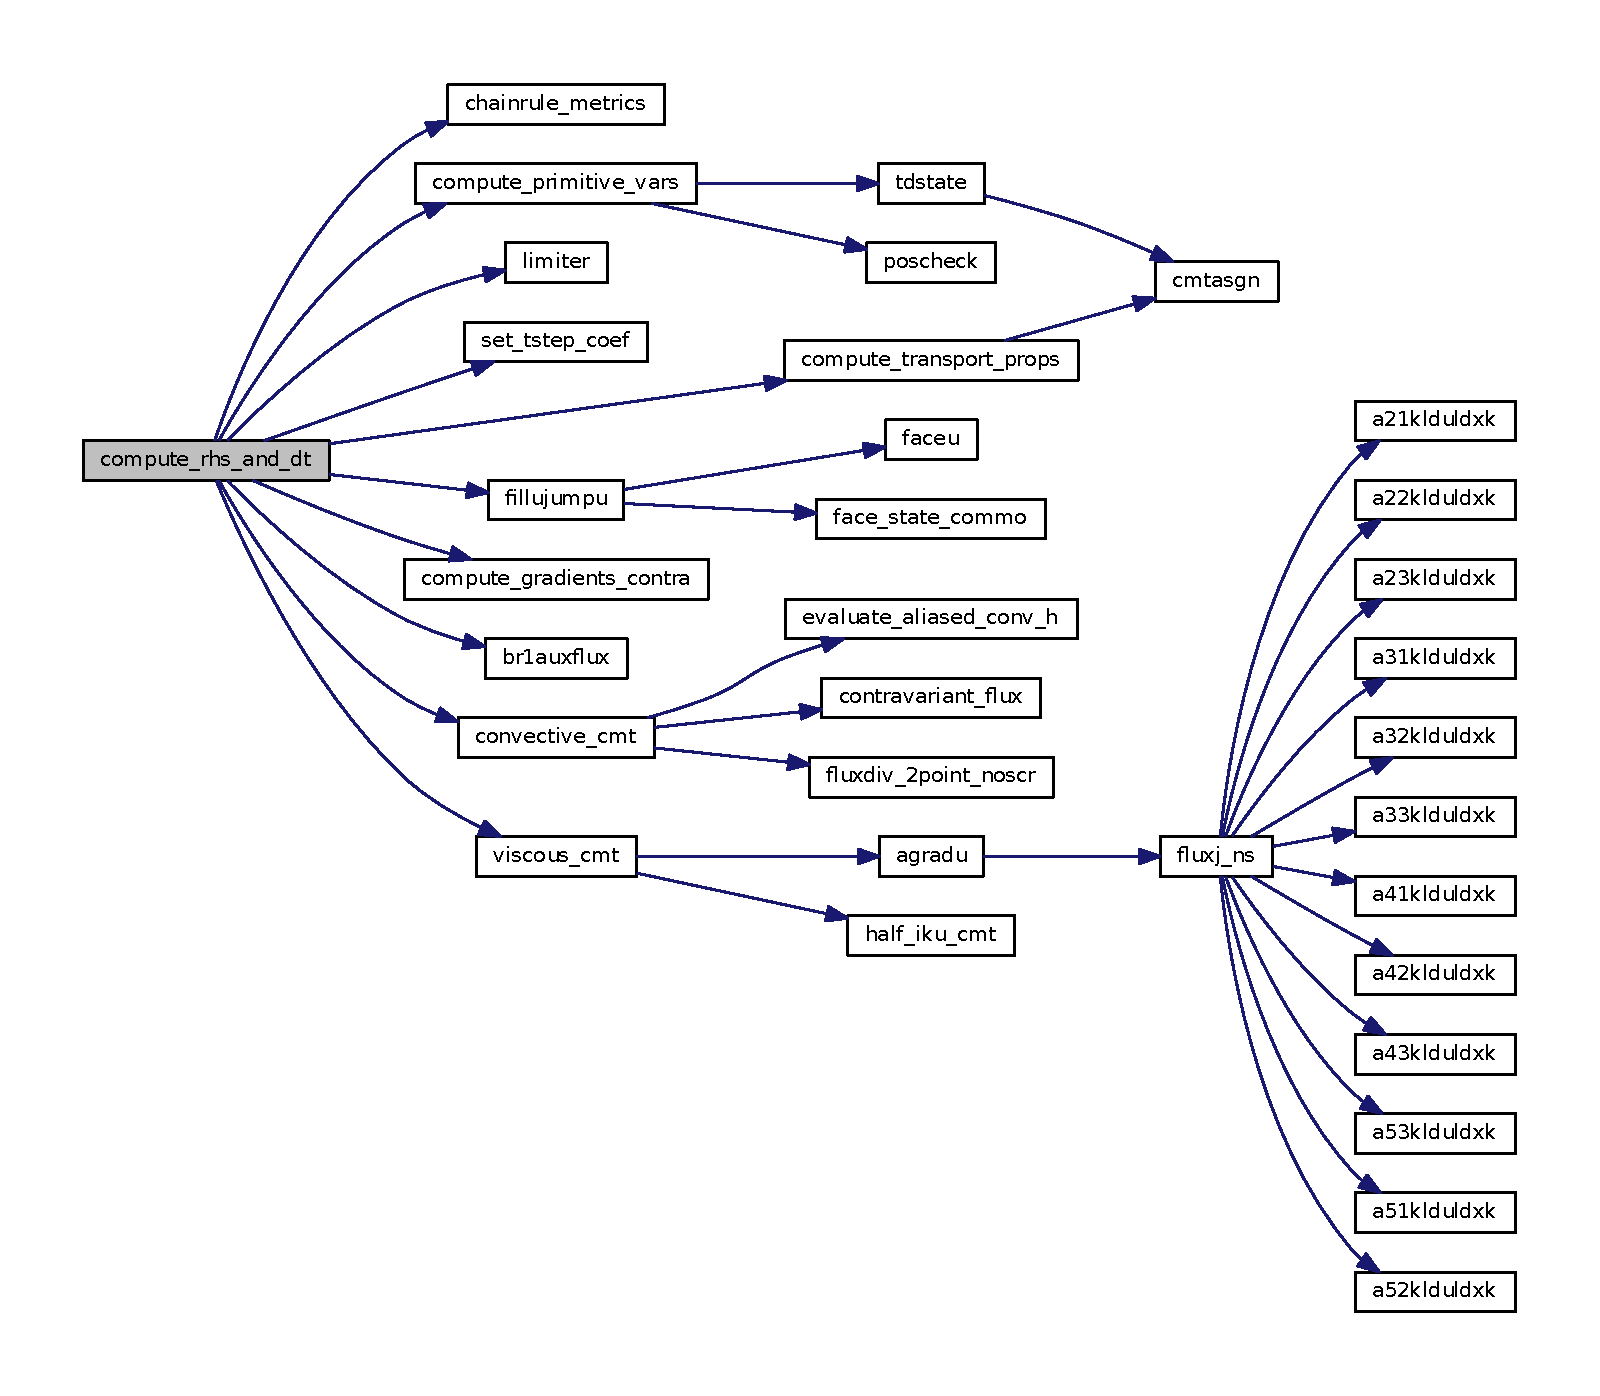
\includegraphics[width=350pt]{drive1__cmt_8f_a001e854c71bfa7c25b504caaa09b7681_cgraph}
\end{center}
\end{figure}



\hypertarget{drive2__cmt_8f}{\section{drive2\-\_\-cmt.\-f File Reference}
\label{drive2__cmt_8f}\index{drive2\-\_\-cmt.\-f@{drive2\-\_\-cmt.\-f}}
}


mid-\/level initialization drivers. Not long for this world.  


\subsection*{Functions/\-Subroutines}
\begin{DoxyCompactItemize}
\item 
\hypertarget{drive2__cmt_8f_a61e619e5f36fba502299223ac6513879}{subroutine \hyperlink{drive2__cmt_8f_a61e619e5f36fba502299223ac6513879}{nek\-\_\-cmt\-\_\-init}}\label{drive2__cmt_8f_a61e619e5f36fba502299223ac6513879}

\begin{DoxyCompactList}\small\item\em This routine was intended to integrate more carefully with nek5000's gs\-\_\-op ifheat was supposed to trigger initialization of Paul Fischer's implementations of D\-G operators K, G and G$^\wedge$\-T, but we never finished keeping up with their work. Right now it's just a wrapper for setup\-\_\-cmt\-\_\-commo. \end{DoxyCompactList}\item 
\hypertarget{drive2__cmt_8f_ae598a12ef00f223232ba04a1e871a924}{subroutine \hyperlink{drive2__cmt_8f_ae598a12ef00f223232ba04a1e871a924}{izero8} (a, n)}\label{drive2__cmt_8f_ae598a12ef00f223232ba04a1e871a924}

\begin{DoxyCompactList}\small\item\em vector routine to zero out kind=8 integers. \end{DoxyCompactList}\item 
\hypertarget{drive2__cmt_8f_a81da0b48bc01bfd806b0a9dfe517578f}{subroutine \hyperlink{drive2__cmt_8f_a81da0b48bc01bfd806b0a9dfe517578f}{limiter}}\label{drive2__cmt_8f_a81da0b48bc01bfd806b0a9dfe517578f}

\begin{DoxyCompactList}\small\item\em positivity-\/preserving limiters. Adjusts conserved variables in U for to ensure that density, pressure and internal energy are positive. Follows Zhang \& Shu (2010) J\-C\-P 229. We did get Lv \& Ihme's (2015) entropy-\/bounded discontinuous Galerkin (E\-B\-D\-G) limiter working, but this is only for perfect gases. \end{DoxyCompactList}\item 
\hypertarget{drive2__cmt_8f_a91f186bf1b4c97f611386abe42e5e547}{real function \hyperlink{drive2__cmt_8f_a91f186bf1b4c97f611386abe42e5e547}{logmean} (l, r)}\label{drive2__cmt_8f_a91f186bf1b4c97f611386abe42e5e547}

\begin{DoxyCompactList}\small\item\em Ismail \& Roe's (2009) version of the logarithmic mean for all possible pairs of values, including equal values. \end{DoxyCompactList}\end{DoxyCompactItemize}


\subsection{Detailed Description}
mid-\/level initialization drivers. Not long for this world. 
\hypertarget{driver3__cmt_8f}{\section{driver3\-\_\-cmt.\-f File Reference}
\label{driver3__cmt_8f}\index{driver3\-\_\-cmt.\-f@{driver3\-\_\-cmt.\-f}}
}


routines for primitive variables, usr-\/file interfaces and properties. Also initializes flow field.  


\subsection*{Functions/\-Subroutines}
\begin{DoxyCompactItemize}
\item 
subroutine \hyperlink{group__state_ga150496cc6bdf94171d8f6822cd697145}{compute\-\_\-primitive\-\_\-vars} (ilim)
\begin{DoxyCompactList}\small\item\em Compute primitive variables (velocity, thermodynamic state) from conserved unknowns U and store them in S\-O\-L\-N and C\-M\-T\-D\-A\-T\-A. \end{DoxyCompactList}\item 
subroutine \hyperlink{group__state_ga91fd597ad604e7412e8d78a79beefe34}{tdstate} (e, energy)
\begin{DoxyCompactList}\small\item\em calls cmt\-\_\-user\-E\-O\-S in the usr file. Compute thermodynamic state for element e from internal energy and density. \end{DoxyCompactList}\item 
\hypertarget{group__initialconds_ga0427858fb7b0c582bcd5ff776de86a09}{subroutine \hyperlink{group__initialconds_ga0427858fb7b0c582bcd5ff776de86a09}{cmtasgn} (ix, iy, iz, e)}\label{group__initialconds_ga0427858fb7b0c582bcd5ff776de86a09}

\begin{DoxyCompactList}\small\item\em Fill /\-N\-E\-K\-U\-S\-E/ and /\-N\-E\-K\-U\-S\-C\-M\-T/ common blocks from a single G\-L\-L node extends nekasgn to C\-M\-T-\/nek without affecting core routines. \end{DoxyCompactList}\item 
subroutine \hyperlink{group__initialconds_ga1be8524b895b1b95b04e8707aa0ba4ae}{cmt\-\_\-ics}
\begin{DoxyCompactList}\small\item\em set initial values of conserved variables in U for C\-M\-T-\/nek \end{DoxyCompactList}\item 
subroutine \hyperlink{group__initialconds_ga3e2114ab9f0c76a032cd4d0f708bdc24}{cmtuic}
\begin{DoxyCompactList}\small\item\em Fresh initialization of conserved variables from useric. \end{DoxyCompactList}\item 
\hypertarget{group__state_ga9e9e837579897a93f40aae1fe6060255}{subroutine \hyperlink{group__state_ga9e9e837579897a93f40aae1fe6060255}{poscheck} (ifail, what)}\label{group__state_ga9e9e837579897a93f40aae1fe6060255}

\begin{DoxyCompactList}\small\item\em if positive posflags, write failure message and exit \end{DoxyCompactList}\end{DoxyCompactItemize}


\subsection{Detailed Description}
routines for primitive variables, usr-\/file interfaces and properties. Also initializes flow field. 
\hypertarget{eqnsolver__cmt_8f}{\section{eqnsolver\-\_\-cmt.\-f File Reference}
\label{eqnsolver__cmt_8f}\index{eqnsolver\-\_\-cmt.\-f@{eqnsolver\-\_\-cmt.\-f}}
}


Routines for entire terms on R\-H\-S. Mostly volume integrals.  


\subsection*{Functions/\-Subroutines}
\begin{DoxyCompactItemize}
\item 
subroutine \hyperlink{group__diffhvol_ga6d611a250fb98acf77e8a3880c0e608d}{viscous\-\_\-cmt} (e, eq)
\begin{DoxyCompactList}\small\item\em Volume integral for diffusive terms. \end{DoxyCompactList}\item 
subroutine \hyperlink{group__vsurf_ga98d826061a0ffb225d37cb73b86a9475}{igtu\-\_\-cmt} (qminus, ummcu, hface)
\begin{DoxyCompactList}\small\item\em Computes $G^T U$, the volume integral of $[[u]]\cdot\{\{\nabla v\}\}$, and increments res1 with it. \end{DoxyCompactList}\item 
subroutine \hyperlink{group__convhvol_ga77e7d7a46950fcbbf072e8e900cee272}{convective\-\_\-cmt} (e)
\begin{DoxyCompactList}\small\item\em Evaluates inviscid volume terms for all toteq equations in two-\/point split form (Equation~\ref{shortvol} and adds them to res1(\-:,\-:,\-:,e,\-:). \end{DoxyCompactList}\item 
\hypertarget{eqnsolver__cmt_8f_a2135bd9a2e75728f817f2b8af7124073}{subroutine {\bfseries fluxdiv\-\_\-2point\-\_\-slow} (res, e, ja)}\label{eqnsolver__cmt_8f_a2135bd9a2e75728f817f2b8af7124073}

\item 
\hypertarget{eqnsolver__cmt_8f_aff3fe4ef3d2532483001e44143232058}{subroutine {\bfseries fluxdiv\-\_\-2point\-\_\-scr} (res, fcons, e, ja)}\label{eqnsolver__cmt_8f_aff3fe4ef3d2532483001e44143232058}

\item 
subroutine \hyperlink{group__convhvol_ga72c1cbe51bc537e14ec8927e62f0e3f3}{fluxdiv\-\_\-2point\-\_\-noscr} (res, fcons, e, ja)
\begin{DoxyCompactList}\small\item\em Evaluates the two-\/point split form (Equations~\ref{splitr} through \ref{splitt}) of the volume integral $\int v \nabla\cdot\mathbf{H}^c dV$ and the discontinuous surface flux $\oint v \mathbf{H}^c\cdot\mathbf{n} dA$ for the inviscid flux function in a single element. \end{DoxyCompactList}\item 
subroutine \hyperlink{group__convhvol_gab4831bb28a78e1c8fd3ec09854bd15ad}{fluxdiv\-\_\-strong\-\_\-contra} (e)
\begin{DoxyCompactList}\small\item\em Computes $\int v \nabla\cdot\mathbf{H}^c dV$ in aliased strong form for element $e$, and increments res1 with it. \end{DoxyCompactList}\item 
subroutine \hyperlink{group__convhvol_gad9d70d83f1184d25495812d637698102}{evaluate\-\_\-aliased\-\_\-conv\-\_\-h} (e)
\begin{DoxyCompactList}\small\item\em Evaluates consistent (i.\-e. $F^{\#}(U_{i,j,k},U_{l,j,k})=H_{(eq),i},i=l$) flux function at all G\-L\-L nodes and stores it in convh. \end{DoxyCompactList}\item 
\hypertarget{group__convhvol_ga89ba8fe53f8afc523597773aca62a270}{subroutine \hyperlink{group__convhvol_ga89ba8fe53f8afc523597773aca62a270}{fluxdiv\-\_\-dealiased\-\_\-weak\-\_\-chain} (e)}\label{group__convhvol_ga89ba8fe53f8afc523597773aca62a270}

\begin{DoxyCompactList}\small\item\em $(\nabla v)\cdot \mathbf{H}^c=\mathcal{I}^{\intercal}\mathbf{D}^{\intercal}\cdots$ for equation eq, element e \end{DoxyCompactList}\item 
\hypertarget{eqnsolver__cmt_8f_a67c37779e77c6d9a630d38fe92314c23}{subroutine {\bfseries fluxdiv\-\_\-weak\-\_\-chain} (e)}\label{eqnsolver__cmt_8f_a67c37779e77c6d9a630d38fe92314c23}

\item 
subroutine \hyperlink{group__convhvol_ga72103225babeca7679ef8b9a41d08f2e}{contravariant\-\_\-flux} (frst, fxyz, ja, nel)
\begin{DoxyCompactList}\small\item\em Transforms consistent (i.\-e. $F^{\#}(U_{i,j,k},U_{l,j,k})=H_{(eq),i},i=l$) flux for one conserved variable to the contravariant frame by contracting H\-\_\-i with J diag $\left(\partial r_j/\partial x_i\right)$. \end{DoxyCompactList}\item 
\hypertarget{eqnsolver__cmt_8f_a16ab9195e1b629e65603f74643f877bb}{subroutine {\bfseries compute\-\_\-forcing} (e, eq\-\_\-num)}\label{eqnsolver__cmt_8f_a16ab9195e1b629e65603f74643f877bb}

\item 
\hypertarget{eqnsolver__cmt_8f_aa10e48ce3eda6377da8f35c3287fc72c}{subroutine {\bfseries cmtusrf} (e)}\label{eqnsolver__cmt_8f_aa10e48ce3eda6377da8f35c3287fc72c}

\end{DoxyCompactItemize}


\subsection{Detailed Description}
Routines for entire terms on R\-H\-S. Mostly volume integrals. 

\hypertarget{face_8f}{\section{face.\-f File Reference}
\label{face_8f}\index{face.\-f@{face.\-f}}
}


low-\/level initialization drivers. Eventually to be superceded by nek5000 core D\-G handles and operators.  


\subsection*{Functions/\-Subroutines}
\begin{DoxyCompactItemize}
\item 
\hypertarget{face_8f_a8efaf08cb6f5e3f2d453dc8195fdedc3}{subroutine {\bfseries iface\-\_\-vert\-\_\-int8cmt} (nx, ny, nz, fa, va, jz0, jz1, nel)}\label{face_8f_a8efaf08cb6f5e3f2d453dc8195fdedc3}

\item 
\hypertarget{face_8f_ac6a7aef7d985d0dbcfccfca53c4c7fc2}{subroutine {\bfseries setup\-\_\-cmt\-\_\-gs} (dg\-\_\-hndl, nx, ny, nz, nel, melg, vertex, gnv, gnf)}\label{face_8f_ac6a7aef7d985d0dbcfccfca53c4c7fc2}

\item 
\hypertarget{face_8f_a7030c76781d497bc17d369a40670ef59}{subroutine {\bfseries setup\-\_\-cmt\-\_\-commo}}\label{face_8f_a7030c76781d497bc17d369a40670ef59}

\item 
\hypertarget{face_8f_ab10a3afa8911c08464a660346cad3c5a}{subroutine {\bfseries cmt\-\_\-set\-\_\-fc\-\_\-ptr} (nel, nx, ny, nz, nface, iface)}\label{face_8f_ab10a3afa8911c08464a660346cad3c5a}

\item 
\hypertarget{face_8f_a250af663ab54c8e8777f671b93c6c4ac}{subroutine {\bfseries full2face\-\_\-cmt} (nel, nx, ny, nz, iface, faces, vols)}\label{face_8f_a250af663ab54c8e8777f671b93c6c4ac}

\item 
\hypertarget{face_8f_a8837dacbadf0fe4f899f2768bb606deb}{subroutine {\bfseries add\-\_\-face2full\-\_\-cmt} (nel, nx, ny, nz, iface, vols, faces)}\label{face_8f_a8837dacbadf0fe4f899f2768bb606deb}

\end{DoxyCompactItemize}


\subsection{Detailed Description}
low-\/level initialization drivers. Eventually to be superceded by nek5000 core D\-G handles and operators. 
\hypertarget{fluxfn_8f}{\section{fluxfn.\-f File Reference}
\label{fluxfn_8f}\index{fluxfn.\-f@{fluxfn.\-f}}
}


Riemann solvers, other rocflu miscellany and two-\/point fluxes.  


\subsection*{Functions/\-Subroutines}
\begin{DoxyCompactItemize}
\item 
\hypertarget{fluxfn_8f_aa0303cef4d920383bd1c82425e0ca07d}{subroutine {\bfseries kgrotfluxfunction} (ntot, nm, rl, ul, vl, wl, pl, al, tl, rr, ur, vr, wr, pr, ar, tr, flx, el, er)}\label{fluxfn_8f_aa0303cef4d920383bd1c82425e0ca07d}

\item 
\hypertarget{group__isurf_ga2b8162e02f3f2266c59f717fa1363226}{subroutine \hyperlink{group__isurf_ga2b8162e02f3f2266c59f717fa1363226}{ausm\-\_\-fluxfunction} (ntot, nx, ny, nz, nm, fs, rl, ul, vl, wl, pl, al, tl, rr, ur, vr, wr, pr, ar, tr, flx, el, er)}\label{group__isurf_ga2b8162e02f3f2266c59f717fa1363226}

\begin{DoxyCompactList}\small\item\em Computes inviscid numerical surface flux from A\-U\-S\-M+ Riemann solver. \end{DoxyCompactList}\item 
\hypertarget{fluxfn_8f_a3a083fcb64cd04500931d07c3c271a3d}{subroutine {\bfseries centralinviscid\-\_\-fluxfunction} (ntot, nx, ny, nz, fs, ul, pl, ur, pr, flx)}\label{fluxfn_8f_a3a083fcb64cd04500931d07c3c271a3d}

\item 
\hypertarget{fluxfn_8f_acbc3512b880f3599497696d179efcaf4}{subroutine {\bfseries llf\-\_\-euler} (flx, ul, ur, wl, wr, nrm, dum)}\label{fluxfn_8f_acbc3512b880f3599497696d179efcaf4}

\item 
\hypertarget{fluxfn_8f_aa210cc6f937700f2161b8ef80941b1b7}{subroutine {\bfseries llf\-\_\-euler\-\_\-vec} (wminus, uplus, flux, nstate)}\label{fluxfn_8f_aa210cc6f937700f2161b8ef80941b1b7}

\item 
\hypertarget{fluxfn_8f_acdcfc163b5cd7fad3949be97707176d0}{subroutine {\bfseries kennedygruber} (flx, ul, ur, wl, wr, jal, jar)}\label{fluxfn_8f_acdcfc163b5cd7fad3949be97707176d0}

\item 
\hypertarget{fluxfn_8f_a59e9fe9c53edce67292dbcb47f7c3853}{subroutine {\bfseries kepec\-\_\-ch} (flx, ul, ur, wl, wr, jal, jar)}\label{fluxfn_8f_a59e9fe9c53edce67292dbcb47f7c3853}

\item 
\hypertarget{fluxfn_8f_a25cb36e6b50d76a9d6d788b9c3656808}{subroutine {\bfseries kennedygruber\-\_\-vec} (z, flux, nstate, nflux)}\label{fluxfn_8f_a25cb36e6b50d76a9d6d788b9c3656808}

\item 
\hypertarget{fluxfn_8f_abf0b8321ecdfdf41f3a2259935c250c9}{subroutine {\bfseries trivial}}\label{fluxfn_8f_abf0b8321ecdfdf41f3a2259935c250c9}

\item 
\hypertarget{fluxfn_8f_a3263d754d306110417d51b61cc67a28b}{subroutine {\bfseries rhoe\-\_\-to\-\_\-e} (fatface, nf, ns)}\label{fluxfn_8f_a3263d754d306110417d51b61cc67a28b}

\item 
\hypertarget{fluxfn_8f_a3264aa63a47559ee42fcf884419d86ca}{subroutine {\bfseries parameter\-\_\-vector\-\_\-vol} (z, zt, ut, e, idum)}\label{fluxfn_8f_a3264aa63a47559ee42fcf884419d86ca}

\item 
\hypertarget{fluxfn_8f_ac2c150a9f3b7c48db9387a5d1840ee5d}{subroutine {\bfseries kepec\-\_\-duplicated} (wminus, wplus, flux)}\label{fluxfn_8f_ac2c150a9f3b7c48db9387a5d1840ee5d}

\end{DoxyCompactItemize}


\subsection{Detailed Description}
Riemann solvers, other rocflu miscellany and two-\/point fluxes. 
\hypertarget{intpdiff_8f}{\section{intpdiff.\-f File Reference}
\label{intpdiff_8f}\index{intpdiff.\-f@{intpdiff.\-f}}
}


interpolation and differentiation routines not already provided by nek5000  


\subsection*{Functions/\-Subroutines}
\begin{DoxyCompactItemize}
\item 
subroutine \hyperlink{intpdiff_8f_a5320a5bf1c50695504168747afc66c93}{compute\-\_\-gradients} (e)
\begin{DoxyCompactList}\small\item\em Compute gradients of conserved variables (W\-I\-T\-H\-O\-U\-T volume fraction weighting) for a single element. Store them in gradu in /\-C\-M\-T\-G\-R\-A\-D\-U/. Uses legacy chain-\/rule metrics in D\-X\-Y\-Z (rxm1, etc.) and N\-O\-T freestream-\/preserving metrics. \end{DoxyCompactList}\item 
subroutine \hyperlink{intpdiff_8f_a65689efbb78eee023a3a9a7d4b9caff7}{set\-\_\-dealias\-\_\-face}
\begin{DoxyCompactList}\small\item\em Fills arrays in /\-F\-A\-C\-E\-W\-Z/ with Gauss-\/\-Legendre quadrature weights on the fine grid for dealiasing surface integrals. \end{DoxyCompactList}\item 
\hypertarget{intpdiff_8f_a08d6fc46ac6dac9935c672df973519c9}{subroutine \hyperlink{intpdiff_8f_a08d6fc46ac6dac9935c672df973519c9}{cmt\-\_\-metrics} (istp)}\label{intpdiff_8f_a08d6fc46ac6dac9935c672df973519c9}

\begin{DoxyCompactList}\small\item\em compute freestream-\/preserving metrics $Ja^i$ for transforming fluxes $F$ to $\tilde{F}$ in a contravariant frame according to Kopriva (2006) Follows methodology in F\-L\-U\-X\-O (github.\-com/project-\/fluxo/fluxo.git) Basically, isoparametric mappings are not freestream preserving. D\-G\-S\-E\-M needs metrics computed from low-\/order geometry interpolated up to polynomial order (when lx1$>$ngeo) O\-R ``dealiased'' metrics (when ngeo$>$lx1) \end{DoxyCompactList}\item 
\hypertarget{intpdiff_8f_a354b767c6b8ae014e7292c05e45157c6}{subroutine {\bfseries xyztriv} (xl, yl, zl, nxl, nyl, nzl, e)}\label{intpdiff_8f_a354b767c6b8ae014e7292c05e45157c6}

\item 
\hypertarget{intpdiff_8f_adbe1ea1506fd5b21cfd8cab10fe0dbc1}{subroutine {\bfseries get\-\_\-int\-\_\-gll2gll} (ip, mx, md)}\label{intpdiff_8f_adbe1ea1506fd5b21cfd8cab10fe0dbc1}

\item 
\hypertarget{intpdiff_8f_a5d574fca7f7d37eff7a8d4403234b933}{subroutine {\bfseries gen\-\_\-int\-\_\-gll2gll} (jgl, jgt, mp, np, w)}\label{intpdiff_8f_a5d574fca7f7d37eff7a8d4403234b933}

\item 
\hypertarget{intpdiff_8f_a6f38dc1f5c137244ae1e261f5bd8279d}{subroutine {\bfseries proj\-\_\-legmodal} (promat, nin, nout)}\label{intpdiff_8f_a6f38dc1f5c137244ae1e261f5bd8279d}

\item 
\hypertarget{intpdiff_8f_acf24494d8b1303f196d15df7ee49f3ec}{subroutine {\bfseries discard\-\_\-rows} (trunc, matrix, nsmall, nlarge)}\label{intpdiff_8f_acf24494d8b1303f196d15df7ee49f3ec}

\item 
\hypertarget{intpdiff_8f_a2fb7b91baaeb2779459b988214efeb9e}{subroutine {\bfseries vandermonde\-\_\-legendre} (v, z, nx)}\label{intpdiff_8f_a2fb7b91baaeb2779459b988214efeb9e}

\item 
\hypertarget{intpdiff_8f_a8f6017ff4e0e2f0d51ed4e1ab69b4f4d}{subroutine {\bfseries gradm11\-\_\-t} (grad, uxyz, csgn, e)}\label{intpdiff_8f_a8f6017ff4e0e2f0d51ed4e1ab69b4f4d}

\item 
\hypertarget{intpdiff_8f_ad76b847e0448d4a237eca9f4f316ebac}{subroutine {\bfseries gradm11\-\_\-t\-\_\-contra} (grad, uxyz, csgn, e)}\label{intpdiff_8f_ad76b847e0448d4a237eca9f4f316ebac}

\item 
\hypertarget{intpdiff_8f_a0d378518f250568824942e9d861a008e}{subroutine {\bfseries gradm1\-\_\-t} (u, ux, uy, uz)}\label{intpdiff_8f_a0d378518f250568824942e9d861a008e}

\end{DoxyCompactItemize}
{\bf }\par
\begin{DoxyCompactItemize}
\item 
subroutine \hyperlink{intpdiff_8f_a4bc9678542951a32332a86f8baf88f23}{compute\-\_\-gradients\-\_\-contra} (e)
\begin{DoxyCompactList}\small\item\em Compute gradients of conserved variables (W\-I\-T\-H\-O\-U\-T volume fraction weighting) for a single element. Store them in gradu in /\-C\-M\-T\-G\-R\-A\-D\-U/. Uses freestream-\/preserving metrics that cmt\-\_\-metrics computes and stores in rx. \end{DoxyCompactList}\end{DoxyCompactItemize}

{\bf }\par
\begin{DoxyCompactItemize}
\item 
\hypertarget{intpdiff_8f_a996a690b6a44c187b06422d8f039344c}{subroutine \hyperlink{intpdiff_8f_a996a690b6a44c187b06422d8f039344c}{chainrule\-\_\-metrics} (istp)}\label{intpdiff_8f_a996a690b6a44c187b06422d8f039344c}

\begin{DoxyCompactList}\small\item\em Keep chain-\/rule metrics as a stop-\/gap until cmt\-\_\-metrics works on deformed elements. Also fills jface with jacobian of mesh on mesh faces, w2m1 with quadrature weights, and dstrong with derivative matrix and appropriate weights for strong-\/form surface integrals. \end{DoxyCompactList}\end{DoxyCompactItemize}



\subsection{Detailed Description}
interpolation and differentiation routines not already provided by nek5000 

\subsection{Function/\-Subroutine Documentation}
\hypertarget{intpdiff_8f_a5320a5bf1c50695504168747afc66c93}{\index{intpdiff.\-f@{intpdiff.\-f}!compute\-\_\-gradients@{compute\-\_\-gradients}}
\index{compute\-\_\-gradients@{compute\-\_\-gradients}!intpdiff.f@{intpdiff.\-f}}
\subsubsection[{compute\-\_\-gradients}]{\setlength{\rightskip}{0pt plus 5cm}subroutine compute\-\_\-gradients (
\begin{DoxyParamCaption}
\item[{integer}]{e}
\end{DoxyParamCaption}
)}}\label{intpdiff_8f_a5320a5bf1c50695504168747afc66c93}


Compute gradients of conserved variables (W\-I\-T\-H\-O\-U\-T volume fraction weighting) for a single element. Store them in gradu in /\-C\-M\-T\-G\-R\-A\-D\-U/. Uses legacy chain-\/rule metrics in D\-X\-Y\-Z (rxm1, etc.) and N\-O\-T freestream-\/preserving metrics. 


\begin{DoxyParams}{Parameters}
{\em e} & e is intent(in). It is the index for the current element in the element loop in compute\-\_\-rhs\-\_\-and\-\_\-dt \\
\hline
\end{DoxyParams}
Divide conserved variables by volume fraction

Differentiate in the reference element. local\-\_\-grad routines are in core/navier5.\-f

Convert d/dr to d/dx via chain-\/rule metrics.\hypertarget{intpdiff_8f_a4bc9678542951a32332a86f8baf88f23}{\index{intpdiff.\-f@{intpdiff.\-f}!compute\-\_\-gradients\-\_\-contra@{compute\-\_\-gradients\-\_\-contra}}
\index{compute\-\_\-gradients\-\_\-contra@{compute\-\_\-gradients\-\_\-contra}!intpdiff.f@{intpdiff.\-f}}
\subsubsection[{compute\-\_\-gradients\-\_\-contra}]{\setlength{\rightskip}{0pt plus 5cm}subroutine compute\-\_\-gradients\-\_\-contra (
\begin{DoxyParamCaption}
\item[{integer}]{e}
\end{DoxyParamCaption}
)}}\label{intpdiff_8f_a4bc9678542951a32332a86f8baf88f23}


Compute gradients of conserved variables (W\-I\-T\-H\-O\-U\-T volume fraction weighting) for a single element. Store them in gradu in /\-C\-M\-T\-G\-R\-A\-D\-U/. Uses freestream-\/preserving metrics that cmt\-\_\-metrics computes and stores in rx. 


\begin{DoxyParams}{Parameters}
{\em e} & e is intent(in). It is the index for the current element in the element loop in compute\-\_\-rhs\-\_\-and\-\_\-dt \\
\hline
\end{DoxyParams}
Divide conserved variables by volume fraction

Differentiate conserved variables in the reference element. local\-\_\-grad routines are in core/navier5.\-f \hypertarget{intpdiff_8f_a65689efbb78eee023a3a9a7d4b9caff7}{\index{intpdiff.\-f@{intpdiff.\-f}!set\-\_\-dealias\-\_\-face@{set\-\_\-dealias\-\_\-face}}
\index{set\-\_\-dealias\-\_\-face@{set\-\_\-dealias\-\_\-face}!intpdiff.f@{intpdiff.\-f}}
\subsubsection[{set\-\_\-dealias\-\_\-face}]{\setlength{\rightskip}{0pt plus 5cm}subroutine set\-\_\-dealias\-\_\-face (
\begin{DoxyParamCaption}
{}
\end{DoxyParamCaption}
)}}\label{intpdiff_8f_a65689efbb78eee023a3a9a7d4b9caff7}


Fills arrays in /\-F\-A\-C\-E\-W\-Z/ with Gauss-\/\-Legendre quadrature weights on the fine grid for dealiasing surface integrals. 

Gauss-\/\-Legendre quadrature weights. Z\-W\-G\-L lives in core/speclib.\-f

Tensor product in two dimensions for a face of a 3\-D element.

faces are just edges in 1\-D. No tensor product
\hypertarget{outflow__bc_8f}{\section{outflow\-\_\-bc.\-f File Reference}
\label{outflow__bc_8f}\index{outflow\-\_\-bc.\-f@{outflow\-\_\-bc.\-f}}
}


Dirichlet states for outflow boundary conditions wrapper for other B\-C routines. Just one for now. More to come.  


\subsection*{Functions/\-Subroutines}
\begin{DoxyCompactItemize}
\item 
subroutine \hyperlink{outflow__bc_8f_ac197c7083c48cd1062073f9c2b56b573}{outflow} (f, e, wminus, wplus, uminus, uplus, nvar)
\item 
subroutine \hyperlink{group__isurf_ga0293ec162f23a55a9e89cf0797cbf2b2}{outflow\-\_\-df} (f, e, wm, wp, um, up, nvar)
\begin{DoxyCompactList}\small\item\em Dolejsi \& Feistauer (2015) Section 8.\-3.\-2.\-2. Very rudimentary ``physical'' boundary conditions. Also encountered in Hartmann \& Houston (2006). A poor default. \end{DoxyCompactList}\item 
\hypertarget{outflow__bc_8f_a97fe193b365ccda49446db3dab8bf08d}{subroutine {\bfseries outflow\-\_\-rflu} (nvar, f, e, facew, wbc)}\label{outflow__bc_8f_a97fe193b365ccda49446db3dab8bf08d}

\item 
\hypertarget{outflow__bc_8f_a52d692beffa8873b023900968d713a1c}{subroutine {\bfseries bcondoutflowperf} (bc\-Opt, pout, sxn, syn, szn, cpgas, mol, rho, rhou, rhov, rhow, rhoe, press, rhob, rhoub, rhovb, rhowb, rhoeb)}\label{outflow__bc_8f_a52d692beffa8873b023900968d713a1c}

\end{DoxyCompactItemize}


\subsection{Detailed Description}
Dirichlet states for outflow boundary conditions wrapper for other B\-C routines. Just one for now. More to come. 

\subsection{Function/\-Subroutine Documentation}
\hypertarget{outflow__bc_8f_ac197c7083c48cd1062073f9c2b56b573}{\index{outflow\-\_\-bc.\-f@{outflow\-\_\-bc.\-f}!outflow@{outflow}}
\index{outflow@{outflow}!outflow_bc.f@{outflow\-\_\-bc.\-f}}
\subsubsection[{outflow}]{\setlength{\rightskip}{0pt plus 5cm}subroutine outflow (
\begin{DoxyParamCaption}
\item[{integer}]{f, }
\item[{integer}]{e, }
\item[{real, dimension(nvar,lx1$\ast$lz1)}]{wminus, }
\item[{real, dimension(nvar,lx1$\ast$lz1)}]{wplus, }
\item[{real, dimension(toteq,lx1$\ast$lz1)}]{uminus, }
\item[{real, dimension(toteq,lx1$\ast$lz1)}]{uplus, }
\item[{integer}]{nvar}
\end{DoxyParamCaption}
)}}\label{outflow__bc_8f_ac197c7083c48cd1062073f9c2b56b573}

\begin{DoxyParams}{Parameters}
{\em f} & face index from 1 to 2$\ast$ldim\\
\hline
{\em e} & element index\\
\hline
{\em nvar} & number of primitive variables\\
\hline
{\em wminus} & primitive variables from flow solution (dimension(nvar,lx1$\ast$lz1),intent(in))\\
\hline
{\em wplus} & external dirichlet state's primitive variables (dimension(nvar,lx1$\ast$lz1),intent(out))\\
\hline
{\em uminus} & conserved variables from flow solution (dimension(toteq,lx1$\ast$lz1),intent(in))\\
\hline
{\em uplus} & external dirichlet state's conserved variables (dimension(toteq,lx1$\ast$lz1),intent(out)) \\
\hline
\end{DoxyParams}


Here is the call graph for this function\-:\nopagebreak
\begin{figure}[H]
\begin{center}
\leavevmode
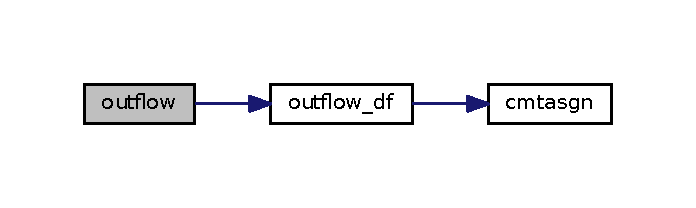
\includegraphics[width=334pt]{outflow__bc_8f_ac197c7083c48cd1062073f9c2b56b573_cgraph}
\end{center}
\end{figure}



\hypertarget{step_8f}{\section{step.\-f File Reference}
\label{step_8f}\index{step.\-f@{step.\-f}}
}


time stepping and mesh spacing routines  


\subsection*{Functions/\-Subroutines}
\begin{DoxyCompactItemize}
\item 
\hypertarget{step_8f_aef8ae89f8ba871aeeec3e23341ffb99d}{subroutine {\bfseries setdtcmt}}\label{step_8f_aef8ae89f8ba871aeeec3e23341ffb99d}

\item 
\hypertarget{step_8f_ac6c3e476ccf64918db5879cc3078847d}{subroutine {\bfseries mindr} (mdr, diffno)}\label{step_8f_ac6c3e476ccf64918db5879cc3078847d}

\item 
\hypertarget{step_8f_a7b5ee2daf5c645627c0bfa9d89591d54}{real function {\bfseries dist2} (x1, y1, x2, y2)}\label{step_8f_a7b5ee2daf5c645627c0bfa9d89591d54}

\item 
\hypertarget{step_8f_a8b53ec0abcf4891f6ed2580c004e1260}{subroutine {\bfseries compute\-\_\-grid\-\_\-h} (h, x, y, z)}\label{step_8f_a8b53ec0abcf4891f6ed2580c004e1260}

\item 
\hypertarget{step_8f_acf204694af344054555925065ba3e7e5}{subroutine {\bfseries glinvcol2max} (col2m, a, b, n, s)}\label{step_8f_acf204694af344054555925065ba3e7e5}

\item 
\hypertarget{step_8f_a1036e181fb73dc698c2bebd20e1d205b}{subroutine {\bfseries glsqinvcolmin} (col2m, a, b, n, s)}\label{step_8f_a1036e181fb73dc698c2bebd20e1d205b}

\item 
\hypertarget{step_8f_a1c6f5326ef92206ed5db09f28221eec1}{subroutine {\bfseries compute\-\_\-mesh\-\_\-h} (h, x, y, z)}\label{step_8f_a1c6f5326ef92206ed5db09f28221eec1}

\end{DoxyCompactItemize}


\subsection{Detailed Description}
time stepping and mesh spacing routines 
\hypertarget{surface__fluxes_8f}{\section{surface\-\_\-fluxes.\-f File Reference}
\label{surface__fluxes_8f}\index{surface\-\_\-fluxes.\-f@{surface\-\_\-fluxes.\-f}}
}


Routines for surface terms on R\-H\-S.  


\subsection*{Functions/\-Subroutines}
\begin{DoxyCompactItemize}
\item 
\hypertarget{group__isurf_gaecf15d43e4c71d130e4ef9e4a6a7821a}{subroutine \hyperlink{group__isurf_gaecf15d43e4c71d130e4ef9e4a6a7821a}{fillujumpu}}\label{group__isurf_gaecf15d43e4c71d130e4ef9e4a6a7821a}

\begin{DoxyCompactList}\small\item\em overwrite beginning of /\-C\-M\-T\-S\-U\-R\-F\-L\-X/ with $-[[\mathbf{U}]]$ for flux of auxiliary variable in the viscous flux of Bassi and Rebay computed in br1auxflux. \end{DoxyCompactList}\item 
subroutine \hyperlink{group__isurf_ga0013a607a259d0c07734b1816f8c9f60}{fluxes\-\_\-full\-\_\-field\-\_\-kg}
\begin{DoxyCompactList}\small\item\em Restrict and copy face data and compute inviscid numerical flux $\oint \mathbf{H}^{c\ast}\cdot\mathbf{n}dA$ on face points. This particular wrapper is for the symmetric flux of Kennedy and Gruber. \end{DoxyCompactList}\item 
subroutine \hyperlink{group__isurf_ga272adf58402c1bfb170c8667bf6be790}{faceu} (ivar, yourface)
\begin{DoxyCompactList}\small\item\em Restrict and copy face data for conserved variables $U_{\mbox{ivar}}$. Wraps full2face\-\_\-cmt for each element; a single call to full2face with $U$ will not work because element varies with the outermost index of the u array. \end{DoxyCompactList}\item 
subroutine \hyperlink{group__isurf_gae375bb9d6acee4eff74aa072206109a2}{fillq} (jvar, field, wminus, yourface)
\begin{DoxyCompactList}\small\item\em Restrict and copy face data for one full field and store it in index jvar in wminus. \end{DoxyCompactList}\item 
subroutine \hyperlink{group__isurf_ga317b9a948c8717ad9c64e0fae72c8641}{dg\-\_\-face\-\_\-avg} (mine, nf, nstate, handle)
\begin{DoxyCompactList}\small\item\em Overwrite values stored at points on faces with the average with its values in the neighboring face without duplication. Replaces $mine$ with $\{\{mine\}\}$. \end{DoxyCompactList}\item 
subroutine \hyperlink{group__isurf_ga53412d5d95cd62ca86dd08374a330b02}{face\-\_\-state\-\_\-commo} (mine, yours, nf, nstate, handle)
\begin{DoxyCompactList}\small\item\em Sends face values $v^-$ stored in ``mine'' to the neighbor that shares that face and copies the neighbor's values $v^+$ at each face into ``yours.''. \end{DoxyCompactList}\item 
subroutine \hyperlink{group__isurf_gaf55d5b18c1b922832898c46176f13386}{avg\-\_\-and\-\_\-jump} (avg, jump, scratch, nf, nstate, handle)
\begin{DoxyCompactList}\small\item\em Overwrites $w^-$ at interior face points stored in avg with $\{\{w\}\}$. jump gets filled with $[[w]]$. \end{DoxyCompactList}\item 
\hypertarget{surface__fluxes_8f_aeaa6969f01eddd2eae8367f610d54d8b}{subroutine {\bfseries face\-\_\-flux\-\_\-commo} (flux1, flux2, nf, neq, handle)}\label{surface__fluxes_8f_aeaa6969f01eddd2eae8367f610d54d8b}

\end{DoxyCompactItemize}
{\bf }\par
\begin{DoxyCompactItemize}
\item 
subroutine \hyperlink{group__flux_ga4498a8903b8de21f2c0afd0d34c5e00c}{sequential\-\_\-flux} (flux, wminus, wplus, uminus, uplus, jaminus, japlus, fluxfunction, nstate, npt)
\begin{DoxyCompactList}\small\item\em Calls two-\/point external fluxfunction $F^{\#}(U^-,U^+)$ at npt points Mostly intended to allow quantity-\/innermost volume flux functions to be used where needed for surface fluxes at boundary points, after $\ast$bc routines provide Dirichlet ``rind'' states in wplus and uplus. \end{DoxyCompactList}\item 
\hypertarget{group__flux_ga07b6f239f6de61d489a639234c55dac3}{subroutine {\bfseries inviscidflux} (wminus, wplus, flux, nstate, nflux)}\label{group__flux_ga07b6f239f6de61d489a639234c55dac3}

\item 
\hypertarget{group__flux_ga799332814e9d69e56ae5cc53dd448ebc}{subroutine {\bfseries surface\-\_\-integral\-\_\-full} (vol, flux)}\label{group__flux_ga799332814e9d69e56ae5cc53dd448ebc}

\item 
\hypertarget{group__flux_ga88fa0428bc395bf4e785ac7c484fc587}{subroutine {\bfseries diffh2graduf} (e, eq, graduf)}\label{group__flux_ga88fa0428bc395bf4e785ac7c484fc587}

\item 
\hypertarget{group__flux_ga41a0b6638f2086e785a2eee46c838140}{subroutine {\bfseries diffh2face} (e, eq, diffhf)}\label{group__flux_ga41a0b6638f2086e785a2eee46c838140}

\item 
\hypertarget{group__flux_ga28b5864db9a8cc5516dff0524e5281dd}{subroutine {\bfseries igu\-\_\-cmt} (flxscr, gdudxk, wminus)}\label{group__flux_ga28b5864db9a8cc5516dff0524e5281dd}

\item 
\hypertarget{group__flux_ga9e1df29c0b6ddab6d384439c68f98361}{subroutine {\bfseries igu\-\_\-dirichlet} (flux, \hyperlink{group__vfjac_ga9087d56c6c467d3ffeb9aa6be3f43e82}{agradu})}\label{group__flux_ga9e1df29c0b6ddab6d384439c68f98361}

\item 
\hypertarget{group__flux_ga549c3560ff566ecc4ebe5a26cd8d7434}{subroutine {\bfseries br1primary} (flux, gdudxk)}\label{group__flux_ga549c3560ff566ecc4ebe5a26cd8d7434}

\item 
\hypertarget{group__flux_gaf5460e23edcfc140cce7884a9e3ebdac}{subroutine {\bfseries agradu\-\_\-normal\-\_\-flux} (flux, graduf)}\label{group__flux_gaf5460e23edcfc140cce7884a9e3ebdac}

\item 
\hypertarget{group__flux_gaf39815444396f97adffa0273bf02d6e5}{subroutine {\bfseries br1bc} (flux)}\label{group__flux_gaf39815444396f97adffa0273bf02d6e5}

\item 
\hypertarget{group__flux_gad4b2470bb6d756ae16a22aa09bff20cd}{subroutine {\bfseries bcflux\-\_\-br1} (flux, f, e)}\label{group__flux_gad4b2470bb6d756ae16a22aa09bff20cd}

\item 
\hypertarget{group__flux_gadcea35e25dbe44ed6a9f9816974a8dc7}{subroutine {\bfseries strong\-\_\-sfc\-\_\-flux} (flux, vflx, e, eq)}\label{group__flux_gadcea35e25dbe44ed6a9f9816974a8dc7}

\item 
\hypertarget{group__flux_ga565a7f26aa4697a900499931ca224e37}{subroutine {\bfseries fluxes\-\_\-full\-\_\-field\-\_\-chold}}\label{group__flux_ga565a7f26aa4697a900499931ca224e37}

\item 
\hypertarget{group__flux_gade9f72409b237ebd1810b9d856f2c0d2}{subroutine {\bfseries fluxes\-\_\-full\-\_\-field\-\_\-old}}\label{group__flux_gade9f72409b237ebd1810b9d856f2c0d2}

\item 
\hypertarget{group__flux_gae3c480e559a6d01be27381e8517a210d}{subroutine {\bfseries inviscidfluxrot} (wminus, wplus, flux, nstate, nflux)}\label{group__flux_gae3c480e559a6d01be27381e8517a210d}

\item 
subroutine \hyperlink{group__flux_gab4541d3a9fc0c10583e47fa4b6cc9f2d}{gtu\-\_\-wrapper} (fatface)
\end{DoxyCompactItemize}



\subsection{Detailed Description}
Routines for surface terms on R\-H\-S. 
\hypertarget{wall__bc_8f}{\section{wall\-\_\-bc.\-f File Reference}
\label{wall__bc_8f}\index{wall\-\_\-bc.\-f@{wall\-\_\-bc.\-f}}
}


Dirichlet states for wall boundary conditions.  


\subsection*{Functions/\-Subroutines}
\begin{DoxyCompactItemize}
\item 
\hypertarget{wall__bc_8f_a00a68892dcc16c26b700fff4458dee8e}{subroutine {\bfseries wallbc2} (nstate, f, e, facew, wbc)}\label{wall__bc_8f_a00a68892dcc16c26b700fff4458dee8e}

\item 
\hypertarget{wall__bc_8f_ae85c1fd836c0520249e15da199122031}{subroutine {\bfseries wallbc\-\_\-inviscid} (f, e, wminus, wplus, uminus, uplus, nvar)}\label{wall__bc_8f_ae85c1fd836c0520249e15da199122031}

\item 
\hypertarget{wall__bc_8f_a4f8d528270d6ace42e44b37f6bc83a95}{subroutine {\bfseries reflect\-\_\-rind} (f, e, wm, wp, um, up, nvar)}\label{wall__bc_8f_a4f8d528270d6ace42e44b37f6bc83a95}

\item 
\hypertarget{wall__bc_8f_a373e8f41852bba041b8e2401e0fed740}{subroutine {\bfseries slipwall\-\_\-rflu} (nvar, f, e, facew, wbc, fluxw)}\label{wall__bc_8f_a373e8f41852bba041b8e2401e0fed740}

\item 
\hypertarget{wall__bc_8f_a1a0e9b0c3249b2d2c99a440305189282}{subroutine {\bfseries rflu\-\_\-setrindstateslipwallperf} (cp\-Gas, mm\-Gas, nx, ny, nz, rl, ul, vl, wl, fs, pl)}\label{wall__bc_8f_a1a0e9b0c3249b2d2c99a440305189282}

\end{DoxyCompactItemize}


\subsection{Detailed Description}
Dirichlet states for wall boundary conditions. 
%--- End generated contents ---
%\bibliographystyle{unsrt}
%\bibliography{zebib}
% Index
\newpage
\phantomsection
\addcontentsline{toc}{part}{Index}
\printindex

\end{document}
